\documentclass{beamer}
\usepackage{epsfig}
\usepackage{pifont}
\mode<presentation>
\usetheme{Frankfurt}
\setbeamertemplate{navigation symbols}{}



\newcommand{\RR}{\ensuremath{\mathbb{R}}}
\newcommand{\NN}{\ensuremath{\mathbb{N}}}
\newcommand{\QQ}{\ensuremath{\mathbb{Q}}}
\newcommand{\CC}{\ensuremath{\mathbb{C}}}
\newcommand{\ZZ}{\ensuremath{\mathbb{Z}}}
\newcommand{\TT}{\ensuremath{\mathbb{T}}}
%\date{}

\title[Spheric analogs]{Spheric analogs of fullerenes}
\author{Michel DEZA and Mathieu DUTOUR SIKIRIC}
\institute{Ecole Normale Superieure, Paris, and
Rudjer Boskovic Institute, Zagreb}
\date{October 2011, Fields Institute}

\begin{document}

\begin{frame}
\titlepage
\end{frame}

\begin{frame}
\frametitle{Overview} \tableofcontents
%[pausesections]
\end{frame}
\section[General]{$8$  families of standard $(\{a,b\},k)$-spheres}


\frame{
\begin{center}
\begin{tabular*}{7cm}{c}
\\[-0.5cm]
{\Huge \textcolor{blue}{I. }\textcolor{red}{$8$  families of standard}}
\\[4mm]{\Huge \textcolor{red}{$(\{a,b\},k)$-spheres}
}
\end{tabular*}
\end{center}
}



\begin{frame}\frametitle{$(R,k)$-spheres:  
 \textcolor{red}{curvature} $C_i$=$\frac{1}{k}$+$\frac{1}{i}$-$\frac{1}{2}$
%+2k$-$i(k$-$2)$
of  $i$-gons}
\vspace{-2mm}
\begin{itemize}
\item Fix $R\subset \mathbb{N}$, an  \textcolor{red}{$(R,k)$-sphere}  is 
a $k$-regular, $k\ge 3$,  map on 
%the sphere 
$\mathbb{S}^2$ 
whose faces are $i$-gons,
%have {\em gonalities} 
%(numbers of sides) 
$i\in R$. Let $m$=$\min$
%\{i\in R\}$
 and $M$=$\max_{i\in R}$.
 
%A  \textcolor{red}{$(\{a,b\},k)$-sphere} is an $(R,k)$-sphere 
%with $R=\{a,b\}$.

\item Let $v,e$ and $f=\sum_{i}p_i$ be the numbers of 
vertices, edges and faces of $S$, where $p_i$ is the number 
of $i$-gonal faces. 
Clearly,
%$k$-regularity implies 
$kv$=$2e$=$\sum_{i}ip_i$ and  
 %\textcolor{blue}
 {\em Euler formula $v-e+f=2$}
%=$\frac{2e}{k}$-$e$+$f$=$\frac{2-k}{k}e$+$\sum_ip_i$
%=
%$\sum_{i}p_i\left(\frac{i(2-k)}{2k}+1\right)$
become   \textcolor{blue}{$2$=$\sum_{i}ip_iC_i$}, where 
$C_i$=$\frac{1}{k}$+$\frac{1}{i}-\frac{1}{2}$ is  
the \textcolor{red}{curvature} of $i$-gons.
%\item $i$-gon is  {\em elliptic}, {\em parabolic},
%{\em hyperbolic}
%if 
%\textcolor{red}{$i$$<$$\frac{2k}{k-2}$},=$\frac{2k}{k-2}$,$>$$\frac{2k}{k-2}$,
%i.e., \textcolor{red}{$C_i>0$}, $=0$, $<0$, $\,\,$i.e.,
%\textcolor{red}{$\frac{1}{k}+\frac{1}{i}>\frac{1}{2}$}, $=\frac{1}{2}$, 
% $<\frac{1}{2}$.
%and the Euler formula as equality of the total curvature to $4k$



\item So, $m$$<$$\frac{2k}{k-2}$.
For $m$$\ge$$3$, 
%$2k$-$m(k$-$2)>0$ 
 it implies $3\le m,k\le 5$,
i.e.  $5$ Platonic pairs of parameters
%Besides the cases  $k$=$2$ ($m$-cycle) and $m$=$1,2$, it holds
%$\frac{2k}{k-2}>m>2<k<\frac{2a}{a-2}$, i.e.,
$(m,k)$=$(3,3)$, $(4,3)$, $(3,4)$, $(5,3)$, $(3,5)$.
%\pause

\item If \textcolor{blue}{$M$$<$$\frac{2k}{k-2}$} ($\min_{i\in 
R}C_i$$>$$0$),  then
$M$$\le$$5$, $k$=$3$ or $M$$\le$$3$, $k$$\in$$\{4,5\}$
%$(M,k)$=$(\le 5,3),\,(\le 3,4),\,(\le 3,5)$. 

So, for $m\ge 3$, they are only 
Octahedron, 
Icosahedron and 

$11$ $(\{3,4,5\},3)$-spheres: $8$ dual 
 {\em deltahedra}, Cube and its truncations on $1$ or $2$ 
opposite vertices ({\em D\"{u}rer octahedron}).

\end{itemize}\end{frame}

\begin{frame}\frametitle{Standard $(R,k)$-spheres}

\begin{itemize}

\item An $(R,k)$-sphere is \textcolor{red}{standard} 
if \textcolor{blue}{$M$=$\frac{2k}{k-2}$}, i.e. $\min_{i\in R}C_i$=$0$.  

So, 
$(M,k)$=$(6,3),\,(4,4),\,(3,6)$ (Euclidean parameter pairs).
% of parameters.  

Exclusion
of
$i$-faces $C_i$$<$$0$ simplifies enumeration, while
 the number $p_M$
of {\em flat} ($C_M$=$0$) $M$-faces not being
restricted, there is an infinity of such $(R,k)$-spheres.
% Clearly, all  possible $(M,k)$ are then $(6,3),\,(4,4),\,(3,6)$.
 
%\item Let us see $C_i$=$2k$-$i(k$-$2)$  as the  \textcolor{red}{curvature} 
%of $i$-gonal faces and 
%Euler formula as equality of the total curvature to $4k$.

\item The number of such $v$-vertex $(R,k)$-spheres with 
$|R|$=$2$ increases polynomially with $v$; their set is countable.

Such spheres admit parametrization and description in terms of 
rings of ({\em Gaussian}
if $k$=$4$ and {\em Eisenstein} if $k$=$3,6$) {\em integers}.

All eight series of such spheres will be considered in detail.

\item Remaining $(R,k)$-spheres (with 
\textcolor{blue}{$M$$>$$\frac{2k}{k-2}$}) not 
admit above, in 
general. 
The number of such $v$-vertex  $(\{3,4\},5)$-spheres  
grows 
at least exponentially with $v$.
%; their set is a continuum.  
 

\end{itemize}\end{frame}

\begin{frame}\frametitle{$8$ families of standard $(\{a,b\},k)$-spheres}



\begin{itemize}

\item An \textcolor{red}{$(\{a,b\},k)$-sphere} is an  $(R,k)$-sphere
with $R=\{a,b\}$, $1\le a < b$. $\,$ 
It has  \textcolor{blue}{$v$$=$$\frac{1}{k}(ap_a+bp_b)$} vertices.
\item 
%Parabolicity implies 
Such standard sphere has $b=\frac{2k}{k-2}$;$\,$
%, $r=\frac{2k}{k-2}$
 so, $(b,k)$=
\textcolor{blue}{$(6,3),\,(4,4),\,(3,6)$} 
and
Euler formula become

$2=aC_ap_a$=$a(\frac{1}{a}+\frac{1}{k}-\frac{1}{2})p_a$=$
(1-\frac{a}{b})p_a$.

%\item
%$(\{a,b\},k)$-maps have $b=\frac{2k}{k-2}$,
% $p_a=\frac{2b}{b-a}$ and \textcolor{blue}{$v$$=$$\frac{1}{k}(ap_a+bp_b)$}.
 
%\begin{equation*}\begin{array}{rcl}
%12=\sum_{i} (6-i) p_i&\mbox{~if~}&k=3\\
%8=\sum_{i} (4-i) p_i&\mbox{~if~}&k=4\\
%6=\sum_{i} (3-i) p_i&\mbox{~if~}&k=6
%\end{array}\end{equation*}
 



\item So, \textcolor{blue}{$p_a=\frac{2b}{b-a}$}
%, $v=\frac{1}{k}(ap_a+bp_b)$ 
and all possible
$(a,p_a)$ are:

 $(5,12),\, (4,6),\, (3,4),\, (2,3)$ for 
$(b,k)$=\textcolor{blue}{$(6,3)$};
         
$(3,8),\, (2,4)$ for $(b,k)$=\textcolor{blue}{$(4,4)$}; $\,\,$

$(2,6),\, (1,3)$ for $(b,k)$=\textcolor{blue}{$(3,6)$}.

\item Those $8$ families can be seen  as spheric analogs of the 
regular plane partitions $\{6^3\},\,\{4^4\},\,\{3^6\}$ with $p_a$ a-gonal
"defects", disclinations  added to get the curvature
of the sphere $\mathbb{S}^2$.


 \end{itemize}\end{frame}

\begin{frame}\frametitle{$8$ families: existence criterions}
\vspace{-3mm}
\textcolor{blue}{Gr\H{u}nbaum-Motzkin, 1963}: criterion for $k$=$3\le a$;
\textcolor{blue}{Gr\H{u}nbaum, 1967}:

for $(\{3,4\},4)$-spheres;
\textcolor{blue}{Gr\H{u}nbaum-Zaks, 1974}: for other cases.
{\small
\begin{center}
\begin{tabular}{||c|c||c|c|c|c||}
\hline
\hline
$k$ & $(a,b)$ & smallest one & it exists if and only if & $p_a$ & $v$\\
\hline\hline
$3$ & $(5,6)$ & Dodecahedron & $p_{6} \neq 1$ & $12$
&$20+2p_6$\\  \hline
$3$ & $(4,6)$ & Cube & $p_{6} \neq 1$ & $6$ &$8+2p_6$\\ \hline
$4$ & $(3,4)$ & Octahedron & $p_{4} \neq 1$ &
$8$ &$6+p_4$\\ \hline
$6$ & $(2,3)$ & $6\times K_2$ & $p_3$ is even&
$6$ &$2+\frac{p_3}{2}$\\ \hline \hline
$3$ & $(3,6)$ &Tetrahedron  & $p_6$ is even&
$4$ &$4+2p_6$\\ \hline
%$3$ & $(2,6)$ &$3\times K_2$  & $p_6$=$(k^2+kl+l^2)-1$&
%$3$ &$2+2p_6$\\ \hline \hline
%$4$ & $(3,4)$ & Octahedron & $p_{4} \neq 1$ &
%$8$ &$6+p_4$\\ \hlinehline
$4$ & $(2,4)$ & $4\times K_2$ & $p_4$ is even&
$4$ &$2+p_4$\\ \hline \hline
%$6$ & $(2,3)$ & $6\times K_2$ & $p_3$ is even&
%$6$ &$2+\frac{p_3}{2}$\\ \hline
$3$ & $(2,6)$ &$3\times K_2$  & $p_6$=$(k^2+kl+l^2)-1$&
$3$ &$2+2p_6$\\ \hline
$6$ & $(1,3)$ &Trifolium  & $p_3$=$2(k^2+kl+l^2)-1$&
$3$ &$\frac{1+p_3}{2}$\\ \hline\hline\hline
$5$ & $(3,4)$ &Icosahedron  & $p_4\neq 1$&
$2p_4$+$20$ &$2p_4$+$12$\\ \hline\hline
\end{tabular}
\end{center}
}
%\pause

$(\{3,6\},3)$- (\textcolor{blue}{Gr\H{u}nbaum-Motzkin, 1963}) and
$(\{2,4\},4)$-spheres (\textcolor{blue}{Deza-Shtogrin, 2003})
admit a simple $2$-parametric
 description.
\end{frame}


\begin{frame}\frametitle{$8$ families of standard $(\{a,b\},k)$-spheres}
\vspace{-3mm}
 \begin{itemize}

\item Let us denote $(\{a,b\},k)$-sphere with $v$ vertices by
\textcolor{red}{$\{a,b\}_v$}.


%\item Euler formula $2=v-e+f=v-\frac{vk}{2}+(p_a+p_b)$ 

%implies also  $v=\frac{a(b-2)}{b-a}+\frac{b-2}{2}p_b=\frac{4a}{2k-a(k-2)}+\frac{2}{k-2}p_b$.

%The members $\{5,6\}_v$ of the family of 
\item $(\{5,6\},3)$- and $(\{4,6\},3)$-spheres are  
(geometric) \textcolor{red}{fullerenes} and {\em boron nitrides}. 
%important in Chemistry.
%of great practical interest.
$\{5,6\}_{60}(I_h)$: a new  {\em carbon allotrope} $C_{60}$.
$\{5,6\}_{620}(I)$=$GC_{5,1}(\{5,6\}_{20})$ $\approx$ {\em Callaway golf 
ball} $\{5,6\}_{660}$.

\item $(\{a,b\},4)$-spheres are minimal projections of  
\textcolor{red}{alternating 
links}, 
whose
components are their  {\em central circuits} 
 (those going only ahead) and crossings are the verices.
%\pause

%\item Let us denote $(\{a,b\},k)$-sphere with $v$ vertices by
%\textcolor{red}{$\{a,b\}_v$}.

\item By smallest member Dodecahedron $\{5,6\}_{20}$, Cube 
$\{4,6\}_8$, 
Tetrahedron $\{3,6\}_4$,   Octahedron 
$\{3,4\}_6$ and   $3$$\times $$K_2$ $\{2,6\}_2$, $4$$\times$$K_2$ 
$\{2,4\}_2$, 
$6$$\times $$K_2$ $\{2,3\}_2$,
 Trifolium  $\{1,3\}_1$, we call 
eight

families: dodecahedrites, 
cubites,  tetrahedrites, octahedrites and 
$3$-bundelites, $4$-bundelites,  
$6$-bundelites, trifoliumites. 
\item \textcolor{red}{$b$-icosahedrites} ($(\{3,b\},5)$-spheres)
%, starting from Icosahedron, 
are not 
standard if $b$$\ge$$3$, $p_b$$\ge$$0$, since $p_3$=$p_b(3b$-$10)$+$20$ and 
%$b$-gons are hyperbolic. 
$C_b=\frac{10-3b}{10b}<0$.
\end{itemize}
\end{frame}






\begin{frame}\frametitle{Digression on Rose of Three Petals}
\vspace{-2.8mm}
 \begin{itemize}
\item The polar equation of  the  \textcolor{blue}{rose} (or {\em 
rhodonea}) is  $r$=$\cos({n\theta})$.

\textcolor{red}{$\{1,3\}_{1}$} models its case 
$n$=$3$:  {\em 
quartic}  
 (algebraic of degree $4$) plane curve  \textcolor{red}{Trifolium}
% of genus $0$,  
%\textcolor{blue}{$r$=$\cos{3\theta}$} in polar or 
%(using $\cos{3\theta}$=$4\cos^3{\theta}$-$3\cos{\theta}$) by equation     
 $(x^2$+$y^2)^2$=$x(x^2$-$3y^2)$ shown below.
% in rectangular coordinates.
\item
It models also sextic 
$(x^2$+$y^2)^3$=$2x(x^2$-$3y^2)$ or  $r^3$=$2\cos({3\theta})$: 
\textcolor{blue}{Kiepert  
%Cassinian 
curve}
$d(x,A)d(x,B)d(x,C)$=$1$ for  reg. triangle $ABC$ 
%({3-poles lemniscate}, {\em solid sinusoidal spiral}).
 \end{itemize}
\begin{center} 
\resizebox{62mm}{!}{\includegraphics{PicJointSlides/Trifolium.pdf}}\par
\end{center} 
 \end{frame}


\begin{frame}\frametitle{Generation of standard $(\{a,b\},k)$-spheres}
%\vspace{-1mm}
\begin{itemize}
%\item
%$(\{3,6\},3)$- (\textcolor{blue}{Gr\H{u}nbaum-Motzkin, 1963}) and
%$(\{2,4\},4)$-spheres (\textcolor{blue}{Deza-Shtogrin, 2003})
%admit a simple $2$-parametric
%explicit description.

\item $(\{2,3\},6)$-spheres, except $2\times K_2$ and $2\times K_3$, are
the duals of  $(\{3,4,5,6\},3)$-spheres with six new
vertices put on  edge(s).
Exp: $(\{5, 6\},3)$-spheres
with $5$-gons organized in six pairs.

\item $(\{1,3\},6)$-spheres, except $\{1,3\}_1$  and $\{1,3\}_3$,
are as above but
%the duals of   $(\{3,4,5,6\},3)$-spheres
with $3$  edges changed
into
$2$-gons
enclosing one $1$-gon.
%\pause

\item $(\{2,6\},3)$-spheres are given by the {\em Goldberg-Coxeter
construction}
from  \textcolor{red}{Bundle$_3=3\times K_2$} $\{2,6\}_{2}$.
\item
$(\{1,3\},6)$-spheres come by the {\em Goldberg-Coxeter
construction} (extended below on $6$-regular spheres)
from
 \textcolor{red}{Trifolium} $\{1,3\}_{1}$.

 \end{itemize}


\end{frame}





\begin{frame}\frametitle{Computer generation of the families}
\vspace{-2mm}
Main technique: exhaustive search. Sometimes, speedup by proving that a 
group of faces cannot be completed to the desired 
graph.
%, yields speedup.
\begin{itemize}


\item The program  \textcolor{red}{CPF} by \textcolor{blue}{Brinkmann-Delgado-Dress-Harmuth, 1997} 
generates $3$-regular plane graphs with specified p-vector.
\item \textcolor{red}{ENU} by \textcolor{blue}{Brinkmann-Harmuth-Heidemeier, 2003}
and \textcolor{blue}{Heidemeier, 1998}  does the same for $4$-regular 
plane graphs.

Dutour adapted ENU to deal with $2$-gonal faces also.

\item \textcolor{red}{CGF}
by \textcolor{blue}{Harmuth} generates 3-regular  orientable maps with specified genus
and p-vector.

\item \textcolor{red}{Plantri} by
\textcolor{blue}{Brinkmann-McKay} deals with  general graphs.

\item The package \textcolor{red}{CaGe} by 
\textcolor{blue}{Brinkmann-Delgado-Dress-Harmuth, 1997}
 is used for plane graph drawings.
\item The package \textcolor{red}{PlanGraph} by
 \textcolor{blue}{Dutour, 2002} is used for handling planar graphs in 
general.


\end{itemize}
\end{frame}

\section[]{Connectedness  of $(\{a,b\},k)$-spheres}


\frame{
\begin{center}
\begin{tabular*}{7cm}{c}
\\[-0.5cm]
{\Huge \textcolor{blue}{II. }\textcolor{red}{Connectedness of}}
\\[4mm]{\Huge \textcolor{red}{$(\{a,b\},k)$-spheres}
}
\end{tabular*}
\end{center} 
}






\begin{frame}\frametitle{Polyhedra and planar graphs}
%\vspace{-2mm}
\begin{itemize}
\item A graph is called \textcolor{red}{$k$-connected} if after removing any set
of $k-1$ vertices it remains connected.

\item 
The \textcolor{red}{skeleton} of a polytope $P$ is the graph 
$G(P)$ formed
by its vertices, with two vertices adjacent if they generate a face.
% of $P$.

\item \textcolor{red}{ Steinitz Theorem}: a  graph is the skeleton of a 
polyhedron ($3$-polytope) if and only if it is
planar and $3$-connected.
%\pause

\item
A polyhedron  is usually  represented by the {\em Schlegel diagram} of its
skeleton, the program used
for this is \textcolor{blue}{CaGe}.
% by \textcolor{blue}{Brinkmann, Delgado, Dress,  Harmuth}
\item The \textcolor{red}{dual} graph $G^*$ of a plane graph $G$ is the plane
graph formed by the faces of $G$, with two faces adjacent if they share an edge.
The skeletons of dual polyhedra  are dual.

\end{itemize}
\end{frame}
\begin{frame}\frametitle{$3$-connectedness of $(\{a,b\},3)$-spheres}
%\vspace{-1mm}
\begin{itemize}
\item \textcolor{blue}{Any $(\{a,b\},k)$-sphere  is $2$-connected}.
But some infinite series of $(\{1,2,3\},6)$-spheres with 
$(p_1,p_2)$=$(2,2)$ are {\em not}.
\item Any $(\{a,6\},3)$-sphere is $3$-connected if $a=4,5$ and 
not if $a=2$ (one can delete two vertices 
adjacent to a $2$-gon). 

 \item Except   the following series,   $(\{3,6\},3)$-spheres (moreover,  
 all $(\{3,4,5,6\},3)$-spheres) are $3$-connected.



\end{itemize}

\begin{center}
\begin{minipage}[b]{30mm}
\centering
\resizebox{26mm}{!}{\includegraphics{PicJointSlides/SeqG1.pdf}}\par
\end{minipage}
\begin{minipage}[b]{30mm}
\centering
\resizebox{26mm}{!}{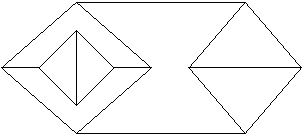
\includegraphics{PicJointSlides/SeqG2.pdf}}\par
\end{minipage}
\begin{minipage}[b]{30mm}
\centering
\resizebox{26mm}{!}{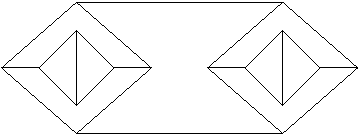
\includegraphics{PicJointSlides/SeqG3.pdf}}\par
\end{minipage}
\end{center}


\end{frame}

\begin{frame}\frametitle{$3$-connectedness of 
$(\{a,b\},6)$- and $(\{a,b\},4)$-spheres}
\vspace{-2mm}

\begin{itemize}
\item 
Any $(\{a,b\},6)$-sphere is $3$-connected, except  
$(\{2,3\},6)$- ones which  are duals of only $2$-connected
$(\{3,6\},3)$-spheres, with  six vertices 
of degree $2$
added on  edges.

%\item  Any $(\{1,3\},6)$- or $(\{3,4\},4)$-sphere  is $3$-connected.

\item
Any $(\{a,b\},4)$-sphere is $3$-connected, except
the  following series of $(\{2,4\},4)$-spheres.


\end{itemize}

\begin{center}
\begin{minipage}[b]{65mm}
\centering
\resizebox{55mm}{!}{\rotatebox{0}{\includegraphics{PicJointSlides/FamilyIinSec2.pdf}}}\par
\end{minipage}
\end{center}

%\begin{itemize}
%\item
REMARK. $\{2,4\}_v$($D_{2d}$,$D_{2h}$)  are
 {\em $k$-inflations} of above. $D_{4}$,$D_{4h}$
are  $GC_{k,l}(4$$\times$$ K_2)$. Remaining $D_2$: $2$ 
complex or $3$ natural  
parameters.
%\end{itemize}
\end{frame}



\begin{frame}\frametitle{Hamiltonicity of $(\{a,b\},k)$-spheres}
\begin{itemize}
\item \textcolor{blue}{Gr\H{u}nbaum-Zaks, 1974}:
all $(\{1,3\},6)$-
and $(\{2,4\},4)$-spheres are Hamiltonian, but $(\{2,6\},3)$-
with $v \equiv 0 \pmod 4$ are not
\item \textcolor{blue}{Goodey, 1977}:
 $(\{3,6\},3)$-
and $(\{4,6\},3)$- are Hamiltonian.
\item \textcolor{blue}{Conjecture}: an Hamiltonian circuit exists in
all other cases.
\end{itemize}
%\pause
To check hamiltonicity of  a $(\{a,b\},k)$-map on the 
projective plane $\mathbb{P}^2$, the 
following theorem
(\textcolor{blue}{Thomas-Yu, 1994}) could help: 

every $4$-connected graph 
on $\mathbb{P}^2$ 
has
a {\em contractible} (i.e. being a boundary of $2$-cell) Hamiltonian circuit.


\end{frame}
\section[]{Listing of $(\{a,b\},k)$-spheres with small $p_b$}

\frame{
\begin{center}
\begin{tabular*}{7cm}{c}
\\[-0.5cm]
{\Huge \textcolor{blue}{II'. }\textcolor{red}{ 
$(\{a,b\},k)$-spheres}}
\\[4mm]{\Huge \textcolor{red}{
with small $p_b$: listings} }
\end{tabular*}
\end{center}}


\begin{frame}\frametitle{$(\{a,b\},k)$-spheres with  
\textcolor{red}{$p_b\le 2$}$<a<b$}
\vspace{-3.5mm}

\begin{itemize}
\item 
Remind:
$(a,k)$=$(3,3),(4,3),(3,4),(5,3), (3,5)$ if $k,a\ge 3$.

\item 
The only $(\{a,b\},k)$-spheres with \textcolor{red}{$p_b\le 1$} are 
$5$  \textcolor{blue}{Platonic $(a^k)$}:

Tetrahedron, Cube ($Prism_4$), Octahedron ($APrism_3$), Dodecahedron (snub 
$Prism_5$), Icosahedron (snub $APrism_3$). 

\item  
There exists unique \textcolor{blue}{trivial}
$3$-connected $(\{a,b\},k)$-sphere with \textcolor{red}{$p_b$=$2$} 
for
$(\{4,b\},3)$-, $(\{3,b\},4)$-,  $(\{5,b\},3)$-,
$(\{3,b\},5)$-:

$D_{bh}$ \textcolor{blue}{$Prism_b$}  and $D_{bd}$  
\textcolor{blue}{$APrism_b$}, 
\textcolor{blue}{snub $Prism_b$}, \textcolor{blue}{snub $APrism_b$}:   

two
$b$-gons separated by $b$-ring
of $4$-gons, $2b$-ring
of $3$-gons, 

two $b$-rings of $5$-gons, two $3b$-rings of $3$-gons.
%Doubled $b$-gon $D_{bh}$ is such $(\{2,b\},4)$-sphere.


\item 
Also, for $t$$\ge$$2$, 
 $10$ 
\textcolor{blue}{non-trivial}  $(\{a,at\},k)$-spheres with 
\textcolor{red}{$p_{at}$=$2$}:
%See below all such $(\{a,2a\},3)$-spheres, each 
%of symmetry $D_{2h}$.
%$(a,k)$=$(3,3),(3,4),(4,3),(3,5),(5,3)$,
%there is unique only $2$-connected such sphere ($D_{2h}$) 
%iff $b\equiv 0\,(mod\,a)$.
%divides $b$.
%\pause

$5$ 
%$2$-edge-connected 
$(\{a,ta\},k)$-spheres are ($D_{th}$)
\textcolor{red}{necklaces} of polycycles $\{a^k\}$-$e$,

 $3$ are ($D_{th}$)  \textcolor{red}{necklaces} of $t$ $v$-split
$\{3^4\}$ and $e$-split
 $\{5^3\}$, $\{3^5\}$,                              

 $(\{3,3t\},5)$-spheres $C_{th}$, $D_t$
are \textcolor{red}{necklaces} of $t$ $v$-, $f$-split $\{3^5\}$.
\end{itemize}
\end{frame}

\begin{frame}\frametitle{$(\{a,ta\},k)$-spheres with
\textcolor{red}{$p_{ta}=2$}, $k$=$3,4,5$; case $t$=$2$}
\vspace{-3.5mm}
\begin{center}
\begin{minipage}[b]{16mm}
\centering
\epsfig{height=15mm, file=PicJointSlides/3reg_PB2/3reg_a3_b6_sec.pdf}\par
$D_{2h}$: $a$=$3$
\end{minipage}
\begin{minipage}[b]{16mm}
\centering
\epsfig{height=16mm, file=PicJointSlides/3reg_PB2/3reg_a4_b8_sec.pdf}\par
 $a$=$4$
\end{minipage}  
\begin{minipage}[b]{16mm}
\centering
\epsfig{height=16mm, 
file=PicJointSlides/3reg_PB2/3reg_a5_b10_b_sec.pdf}\par
$a$=$5$
\end{minipage}
\begin{minipage}[b]{16mm}
\centering
\epsfig{height=16mm, 
file=PicJointSlides/3reg_PB2/3reg_a5_b10_a_sec.pdf}\par
$a$=$5$
\end{minipage}
\end{center}


\begin{center}
\begin{minipage}[b]{17mm}
\centering
\epsfig{height=16mm, file=PicJointSlides/4reg_PB2/4reg_a3_b6_aSec.pdf}\par
$a$=$3$ $D_{2h}$
\end{minipage}
\begin{minipage}[b]{17mm}
\centering
\epsfig{height=17mm, file=PicJointSlides/4reg_PB2/4reg_a3_b6_bSec.pdf}\par
%$k$=$4$, 
$a$=$3$ $D_{2h}$
\end{minipage}  
\end{center}
\vspace{-2mm}
%\end{frame}

\begin{center}
\begin{minipage}[b]{17mm}
\centering
\epsfig{height=15mm, file=PicJointSlides/5reg_PB2/PL3b_sec.pdf}\par
$a$=$3$ $D_{2h}$
\end{minipage}
\begin{minipage}[b]{17mm}
\centering
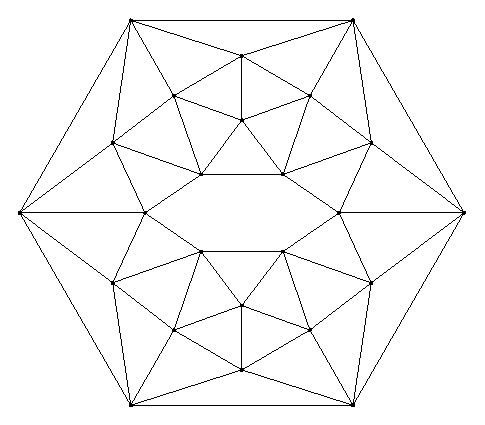
\epsfig{height=16mm, file=PicJointSlides/5reg_PB2/PL_D2h_b2_sec.pdf}\par
%$k$=$5$ 
$a$=$3$ $D_{2h}$
\end{minipage}  
\begin{minipage}[b]{17mm}
\centering
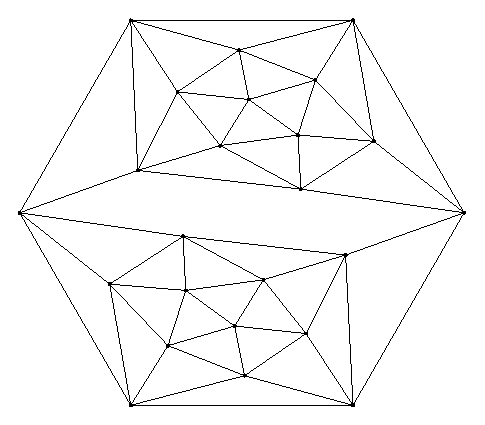
\epsfig{height=16mm, file=PicJointSlides/5reg_PB2/PL10_sec.pdf}\par
%$k$=$5$ 
$a$=$3$ $C_{2h}$
\end{minipage}
\begin{minipage}[b]{17mm}
\centering
\epsfig{height=16mm, file=PicJointSlides/5reg_PB2/PL_dcdSec.pdf}\par
$a$=$3$ $D_{2}$
\end{minipage}
\end{center}
\end{frame}

\begin{frame}\frametitle{Proof method: elementary $(a,k)$-polycycles}
\vspace{-3.5mm}
\begin{itemize}
\item A \textcolor{red}{$(a,k)$-polycycle} is a
$2$-connected plane graph with faces partitioned
in  $a$-gonal
%two families: $F_1$  (
\textcolor{blue}{proper  faces} and 
%$F_2$ 
%(pairwisely disjoint 
\textcolor{blue}{holes}, exterior face among them, 
so that
vertex degrees are  in $\{2,\dots ,k\}$ and  can be  $<k$
only for a  vertex lying on the
boundary of a hole.
\item Any $(a,k)$-polycycle \textcolor{red}{decomposes uniquely} along 
its \textcolor{blue}{bridges} (non-boundary  going   
hole-to-hole, possibly, same, edges)

into  \textcolor{red}{elementary} ones. Cf. integer factorisation into 
primes.  
\item We listed them for $\frac{1}{a}$ +$\frac{1}{k}-\frac{1}{2}$$\ge$$0$. Othervise, 
continuum...  
\end{itemize}

\begin{center}
\begin{minipage}[b]{20mm}
\centering
\epsfig{height=19mm, file=PicJointSlides/3reg_PB3/PL5_15_5_Cs_exmpB.pdf}\par
%Decomposition
%osition 
%of a $(\{5,15\},3)$-sphere into elementary
%polycycles edge-split $\{5^3\}$, $Pen_1$, $\{5^3\} - e$ and $C_2$
\end{minipage}
%\begin{minipage}[b]{17mm}
%\centering
%\epsfig{height=16mm, file=}\par
%$\{5^3\}-e$
%\end{minipage}
\end{center} 
This $(\{5,15\},3)$-sphere with $p_{15}$=$3$ 
is a $3$-holes $(\{5\},3)$-polycycle 

It decomposes into five
$1$-hole elementary $(\{5\},k)$-polycycles.

\end{frame} 

%\begin{minipage}[b]{17mm}
%\centering
%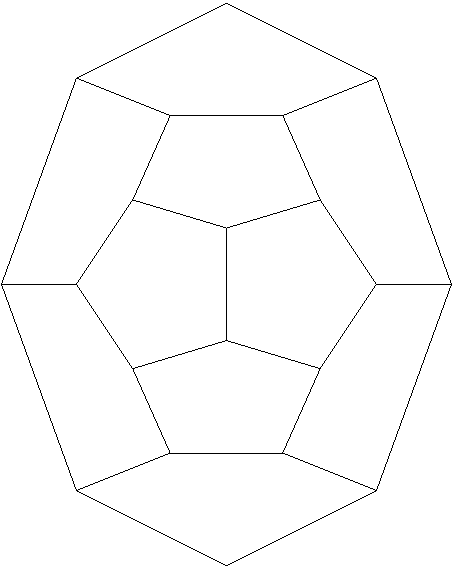
\epsfig{height=17mm, 
%file=PicJointSlides/ElemPresPic/PolycycleA2_NC.pdf}\par $\{5^3\}-e$
%\end{minipage}
%\end{center}\vspace{-2mm}

%\begin{center}\begin{minipage}[b]{17mm}\centering
%\epsfig{height=16mm, file=PicJointSlides/ElemPresPic/34poly_RT.pdf}\par
%$v$-split $\{3^4\}$\end{minipage} \begin{minipage}[b]{17mm}\centering
%.\end{minipage}   \begin{minipage}[b]{17mm}\centering
%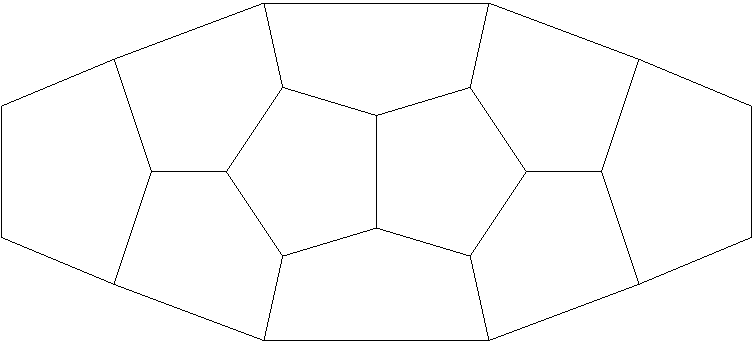
\epsfig{height=16mm,file=PicJointSlides/ElemPresPic/Fundamental22polycycle3_NC.pdf}\par
%$e$-split $\{5^3\}$\end{minipage}\end{center}


\begin{frame}\frametitle{$(\{a,b\},3)$-spheres with
$\textcolor{red}{p_b=3}$}
\begin{itemize}

\item   $(\{a,b\},k)$-sphere with \textcolor{red}{$p_b=3$} exists
if and only if
$b\equiv 2,a,2a-2\,(mod\,2a)$ and  $b\equiv 4,6\,(mod\,10)$
if $a$=$5$.
\item  Such sphere are unique if $b$ is not
$\equiv a\,(mod\,2a)$ and then their symmetry is $D_{3h}$, except when
$(a,k)=(3,5)$ when the symmetry is $D_3$.
 

\item There are $7$ such spheres with $t$=$\lfloor{\frac{b}{6}}\rfloor$=$0$
and 

$3$+$4$+$5$+$17$ of them for any $t\ge 1$.
\end{itemize}
\end{frame}     




\begin{frame}\frametitle{\textcolor{red}{$(\{3,b\},3)$}- and 
\textcolor{red}{$(\{4,b\},3)$}-spheres with \textcolor{red}{$p_b=3$}}
\vspace{-3mm}

\begin{itemize}
\item
Such $(\{3,b\},3)$-sphere  exists \textcolor{red}{iff} $b\equiv 2,3,4\,(mod\,6)$:

unique  ($D_{3h}$, $C_{3v}$, $D_{3h}$), respectively,  and
comes  by putting $t$=$\lfloor{\frac{b}{6}}\rfloor$  $\{3^3\}$-$e$'s on $3$ edges of 
$3K_2$, $Prism_3$,  Tetrahedron $\{3^3\}$.
\end{itemize}


\begin{center}
\begin{minipage}[b]{19mm}
\centering
\epsfig{height=17mm, file=PicJointSlides/Prism3sec.pdf}\par
%cat_PL4_6_1_2d-1.pdf}\par
$b$=$4$, $D_{3h}$
\end{minipage}
\begin{minipage}[b]{19mm}
\centering
\epsfig{height=17mm, file=PicJointSlides/3reg_PB3/PL3_8_1_D3hsec.pdf}\par 
%cat_PL4_10_1-2d-1.pdf}\par
$2$+$6$, $D_{3h}$
\end{minipage}  
\begin{minipage}[b]{19mm}
\centering
\epsfig{height=17mm, file=PicJointSlides/3reg_PB3/PL3_9_1_C3vSec.pdf}\par 
%cat_PL4_12_1-2d-1.pdf}\par
$3$+$6$, $C_{3v}$
\end{minipage}
\begin{minipage}[b]{19mm}
\centering
\epsfig{height=17mm, file=PicJointSlides/3reg_PB3/PL3_10_1_D3h_sec.pdf}\par 
%cat_PL4_12_2-2d-1.pdf}\par
$4$+$6$, $D_{3h}$
\end{minipage}
\end{center}
\vspace{-4mm}


\begin{center}
\begin{minipage}[b]{19mm}
\centering
\epsfig{height=17mm, 
file=PicJointSlides/3reg_PB3/PL4_6_1_D3h_sec.pdf}\par
%cat_PL4_6_1_2d-1.pdf}\par
$b$=$6$, $D_{3h}$
\end{minipage}
\begin{minipage}[b]{19mm}
\centering
\epsfig{height=17mm, 
file=PicJointSlides/3reg_PB3/PL4_10_1_D3h_sec.pdf}\par
%cat_PL4_10_1-2d-1.pdf}\par
$2$+$8$, $D_{3h}$
\end{minipage}  
\begin{minipage}[b]{19mm}
\centering
\epsfig{height=17mm, file=PicJointSlides/3reg_PB3/PL4_12_1_C3v_sec.pdf}\par
%cat_PL4_12_1-2d-1.pdf}\par
$4$+$8$, $C_{3v}$
\end{minipage}
\begin{minipage}[b]{19mm}
\centering
\epsfig{height=17mm, file=PicJointSlides/3reg_PB3/PL4_12_2_C2v_sec.pdf}\par
%cat_PL4_12_2-2d-1.pdf}\par
$4$+$8$, $C_{2v}$
\end{minipage}
\end{center}
\begin{itemize}
\item
Such $(\{4,b\},3)$-sphere  exists \textcolor{red}{iff} $b\equiv 2,4,6\,(mod\,8)$:
$2$ ($C_{3v}$, $C_{2v}$) if $b\equiv 4\,(mod\,8)$ and unique ($D_{3h}$),
 otherwise.
\end{itemize}

\end{frame}



\begin{frame}\frametitle{$(\{\textcolor{red}{(\{3,b\},4)}$-spheres with
$\textcolor{red}{p_b=3}$}
\vspace{-2mm}
\begin{itemize}
\item 
  Such ${(\{3,b\},4)}$-sphere  exists \textcolor{red}{iff} $b\equiv 
2,3,4\,(mod\,6)$:

$3$ ($C_{3v},C_s,C_s$) if $b\equiv 3\,(mod\,6)$ and unique ($D_{3h}$), otherwise.

\item For $b$=$2$+$6t$, $4$+$6t$ and  $C_{3v}$-case of $3$+$6t$,  
it is $3K_2$, $9$-vertex $(\{3,b\},4)$-sphere,  Octahedron $\{3^4\}$
    with $3$ edges replaced by
$t$ $v$-split
 $\{3^4\}$'s.
It is
\textcolor{blue}{$3$-connected} iff $b$=$2,4$.
\end{itemize}
\vspace{-3mm}   
\begin{center}
\begin{minipage}[b]{19mm}
\centering    
\epsfig{height=17mm, file=PicJointSlides/Example4reg.pdf}\par
%PL_4reg_3_4_9_1_D3h_sec.pdf}\par  
$D_{3h}$, $b$=$2$
\end{minipage} 
\begin{minipage}[b]{19mm}
\centering
\epsfig{height=17mm, file=PicJointSlides/4reg_PB3/PL_4reg_3_4_9_1_D3h_sec.pdf}\par
%PL_4reg_3_8_21_1_D3h_sec.pdf}\par
$b$=$4$
\end{minipage}
\begin{minipage}[b]{19mm}
\centering
\epsfig{height=17mm, file=PicJointSlides/4reg_PB3/PL_4reg_3_8_21_1_D3h_sec.pdf}\par
%PL_4reg_3_9_24_3_Cs_sec.pdf}\par
$b$=$2$+$6$
%, $D_{3}$
\end{minipage}
\begin{minipage}[b]{19mm}
\centering 
\epsfig{height=17mm, file=PicJointSlides/4reg_PB3/PL_4reg_3_10_27_1_D3h_sec.pdf}\par
%PL_4reg_3_10_27_1_D3h_sec.pdf}\par
$b$=$4$+$6$
\end{minipage}
\end{center} 

\begin{center}
\begin{minipage}[b]{19mm}
\centering
\epsfig{height=17mm, file=PicJointSlides/4reg_PB3/PL_4reg_3_9_24_1_C3v_sec.pdf}\par
%PL_4reg_3_9_24_1_C3v_sec.pdf}\par
$3$+$6$, $C_{3v}$
\end{minipage}
\begin{minipage}[b]{19mm}
\centering
\epsfig{height=17mm, file=PicJointSlides/4reg_PB3/PL_4reg_3_9_24_2_Cs_sec.pdf}\par
%PL_4reg_3_9_24_2_Cs_sec.pdf}\par
$3$+$6$, $C_s$
\end{minipage}
\begin{minipage}[b]{19mm}
\centering   
\epsfig{height=17mm, file=PicJointSlides/4reg_PB3/PL_4reg_3_9_24_3_Cs_sec.pdf}\par
%PL_4reg_3_9_24_3_Cs_sec.pdf}\par
$3$+$6$, $C_{s}$
\end{minipage}
\end{center}

\end{frame} 



\begin{frame}\frametitle{$\textcolor{red}{(\{5,b\},3)}$- 
and $\textcolor{red}{(\{3,b\},5)}$-spheres with
$\textcolor{red}{p_b=3}$}
\vspace{-3mm}
  
Such ${(\{5,b\},3)}$-sphere  exists
\textcolor{red}{iff}
$b\equiv 2,4,5,6,8\,(mod\,10)$:  

$5$ ($2$ $C_{3v}$ and $2$ $C_s$) if $b\equiv 
5\,(mod\,10)$
and unique ($D_{3h}$), otherwise.



\begin{center}
\begin{minipage}[b]{19mm}
\centering
\epsfig{height=17mm, file=PicJointSlides/Spec45sec.pdf}\par
%cat_PL5_6_1-2d-1
%$b$=$6$
$D_{3h}$: $b$=$4$ 
\end{minipage}
\begin{minipage}[b]{19mm}
\centering
\epsfig{height=17mm, file=PicJointSlides/3reg_PB3/PL5_6_1_D3h_sec.pdf}\par
%cat_PL5_8_1-2d-1
%$8$ 
$b$=$6$ 
\end{minipage}
\begin{minipage}[b]{19mm}
\centering   
\epsfig{height=17mm, file=PicJointSlides/3reg_PB3/PL5_8_1_D3h_sec.pdf}\par
%cat_PL5_12_1_2d-1
%$2$+$10$
$b$=$8$ 
\end{minipage}
\begin{minipage}[b]{19mm}
\centering
\epsfig{height=17mm, 
file=PicJointSlides/3reg_PB3/PL5_12_1_D3h_sec.pdf}\par
%cat_PL5_14_1_2d-1
%$b=2$+$10$
$b$=$2$+$10$ 
\end{minipage}
\end{center}

\begin{center}
\begin{minipage}[b]{19mm}
\centering
\epsfig{height=18mm, file=PicJointSlides/First_Pb2.pdf}\par
%PL5_15_1_C3v_sec
%$5$+$10$, $C_{3v}$
$D_3$: $b$=$2$
\end{minipage}
\begin{minipage}[b]{19mm}
\centering
\epsfig{height=17mm, file=PicJointSlides/PLminD3_18sec.pdf}\par
%PL5_15_2_Cs_sec
%$15$, $C_{s}$
$b$=$4$
\end{minipage}
\begin{minipage}[b]{19mm}
\centering
\epsfig{height=17mm, file=PicJointSlides/5reg_PB3/PL13_sec.pdf}\par
%PL5_15_4_C3v_sec
%$15$, $C_{3v}$
$b$=$2$+$6$
\end{minipage}
\begin{minipage}[b]{19mm}
\centering
\epsfig{height=17mm, file=PicJointSlides/5reg_PB3/PL14_sec.pdf}\par
%PL5_15_5_Cs_sec
%$15$, $C_{s}$
$b$=$4$+$6$
\end{minipage}
\end{center}
%\end{itemize}

Such ${(\{3,b\},5)}$-sphere  exists
if
$b\equiv 2,3,4\,(mod\,6)$:

$15$  if $b\equiv 3\,(mod\,6)$
and one ($D_{3}$), 
%for each of $b\equiv 2,4\,(mod\,6)$, 
otherwise.

\end{frame}


\section[]{$8$ standard families: four  smallest members}

\frame{
\begin{center}
\begin{tabular*}{7cm}{c}
\\[-0.5cm]
{\Huge \textcolor{blue}{III. }\textcolor{red}{
$8$ standard families:}}
%$8$ families:}}
\\[4mm]{\Huge \textcolor{red}{
$4$ smallest members}
}
\end{tabular*}
\end{center}
}




\begin{frame}\frametitle{First four $(\{2,4\},4)$- and  $(\{3,4\},4)$-spheres}
\vspace{-4mm}
\begin{center}
\begin{minipage}[b]{24mm}
\centering
\resizebox{20mm}{!}{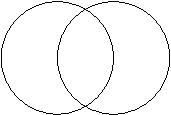
\includegraphics{PicJointSlides/4-hedrite2_1.pdf}}\par
$D_{4h}$ \textcolor{blue}{$2^2_1$} $(2^2)$
\end{minipage}
\begin{minipage}[b]{21mm}
\centering
\resizebox{18mm}{!}{\includegraphics{PicJointSlides/4-hedrite4_1.pdf}}\par
$D_{4h}$ \textcolor{blue}{$4^2_1$}  $(4^2)$
\end{minipage}
\begin{minipage}[b]{29mm}
\centering
\resizebox{24mm}{!}{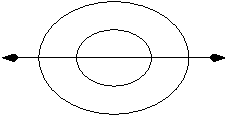
\includegraphics{PicJointSlides/4-hedrite4-2.pdf}}\par
$D_{2h}$ 
\textcolor{blue}{$2$$\times$$ 2^2_1$} 
 $(2^2,4)$ 
\end{minipage}
\begin{minipage}[b]{24mm}
\centering
\resizebox{20mm}{!}{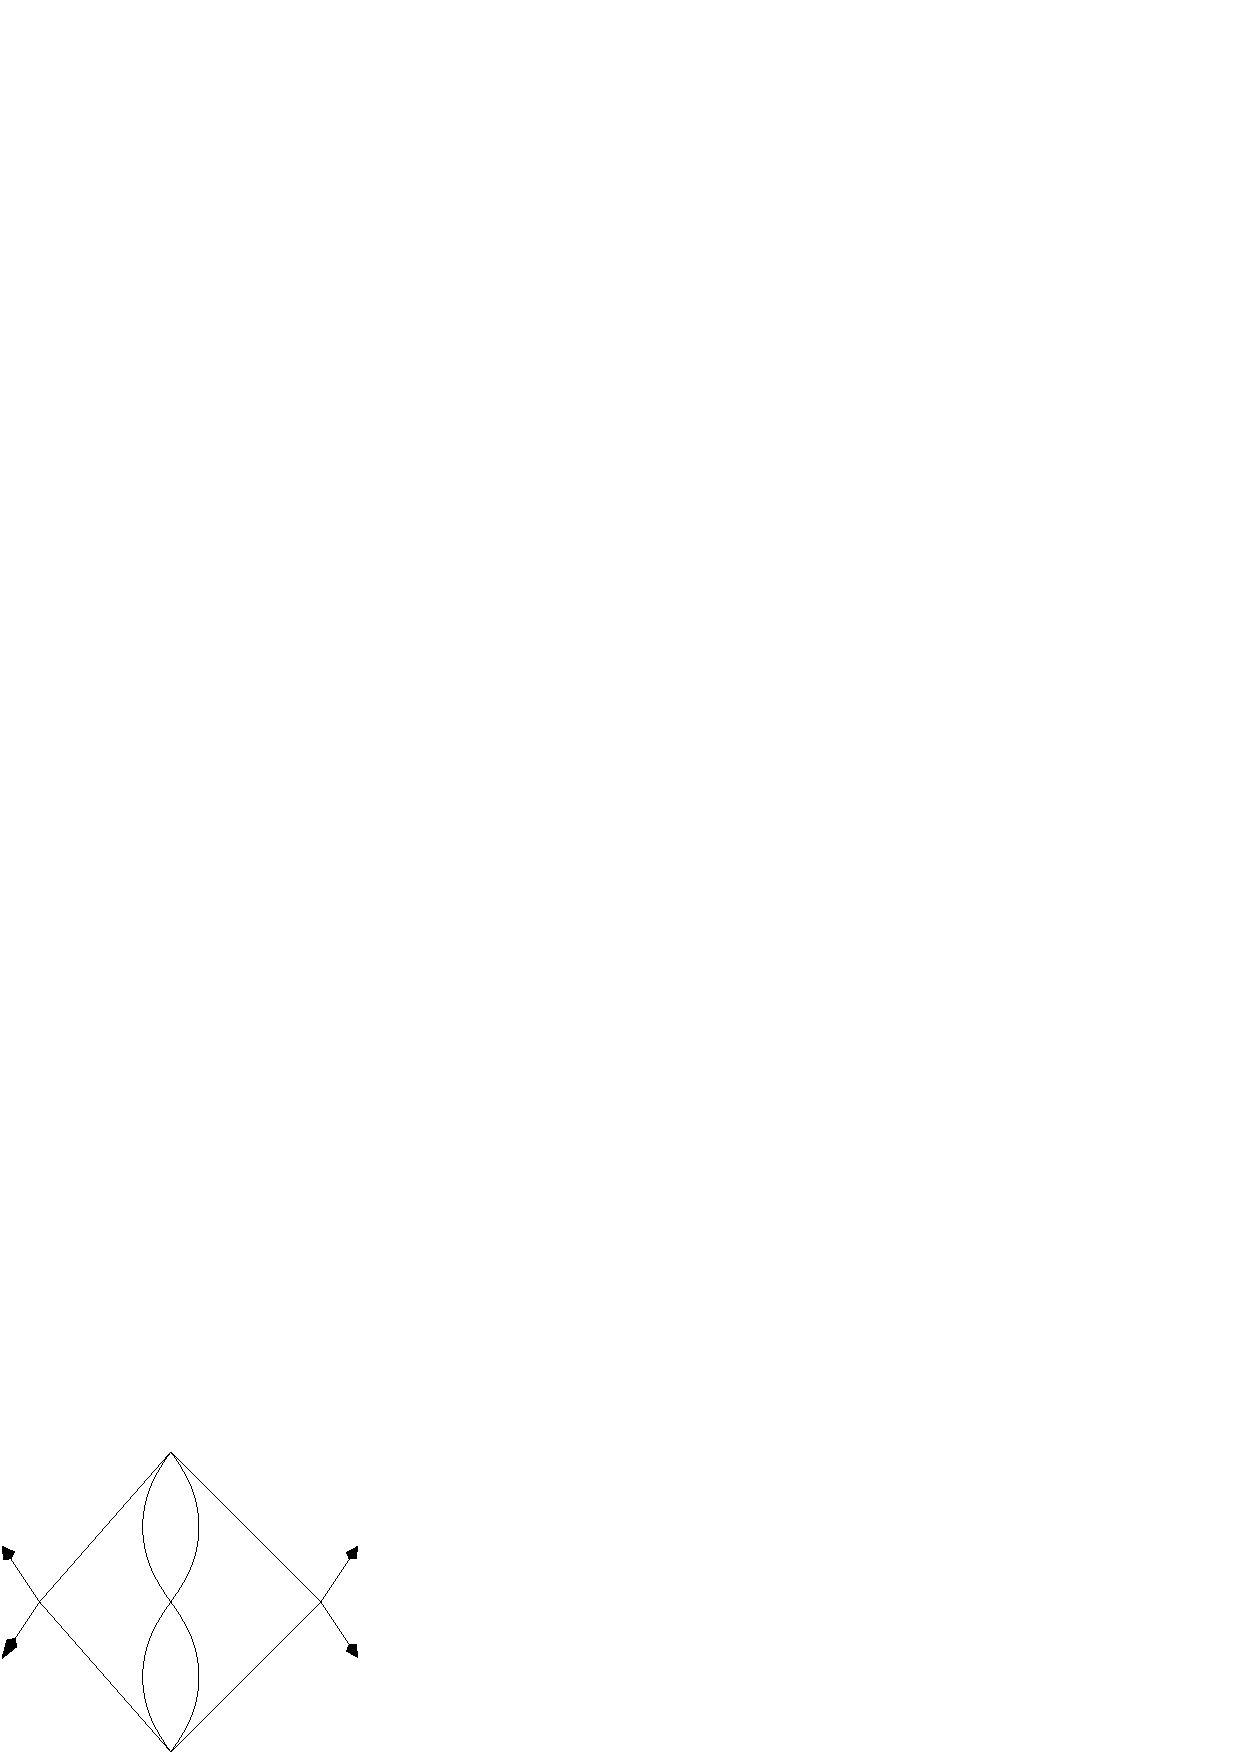
\includegraphics{PicJointSlides/4-hedrite6_1sec.pdf}}\par
%\textcolor{blue}{$6^2_2$}  
$D_{2d}$ \textcolor{blue}{$6^2_2$}  $(6^2)$
\end{minipage}
\end{center}

\begin{center}
\begin{minipage}[b]{24mm}
\centering     
\resizebox{20mm}{!}{\includegraphics{PicJointSlides/8-hedrite6-1.pdf}}\par
$O_h$ \textcolor{blue}{$6^3_2$} $(4^3)$\\
Borr. rings
\end{minipage}
\begin{minipage}[b]{24mm}
\centering
\resizebox{20mm}{!}{\includegraphics{PicJointSlides/8-hedrite8-1.pdf}}\par
$D_{4d}$ \textcolor{blue}{$8_{18}$} $(16)$
\end{minipage}
\begin{minipage}[b]{23mm}
\centering
\resizebox{19mm}{!}{\includegraphics{PicJointSlides/8-hedrite9_1.pdf}}\par
$D_{3h}$ \textcolor{blue}{$9_{40}$} $(18)$\\
(Herschel)$^{*}$
\end{minipage}
\begin{minipage}[b]{23mm}
\centering
\resizebox{19mm}{!}{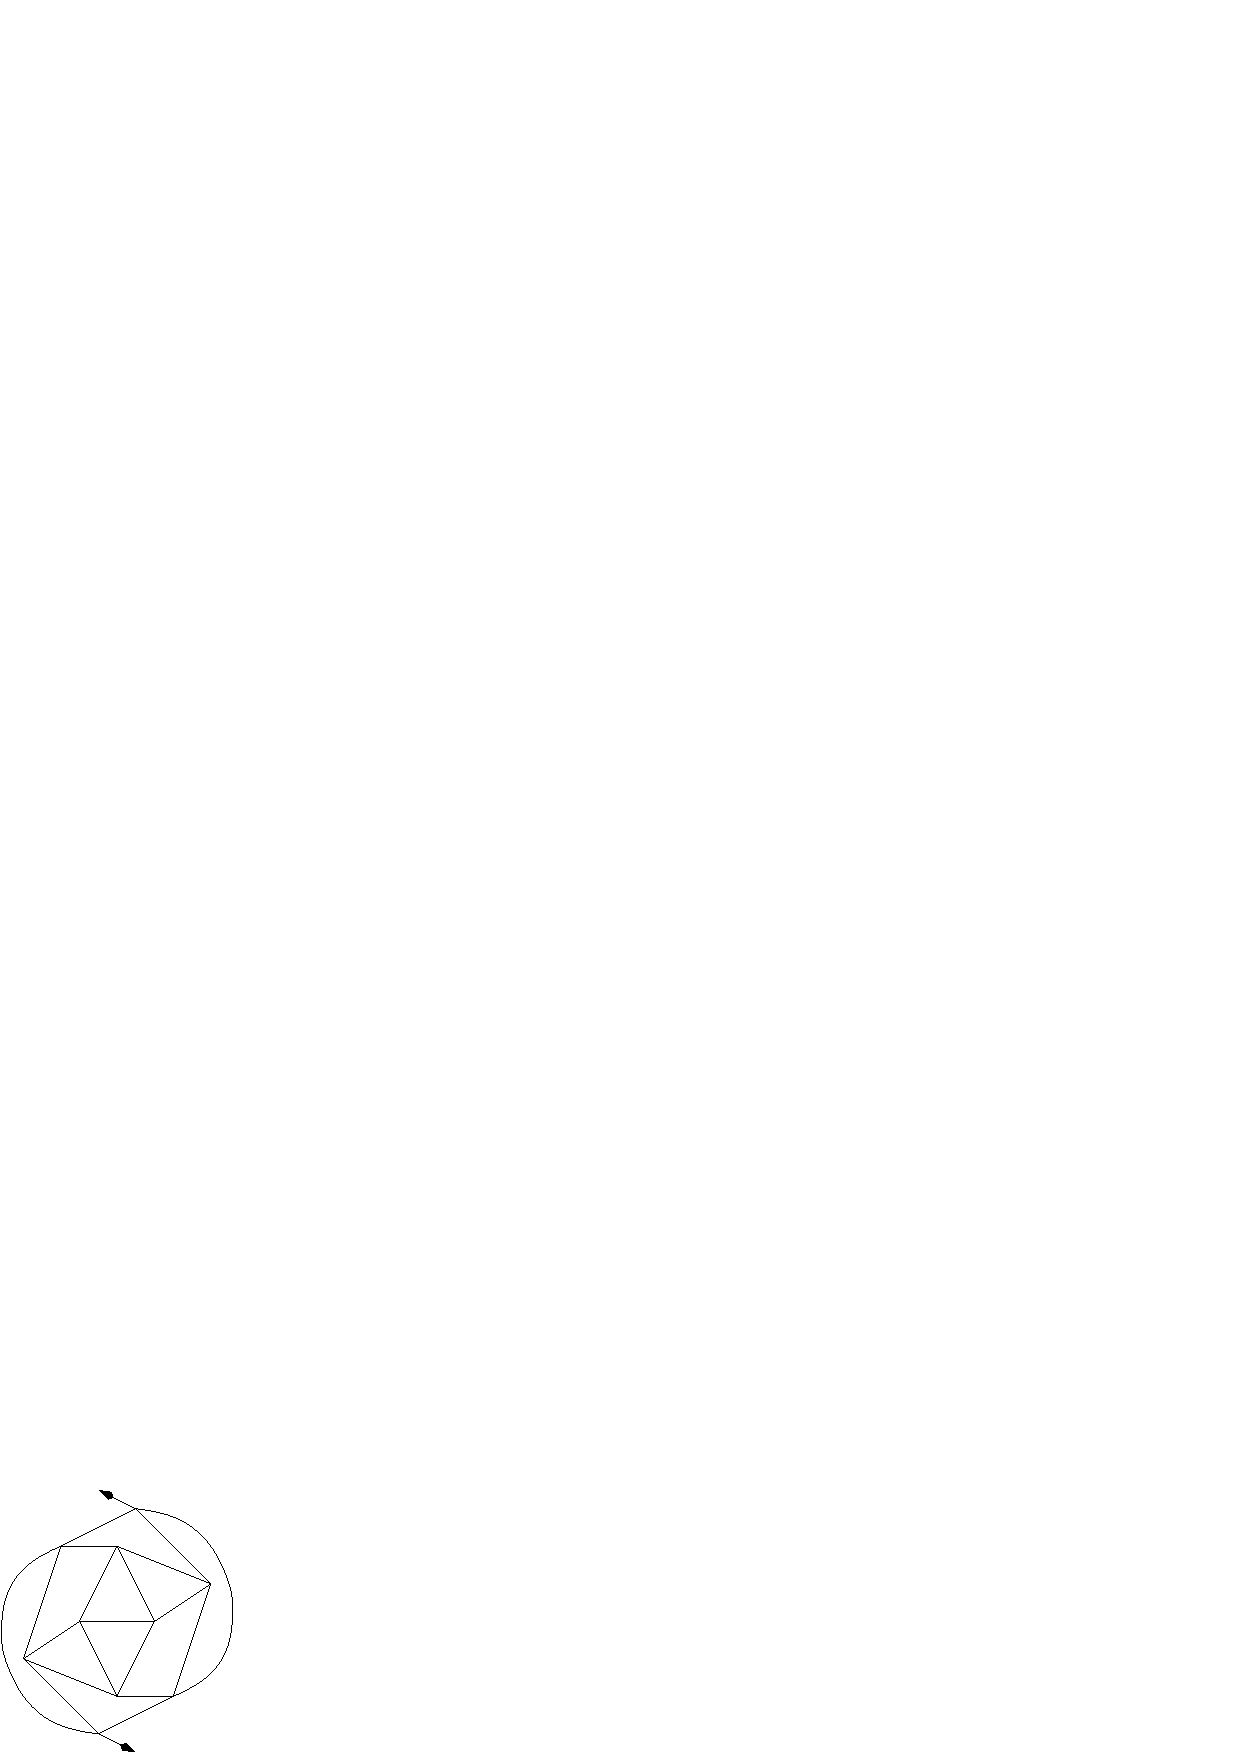
\includegraphics{PicJointSlides/8-hedrite10_1sec.pdf}}\par
%\resizebox{19mm}{!}{\rotatebox{90}{\includegraphics{PicJointSlides/8-hedrite10_1sec.pdf}}}\par
$D_{2}$ 
\textcolor{blue}{$10^2_{56}$} 
 $(6;14)$
\end{minipage}
\end{center}
Above links/knots  are given in \textcolor{blue}{Rolfsen, 1976 and 1990} 
 notation.

Herschel graph: the smallest non-Hamiltonian polyhedral graph.
\end{frame}

\begin{frame}\frametitle{First four $(\{2,3\},6)$- and
$(\{1, 3\},6)$-spheres}
\vspace{-2.5mm}

\begin{center}
\begin{minipage}[b]{26mm}
\centering
\resizebox{22mm}{!}{\includegraphics{PicJointSlides/Bundle6.pdf}}\par
$D_{6h}$ ($2^3$)
\end{minipage}  
\begin{minipage}[b]{23mm}
\centering
\resizebox{19mm}{!}{\includegraphics{PicJointSlides/Example23_6val_1.pdf}}\par
$D_{3h}$ ($3;6$)
\end{minipage}
\begin{minipage}[b]{24mm}
\centering
\resizebox{20mm}{!}{\includegraphics{PicJointSlides/23graph_3R2_2.pdf}}\par
$D_{2d}$ ($2^2;8$)
\end{minipage}
\begin{minipage}[b]{23mm}
\centering
\resizebox{19mm}{!}{\includegraphics{PicJointSlides/Example23_6val_2.pdf}}\par
$T_{d}$ ($3^4$)
\end{minipage}
\end{center}



\begin{center}
\begin{minipage}[b]{25mm}
\centering
\resizebox{20mm}{!}{\includegraphics{PicJointSlides/Class_C3_C3vB.pdf}}\par
$C_{3v}$  ($3$)
\end{minipage} 
\begin{minipage}[b]{25mm}
\centering
\resizebox{17mm}{!}{\includegraphics{PicJointSlides/Singular13_3vert.pdf}}\par
$C_{3h}$ ($3;6$)
\end{minipage}
\begin{minipage}[b]{25mm}
\centering
\resizebox{18mm}{!}{\includegraphics{PicJointSlides/Class_C3_C3v.pdf}}\par
%\resizebox{20mm}{!}{\rotatebox{90}{\includegraphics{PicJointSlides/PLdual9_sec.pdf}}}\par
$C_{3v}$ ($6^2$)
\end{minipage}
\begin{minipage}[b]{25mm}
\centering
%\resizebox{18mm}{!}{\includegraphics{PicJointSlides/Class_C3_C3_sec.pdf}}\par
\resizebox{20mm}{!}{\rotatebox{90}{\includegraphics{PicJointSlides/Class_C3_C3_sec.pdf}}}\par
$C_{3}$  ($21$)
\end{minipage} 
%\begin{minipage}[b]{25mm}
%\centering
%%\resizebox{18mm}{!}{\includegraphics{PicJointSlides/PLdual9_sec.pdf}}\par
%\resizebox{20mm}{!}{\rotatebox{90}{\includegraphics{PicJointSlides/PLdual9_sec.pdf}}}\par
%$C_{3v}$ ($9^3$)
%\end{minipage}
\end{center}


\textcolor{blue}{Gr\H{u}nbaum-Zaks, 1974}: $\{1,3\}_v$ exists iff
$v=k^2+kl+l^2$ for integers $0\le l\le k$.
We show that the
number of
  $\{1,3\}_v$'s is the number  of such representations of $v$, i.e.
found
 $GC_{k,l}(\{1,3\}_1)$.

\end{frame}



\begin{frame}\frametitle{First four $(\{2,6\},3)$- and
$(\{3,6\},3)$-spheres}
\vspace{-1.5mm}
 Number  of $(\{2,6\}_v$'s is nr. of representations $v$=$2(k^2+kl+l^2)$,  
$0\le l\le k$ ($GC_{k,l}(\{2,6\}_2)$). It become $2$ for 
$v$=$7^2$=$5^2$+$15$+$3^2$.

\begin{center}
\begin{minipage}[b]{25mm}
\centering
\resizebox{21mm}{!}{\includegraphics{PicJointSlides/First2nD3h.pdf}}\par
$D_{3h}$ ($6$)
\end{minipage}
\begin{minipage}[b]{23mm}
\centering
\resizebox{19mm}{!}{\includegraphics{PicJointSlides/GC11Bundle.pdf}}\par
$D_{3h}$ ($6^3$)
\end{minipage}
\begin{minipage}[b]{18mm}
\centering
\resizebox{16mm}{!}{\includegraphics{PicJointSlides/GC20Bundle.pdf}}\par
$D_{3h}$  ($12^2$)
\end{minipage}
\begin{minipage}[b]{28mm}
\centering
\resizebox{22mm}{!}{\includegraphics{PicJointSlides/FirstClass2nD3.pdf}}\par
%\resizebox{20mm}{!}{\rotatebox{90}{\includegraphics{PicJointSlides/FirstClass2nD3.pdf}}}\par 
$D_{3}$ ($42$)
\end{minipage}
\end{center}



\begin{center}
\begin{minipage}[b]{20mm}
\centering
%\resizebox{18mm}{!}{\includegraphics{PicJointSlides/TetrahedronH.pdf}}\par
\resizebox{20mm}{!}{\rotatebox{90}{\includegraphics{PicJointSlides/TetrahedronH.pdf}}}\par
$T_d$ ($4^3$)
\end{minipage}
\begin{minipage}[b]{29mm}
\centering
\resizebox{24mm}{!}{\includegraphics{PicJointSlides/SeqG1.pdf}}\par
$D_{2h}$ ($8^2,4^2$)
\end{minipage}
\begin{minipage}[b]{20mm}
\centering
\resizebox{20mm}{!}{\includegraphics{PicJointSlides/TruncatedTetrahedronNaked.pdf}}\par
$T_d$ ($12^3$)
\end{minipage}
\begin{minipage}[b]{24mm}
\centering    
\resizebox{20mm}{!}{\includegraphics{PicJointSlides/ebe1.pdf}}\par
 $T_d$ $(8^6)$
\end{minipage}
\end{center}  


\end{frame}

\begin{frame}\frametitle{First four $(\{4,6\},3)$- and
$(\{5,6\},3)$-spheres}


\begin{center}
\begin{minipage}[b]{24mm}
\centering
%\resizebox{20mm}{!}{\includegraphics{PicJointSlides/Prism4.pdf}}\par
\resizebox{20mm}{!}{\rotatebox{90}{\includegraphics{PicJointSlides/Prism4.pdf}}}\par
$O_h$ ($6^4$)
\end{minipage}
\begin{minipage}[b]{25mm}
\centering
\resizebox{21mm}{!}{\includegraphics{PicJointSlides/Prism6.pdf}}\par
$D_{6h}$ ($18^2$)
\end{minipage}
\begin{minipage}[b]{24mm}
\centering
%\resizebox{20mm}{!}{\includegraphics{PicJointSlides/First4nD3hthi.pdf}}\par
\resizebox{20mm}{!}{\rotatebox{90}{\includegraphics{PicJointSlides/First4nD3hthi.pdf}}}\par
$D_{3h}$ ($6^2;30$)
\end{minipage}
\begin{minipage}[b]{23mm}
\centering
\resizebox{19mm}{!}{\includegraphics{PicJointSlides/First4nD2dthi.pdf}}\par
$D_{2d}$ ($24^2$)
\end{minipage}
\end{center}  




\begin{center}
\begin{minipage}[b]{24mm}
\centering
\resizebox{20mm}{!}{\rotatebox{90}{\includegraphics{PicJointSlides/F1.pdf}}}\par
%\resizebox{20mm}{!}{\includegraphics[bb=1 1 440 381,
%clip]{PicJointSlides/Dodecahedron.pdf}}\par
 $I_h$ ($10^6$)
\end{minipage}
\begin{minipage}[b]{24mm}
\centering
\resizebox{20mm}{!}{\includegraphics{PicJointSlides/F2sec-crop.pdf}}\par
%\resizebox{20mm}{!}{\includegraphics[bb=1 1 440 381,clip]{PicJointSlides/F2sec.pdf}}\par
 $D_{6d}$ ($12;60$) 
%($12;60_{12,12}$)
\end{minipage}
\begin{minipage}[b]{24mm}
\centering
\resizebox{20mm}{!}{\includegraphics{PicJointSlides/Picture2-crop.pdf}}\par
%\resizebox{20mm}{!}{\includegraphics[bb=1 1 457 464,clip]{PicJointSlides/Picture2.pdf}}\par
 $D_{3h}$ ($12^3;42$) 
%($12^3;42_{0,9}$)
\end{minipage}
\begin{minipage}[b]{24mm}
\centering
\resizebox{20mm}{!}{\includegraphics{PicJointSlides/F4sec-crop.pdf}}\par
%\resizebox{20mm}{!}{\includegraphics[bb=1 1 439 380,clip]{PicJointSlides/F4sec.pdf}}\par
 $T_{d}$ ($12^7$)
\end{minipage}
\end{center}  



\end{frame}

\section[]{Symmetry groups of $(\{a,b\},k)$-spheres}

\frame{
\begin{center}
\begin{tabular*}{7cm}{c}
\\[-0.5cm]
{\Huge \textcolor{blue}{IV. }\textcolor{red}{Symmetry groups  of}}
\\[4mm]{\Huge \textcolor{red}{$(\{a,b\},k)$-spheres}
}
\end{tabular*}
\end{center}
}



\begin{frame}\frametitle{Finite isometry groups}
\vspace{-1mm}


All finite groups of isometries of $3$-space $\mathbb{E}^3$ are 
classified. 

In Schoenflies notations, they are:
\begin{itemize}
\item $C_1$ is the \textcolor{blue}{trivial} group
\item $C_s$ is the group generated by a \textcolor{blue}{plane reflexion}
\item $C_i=\{I_3, -I_3\}$ is the \textcolor{blue}{inversion} group
\item $C_m$ is the group generated by a \textcolor{blue}{rotation} of 
order 
$m$ of axis $\Delta$
\item $C_{mv}$ ($\simeq$ dihedral group) is the group generated by $C_m$ 
and $m$ \textcolor{blue}{reflexion containing} $\Delta$
\item $C_{mh}=C_m\times C_s$ is the group generated by $C_m$ and the 
\textcolor{blue}{symmetry by the plane orthogonal} to $\Delta$
\item $S_{2m}$ is the group of order $2m$ generated by an 
\textcolor{blue}{antirotation}, i.e. commuting composition of a rotation
and a plane symmetry
\end{itemize}
\end{frame}





\begin{frame}\frametitle{Finite isometry groups $D_m$, $D_{mh}$, $D_{md}$}

\begin{itemize}
\item $D_m$ ($\simeq$ dihedral group) is the group generated of $C_m$ and 
$m$ \textcolor{blue}{rotations of order $2$
with axis orthogonal} to $\Delta$
\item $D_{mh}$ is the group generated by $D_m$ and a 
\textcolor{blue}{plane symmetry orthogonal} to
$\Delta$
\item $D_{md}$ is the group generated by $D_m$ and $m$ 
\textcolor{blue}{symmetry planes containing}
$\Delta$ and which \textcolor{blue}{does not contain} axis of order $2$
\end{itemize}
%\pause

\begin{center}
\begin{minipage}{3.9cm}
\centering
\resizebox{3.8cm}{!}{\includegraphics{PicJointSlides/D2h.pdf}}\par
$D_{2h}$
\end{minipage}
\begin{minipage}{3cm}
\centering
\resizebox{2.7cm}{!}{\includegraphics{PicJointSlides/D2d.pdf}}\par
$D_{2d}$
\end{minipage}
\end{center}    


\end{frame}





\begin{frame}\frametitle{Remaining $7$ finite isometry groups}
\vspace{-1mm}
\begin{itemize} 
\item $I_h=H_3$ is the group of
\textcolor{blue}{isometries} of \textcolor{blue}{Dodecahedron};
$I_h\simeq Alt_5\times C_2$ 
\item $I\simeq Alt_5$ is the group of \textcolor{blue}{rotations} of Dodecahedron
\item $O_h=B_3$ is the group of \textcolor{blue}{isometries} of 
\textcolor{blue}{Cube}
\item $O\simeq Sym(4)$ is the group of \textcolor{blue}{rotations} of Cube
\item $T_d=A_3\simeq Sym(4)$ is the group of \textcolor{blue}{isometries}
of  \textcolor{blue}{Tetrahedron}
\item $T\simeq Alt(4)$ is the group of \textcolor{blue}{rotations} of Tetrahedron
\item $T_h=T\cup -T$
\end{itemize}
\vspace{1.5mm}
%\pause 

While 
(point group) $Isom(P)\subset Aut(G(P))$ (combinatorial group),
%{\em {\bf Theorem} (
\textcolor{blue}{Mani, 1971}:
for any  $3$-polytope $P$, there is a map-isomorphic $3$-polytope $P'$ 
(so, with the same 
skeleton $G(P')=G(P)$), such that the    
group $Isom(P')$ of its isometries  is isomorphic to $Aut(G)$.
\end{frame}





\begin{frame}\frametitle{$8$ families: symmetry  groups}
\vspace{-2mm}

\begin{enumerate}
\item[\ding{108}] $28$ for \textcolor{red}{$\{5,6\}_v$}:  
$C_1$, $C_s$, $C_i$; $C_2$, $C_{2v}$, $C_{2h}$, $S_4$; $C_3$,
$C_{3v}$, $C_{3h}$, $S_6$; $D_2$, $D_{2h}$, $D_{2d}$; $D_3$,  
$D_{3h}$, $D_{3d}$; $D_5$, $D_{5h}$, $D_{5d}$; $D_6$, $D_{6h}$,
$D_{6d}$; $T$, $T_d$, $T_h$; $I$, $I_h$ 
(\textcolor{blue}{Fowler-Manolopoulos, 1995})
\item[\ding{108}]  $16$ for \textcolor{red}{$\{4,6\}_v$}: $C_1$, $C_s$,
$C_{i}$; $C_2$, $C_{2v}$, $C_{2h}$; $D_2$, $D_{2h}$, $D_{2d}$; $D_3$,
$D_{3h}$, $D_{3d}$; $D_6$, $D_{6h}$; $O$, $O_h$
(\textcolor{blue}{Deza-Dutour,  2005})
\item[\ding{108}]  $5$ for \textcolor{red}{$\{3,6\}_v$}: $D_{2}$,
$D_{2h}$, $D_{2d}$; $T$, $T_d$ (\textcolor{blue}{Fowler-Cremona,1997})
\item[\ding{108}]  $2$ for \textcolor{red}{$\{2, 6\}_v$}: $D_3$, $D_{3h}$ 
(\textcolor{blue}{Gr\H{u}nbaum-Zaks, 1974})
%\pause
\item[\ding{108}]  $18$ for \textcolor{red}{$\{3, 4\}_v$}: $C_{1}$, $C_s$,
$C_i$; $C_2$, $C_{2v}$, $C_{2h}$, $S_4$; $D_2$, $D_{2h}$, $D_{2d}$;
$D_3$, $D_{3h}$, $D_{3d}$; $D_4$,
$D_{4h}$, $D_{4d}$; $O$, $O_h$   
(\textcolor{blue}{Deza-Dutour-Shtogrin, 2003})
\item[\ding{108}]  $5$ for \textcolor{red}{$\{2, 4\}_v$}: $D_2$, $D_{2h}$, 
$D_{2d}$; $D_4$, $D_{4h}$, all in $[D_2,D_{4h}]$ (\textcolor{blue}{same})
%\pause
\item[\ding{108}] $3$ for \textcolor{red}{$\{1, 3\}_v$}:  $C_3$,
$C_{3v}$,  $C_{3h}$ (\textcolor{blue}{Deza-Dutour,  2010})
\item[\ding{108}]  $22$ for \textcolor{red}{$\{2, 3\}_v$}: $C_1$, 
$C_s$, $C_i$; $C_2$, $C_{2v}$, $C_{2h}$,  $S_4$; $C_3$,
$C_{3v}$, $C_{3h}$, $S_6$; $D_2$, $D_{2h}$, $D_{2d}$; $D_3$,
$D_{3h}$, $D_{3d}$; $D_6$, $D_{6h}$; $T$, $T_d$, $T_h$ 
(\textcolor{blue}{same}) 
\item $38$ for  \textcolor{red}{icosahedrites $(\{3,4\},5)$-} 
(\textcolor{blue}{same, 2011}).

\end{enumerate}
\end{frame}



\begin{frame}\frametitle{$8$ families: 
Goldberg-Coxeter construction  $GC_{k,l}(.)$}
\vspace{-3mm}
With
%Agregating  groups 
\textcolor{red}{${\bf T}$}=$\{T,T_d,T_h\}$, \textcolor{red}{${\bf O}$}=$\{O,O_h\}$,
\textcolor{red}{${\bf I}$}=$\{I,I_h\}$,
\textcolor{red}{${\bf C_1}$}=$\{C_1,C_s,C_i\}$,  
\textcolor{red}{${\bf C_m}$}=$\{C_m,C_{mv},C_{mh},S_{2m}\}$, 
 \textcolor{red}{${\bf D_m}$}=$\{D_m,D_{mh},D_{md}\}$,  
we get
\begin{enumerate}
\item[\ding{108}] for \textcolor{red}{$(\{5,6\},3)$-}:
${\bf C_1}$,  ${\bf C_2}$, ${\bf C_3}$,  ${\bf D_2}$,  ${\bf D_3}$, ${\bf 
D_5}$,  ${\bf D_6}$, ${\bf T}$,  \textcolor{blue}{${\bf I}$}
\item[\ding{108}]   for \textcolor{red}{$(\{2, 3\},6)$-}: ${\bf C_1}$,
${\bf C_2}$, ${\bf C_3}$, ${\bf D_2}$, ${\bf D_3}$,
\textcolor{blue}{$\{D_6,D_{6h}\}$}, \textcolor{blue}{${\bf T}$}
\item[\ding{108}]   for \textcolor{red}{$(\{4,6\},3)$-}: ${\bf C_1}$, 
${\bf C_2}$$\setminus$$ S_{4}$, ${\bf D_2}$, ${\bf 
D_3}$,  \textcolor{blue}{$\{D_6,D_{6h}\}$}, \textcolor{blue}{${\bf O}$}
\item[\ding{108}]  for \textcolor{red}{$(\{3, 4\},4)$-}: ${\bf C_{1}}$,
${\bf C_2}$,  ${\bf D_2}$,
${\bf D_3}$, ${\bf D_4}$, \textcolor{blue}{${\bf O}$}
\item[\ding{108}]  for \textcolor{red}{$(\{3,6\},3$-}: ${\bf D_{2}}$, 
\textcolor{blue}{$\{T,T_d\}$} 
%\item[\ding{108}]  for \textcolor{red}{$(\{2, 6\},3)$-}: 
\textcolor{blue}{$\{D_3,D_{3h}\}$}
%\item[\ding{108}]  for \textcolor{red}{$(\{3, 4\},4)$-}: ${\bf C_{1}}$, 
%${\bf C_2}$,  ${\bf D_2}$, ${\bf D_3}$, ${\bf D_4}$, \textcolor{blue}{${\bf O}$}
\item[\ding{108}]  for \textcolor{red}{$(\{2, 4\},4)$-}: ${\bf D_2}$,  
\textcolor{blue}{$\{D_4,D_{4h}\}$}
%\item[\ding{108}]   for \textcolor{red}{$(\{2, 3\},6)$-}: ${\bf C_1}$,
%${\bf C_2}$, ${\bf C_3}$, ${\bf D_2}$, ${\bf D_3}$, 
%\textcolor{blue}{$\{D_6,D_{6h}\}$}, \textcolor{blue}{${\bf T}$}
\item[\ding{108}]  for \textcolor{red}{$(\{2, 6\},3)$-}: 
\textcolor{blue}{$\{D_3,D_{3h}\}$}
\item[\ding{108}] for \textcolor{red}{$(\{1, 3\},6)$-}:
${\bf C_3}$$\setminus$$ S_{6}$=\textcolor{blue}{$\{C_3,
C_{3v},C_{3h}\}$}
\item if  \textcolor{red}{$(\{3,4\},5)$-}:
${\bf C_1}$,  ${\bf C_2}$, ${\bf C_3}$,  ${\bf C_4}$, ${\bf C_5}$, ${\bf D_2}$,  
${\bf D_3}$, ${\bf
D_4}$,  ${\bf D_5}$, ${\bf T}$,  ${\bf O}$, ${\bf I}$.


\end{enumerate}
%\vspace{1mm}
\pause

Spheres of blue symmetry  are  $GC_{k,l}$ from 1st such; so, given
 by one complex (Gaussian for $k$=$4$, Eisenstein for $k$=$3,6$) 
parameter.

%There are $O(v)$ of  such  $1$-parametrized  $\le v$-vertex spheres.

\textcolor{blue}{Goldberg, 1937} and \textcolor{blue}{Coxeter, 1971}: 
$\{5,6\}_v(I,I_h)$, $\{4,6\}_v(O,O_h)$,  
$\{3,6\}_v(T,T_d)$. 
\textcolor{blue}{Dutour-Deza, 2004 and  2010}: for other cases.
\end{frame}

\section[]{Goldberg-Coxeter construction}

\frame{
\begin{center}
\begin{tabular*}{7cm}{c}
\\[-0.5cm]
{\Huge \textcolor{blue}{V. }\textcolor{red}{Goldberg-Coxeter}}
\\[4mm]{\Huge \textcolor{red}{construction}
}
\end{tabular*}
\end{center}
}




\begin{frame}\frametitle{Goldberg-Coxeter construction $GC_{k,l}(.)$}
\vspace{-2.5mm}
\begin{itemize}
\item Take a $3$- or $4$-regular plane graph $G$. The faces of dual graph 
$G^{*}$ are triangles or squares, respectively.
\item Break each face
% triangles or squares 
into pieces according to parameter 
$(k,l)$.

{\em Master polygons}
below have area $\cal{A}$$(k^2$+$kl$+$l^2)$ or $\cal{A}$$(k^2$+$l^2)$, where  $\cal{A}$ is the area of 
 a small 
polygon.
\end{itemize}
\begin{center}
\resizebox{9.0cm}{!}{\includegraphics{PicJointSlides/GoldbergBreakdown.pdf}}
\end{center}

\end{frame}
\begin{frame}\frametitle{Gluing the pieces together in a coherent way}
\vspace{-2.5mm}
\begin{itemize}
\item Gluing the pieces so that, say, $2$ non-triangles, coming from  
subdivision 
of neighboring triangles, form a small triangle,
%\item 
we obtain 
another \textcolor{blue}{triangulation} or 
\textcolor{blue}{quadrangulation} of the plane.
\end{itemize}
\begin{center}
\centering
\resizebox{3.8cm}{!}{\includegraphics{PicJointSlides/MergingBreakdown2.pdf}}
\end{center}   
\begin{itemize} 
\item The dual is  a $3$- or $4$-regular plane graph,  
 denoted $GC_{k,l}(G)$; we call it \textcolor{red}{Goldberg-Coxeter construction}.
\item It 
%The construction 
works for \textcolor{blue}{any} $3$- or $4$-regular  map on 
\textcolor{blue}{oriented surface}.
\end{itemize}  
\end{frame}

\begin{frame}\frametitle{$GC_{k,l}(Cube)$ for $(k,l)=(1,0),(1,1),(2,0),(2,1)$}
\vspace{-2.5mm}
\begin{center}
\begin{minipage}{3.8cm}
\centering
\resizebox{3.6cm}{!}{\includegraphics{PicJointSlides/Cube1_0-sec.pdf}}
\end{minipage}
\begin{minipage}{3.8cm}
\centering
\resizebox{3.6cm}{!}{\includegraphics{PicJointSlides/Cube1_1-sec.pdf}}
\end{minipage}
\begin{minipage}{3.8cm}
\centering
\resizebox{3.6cm}{!}{\includegraphics{PicJointSlides/Cube2_0-sec.pdf}}
\end{minipage}
\begin{minipage}{3.8cm}
\centering
\resizebox{3.6cm}{!}{\includegraphics{PicJointSlides/Cube2_1-sec.pdf}}
\end{minipage}
\end{center}
\end{frame}

\begin{frame}\frametitle{Goldberg-Coxeter construction from Octahedron}
\vspace{-2.5mm}
\begin{center}
\begin{minipage}{3.5cm}
\centering
\resizebox{3.1cm}{!}{\includegraphics{PicJointSlides/Octahedron1_0sec.pdf}}
\end{minipage}
\begin{minipage}{3.5cm}
\centering
\resizebox{3.1cm}{!}{\includegraphics{PicJointSlides/Octahedron1_1sec.pdf}}
\end{minipage}
\begin{minipage}{3.5cm}
\centering
\resizebox{3.1cm}{!}{\includegraphics{PicJointSlides/Octahedron2_0sec.pdf}}
\end{minipage}
\begin{minipage}{3.5cm}
\centering
\resizebox{3.1cm}{!}{\includegraphics{PicJointSlides/Octahedron2_1sec.pdf}}
\end{minipage}
\end{center}
\end{frame}

\begin{frame}\frametitle{The case $(k,l)=(1,1)$}
\begin{center}
\begin{minipage}{4.6cm}
\centering
\resizebox{3.8cm}{!}{\includegraphics{PicJointSlides/ExampleLeapFrog3.pdf}}\par
$3$-regular case \par
$GC_{1,1}$ is called \textcolor{red}{leapfrog}
($\frac{1}{3}$-truncation of the dual)\par
{\em truncated Octahedron}
\end{minipage}
\begin{minipage}{4.6cm}
\centering
\resizebox{3.8cm}{!}{\includegraphics{PicJointSlides/ExampleMedial3.pdf}}\par
\vspace{0.6cm} 
$4$-regular case \par
$GC_{1,1}$ is called \textcolor{blue}{medial}\par
($\frac{1}{2}$-truncation)\par
{\em Cuboctahedron}
\end{minipage} 
\end{center} 

\end{frame}

\begin{frame}\frametitle{The case $(k,l)=(k,0)$ of $GC_{k,l}(G)$: $k$-inflation}
\vspace{-2.5mm}

%If  ZC-vector of $G$ is $\dots,c_i^{l_i},\dots$, then  ZC-vector
%of $GC_{k,0}(G)$ is $\dots,kc_i^{kl_i},\dots$. The case $(2,0)$ is 
 \textcolor{red}{Chamfering} ({\em quadrupling}) $GC_{2,0}(G)$  of $8$ 1st $(\{a,b\},k)$-spheres,  
 $(a,b)$=$(2,6),(3,6),(4,6),(5,6)$ and $(2,4),(3,4),(1,3),(2,3)$,  are: 
\begin{center}
\begin{minipage}[b]{18mm}
\centering
\resizebox{16mm}{!}{\includegraphics{PicJointSlides/GC20Bundle.pdf}}\par
$D_{3h}$  ($12^2$)
\end{minipage}
\begin{minipage}[b]{26mm}
\centering
\resizebox{22mm}{!}{\includegraphics{PicJointSlides/ebe1.pdf}}\par
 $T_d$ $(8^6)$
\end{minipage}
\begin{minipage}[b]{23mm}
\centering
\resizebox{19mm}{!}{\includegraphics{PicJointSlides/ebe2.pdf}}\par
 $O_h$ $(12^8)$
\end{minipage}
\begin{minipage}[b]{25mm}
\centering
\resizebox{21mm}{!}{\includegraphics{PicJointSlides/C80Sec.pdf}}\par
 $I_h$ $(20^{12})$
\end{minipage}
\begin{minipage}[b]{26mm}
\centering
\resizebox{22mm}{!}{\includegraphics{PicJointSlides/4-hedrite8_3.pdf}}\par
 $D_{4h}$ $(4^{4})$
\end{minipage}
\begin{minipage}[b]{20mm}
\centering
\resizebox{16mm}{!}{\includegraphics{PicJointSlides/WCube02.pdf}}\par
 $O_h$ $(8^6)$
\end{minipage}
\begin{minipage}[b]{23mm}
\centering
\resizebox{16mm}{!}{\includegraphics{PicJointSlides/Class_C3_C3v.pdf}}\par
$C_{3v}$  ($6^2$)
\end{minipage}
\begin{minipage}[b]{20mm}
\centering
\resizebox{18mm}{!}{\includegraphics{PicJointSlides/23graph_3R2_1.pdf}}\par
$D_{6h}$  ($4^3,6^2$)
\end{minipage}


\end{center}  
For $4$-regular $G$,   \textcolor{blue}{$GC_{2k^2,0}(G)$=$GC_{k,k}(GC_{k,k}(G))$} 
 by
$(k$+$ki)^2$=$2k^2i$.
\end{frame}

\begin{frame}\frametitle{First four $GC_{k,l}(3\times K_2)$ and   
$GC_{k,l}(4\times 
K_2)$}
\vspace{-2.5mm}
% for $(k,l)$=$(1,0),(1,1),(2,0),(2,1)$}
All $(\{2,6\},3)$-spheres are $G_{k,l}(3$$\times$$ K_2)$:  $D_{3h}$, 
$D_{3h}$, $D_3$ if $l$=$0,k$, else.
\begin{center}
\begin{minipage}[b]{25mm}
\centering
\resizebox{21mm}{!}{\includegraphics{PicJointSlides/First2nD3h.pdf}}\par
$D_{3h}$ $3 \times K_2$
\end{minipage}
\begin{minipage}[b]{23mm}
\centering
\resizebox{19mm}{!}{\includegraphics{PicJointSlides/GC11Bundle.pdf}}\par
$D_{3h}$ \textcolor{blue}{leapfrog} 
%$G_{1,1}$
\end{minipage}
\begin{minipage}[b]{18mm}
\centering
\resizebox{16mm}{!}{\includegraphics{PicJointSlides/GC20Bundle.pdf}}\par
$D_{3h}$  $G_{2,0}$
\end{minipage} 
\begin{minipage}[b]{28mm}
\centering
\resizebox{22mm}{!}{\includegraphics{PicJointSlides/FirstClass2nD3.pdf}}\par
$D_{3}$ $G_{2,1}$
\end{minipage}
\end{center}

\begin{center}
\begin{minipage}[b]{25mm}
\centering
\resizebox{24mm}{!}{\includegraphics{PicJointSlides/4-hedrite2_1.pdf}}\par
$D_{4h}$ $4 \times  K_2$
\end{minipage}
\begin{minipage}[b]{23mm}
\centering
\resizebox{19mm}{!}{\includegraphics{PicJointSlides/4-hedrite4_1.pdf}}\par
$D_{4h}$ 
 \textcolor{blue}{medial} 
%$G_{1,1}$
\end{minipage}
\begin{minipage}[b]{21mm}
\centering
\resizebox{21mm}{!}{\includegraphics{PicJointSlides/4-hedrite8_3.pdf}}\par
$D_{4h}$  $G_{2,0}$
\end{minipage}
\begin{minipage}[b]{28mm}
\centering
\resizebox{22mm}{!}{\includegraphics{PicJointSlides/4-hedrite10_1sec.pdf}}\par
$D_{4}$ $G_{2,1}$
\end{minipage}   
\end{center}



\end{frame}
\begin{frame}\frametitle{First four $GC_{k,l}(6$$\times$$ K_2)$ and $GC_{k,l}(Trifolium)$} 
%$GC_{kl}(\{1,3\}_1)$ for $(k,l)=(1,0)$,$(1,1)(2,0),(2,1)$}




\begin{center}
\begin{minipage}[b]{25mm}
\centering
\resizebox{21mm}{!}{\includegraphics{PicJointSlides/Bundle6.pdf}}\par
$D_{6h}$ 
%($2^3$)
\end{minipage}
\begin{minipage}[b]{23mm}
\centering
%\resizebox{19mm}{!}{\includegraphics{PicJointSlides/SmallOcta_D3d}}\par
%\resizebox{18mm}{!}{\includegraphics{PicJointSlides/IcosahedronTh.pdf}}\par
\resizebox{19mm}{!}{\rotatebox{90}{\includegraphics{PicJointSlides/SmallOcta_D3d.pdf}}}\par
$D_{3d}$  $G_{1,1}$ 
%($3^2,4^3$)
\end{minipage}
\begin{minipage}[b]{21mm}
\centering
\resizebox{19mm}{!}{\includegraphics{PicJointSlides/23graph_3R2_1.pdf}}\par
$D_{6h}$  $G_{2,0}$ 
%($4^3,6^2$)
\end{minipage}
\begin{minipage}[b]{28mm}
\centering
\resizebox{22mm}{!}{\includegraphics{PicJointSlides/SmallestD6sec.pdf}}\par
$D_{6}$ $G_{2,1}$ 
%($14^3$)
\end{minipage}
\end{center}

\begin{center}
\begin{minipage}[b]{25mm}
\centering
\resizebox{20mm}{!}{\includegraphics{PicJointSlides/Class_C3_C3vB.pdf}}\par
$C_{3v}$  
%($3$)
\end{minipage}
\begin{minipage}[b]{25mm}
\centering
\resizebox{17mm}{!}{\includegraphics{PicJointSlides/Singular13_3vert.pdf}}\par
$C_{3h}$ $G_{1,1}$ 
%($3;6$)
\end{minipage}
\begin{minipage}[b]{25mm}
\centering
\resizebox{18mm}{!}{\includegraphics{PicJointSlides/Class_C3_C3v.pdf}}\par
%\resizebox{20mm}{!}{\rotatebox{90}{\includegraphics{PicJointSlides/PLdual9_sec.pdf}}}\par
$C_{3v}$ $G_{2,0}$ 
%($6^2$)
\end{minipage}
\begin{minipage}[b]{25mm}
\centering
%\resizebox{18mm}{!}{\includegraphics{PicJointSlides/Class_C3_C3_sec.pdf}}\par
\resizebox{20mm}{!}{\rotatebox{90}{\includegraphics{PicJointSlides/Class_C3_C3_sec.pdf}}}\par
$C_{3}$  $G_{2,1}$ 
%($21$)
\end{minipage}
%\begin{minipage}[b]{25mm}
%\centering
%%\resizebox{18mm}{!}{\includegraphics{PicJointSlides/PLdual9_sec.pdf}}\par
%\resizebox{20mm}{!}{\rotatebox{90}{\includegraphics{PicJointSlides/PLdual9_sec.pdf}}}\par
%$C_{3v}$ ($9^3$)
%\end{minipage}
\end{center}
All $(\{2,3\},6)$-spheres are $G_{k,l}(6$$\times$$ K_2)$:  $C_{3v}$, 
$C_{3h}$, $C_3$ if $l$=$0,k$, else.
%\begin{center}
%\begin{minipage}[b]{22mm}
%\centering
%\resizebox{18mm}{!}{\includegraphics{PicJointSlides/Example23_6val_2.pdf}}\par
%$T_{d}$ $2 $$\times $$ K_4$
%\end{minipage}
%\begin{minipage}[b]{23mm}
%\centering
%\resizebox{21mm}{!}{\rotatebox{90}{\includegraphics{PicJointSlides/IcosahedronTh.pdf}}}\par
%$T_h$   $G_{1,1}$    
%\end{minipage}
%\begin{minipage}[b]{21mm}
%\centering
%$T_{d}$  $G_{2,0}$
%\end{minipage}
%\begin{minipage}[b]{23mm}
%\centering
%\resizebox{21mm}{!}{\rotatebox{90}{\includegraphics{PicJointSlides/PL_Tsec.pdf}}}\par
%$T$ $G_{2,1}$
%\end{minipage}
%\end{center}  



\end{frame}




\begin{frame}\frametitle{Plane tilings $\{4^4\}$, $\{3^6\}$ and 
 complex rings 
$\mathbb{Z}[i]$,
$\mathbb{Z}[w]$}
\vspace{-3mm}
\begin{itemize}
\item
The vertices of regular plane tilings $\{4^4\}$  and
$\{3^6\}$ form each,  convenient  algebraic structures: lattice and  ring.
Path-metrics of those graphs are {\em $l_1$- $4$-metric} and {\em 
hexagonal  
$6$-metric}.
\item $\{4^4\}$:
\textcolor{blue}{square lattice $\mathbb{Z}^2$} and  ring
$\mathbb{Z}[i]$=$\{z$=$k$+$li: k,l \in \mathbb{Z}\}$ of
\textcolor{red}{Gaussian integers} with norm
$N(z)$=$z\overline{z}$=$k^2$+$l^2$=$||(k,l)||^2$.
\item $\{3^6\}$:  \textcolor{blue}{hexagonal lattice $A^2$}=$\{x\in 
\mathbb{Z}^3:
x_0$+$x_1$+$x_2$=$0\}$  and  ring
$\mathbb{Z}[w]$=$\{z$=$k$+$lw: k,l \in \mathbb{Z}\}$, where
$w$=$e^{i\frac{\pi}{3}}$=$\frac{1}{2}(1$+$i\sqrt{3})$,  of
\textcolor{red}{Eisenstein integers}
with norm   
$N(z)$=$z\overline{z}$=$k^2$+$kl$+$l^2$=$\frac{1}{2}||x||^2$
We identify  points $x$=$(x_0,x_1,x_2)\in A^2$ with 
$x_0$+$x_1w\in \mathbb{Z}[w]$.
\pause

\item A natural number  $n= \prod_{i}p_i^{\alpha_i}$ is of form
% admits a representation
$n$=$k^2$+$l^2$ if and only if any $\alpha_i$ is even,
whenever $p_i \equiv 3(mod\,4)$ ({\em Fermat Theorem}).

It is of form 
$n=k^2+kl+l^2$ if and only if 
$p_i\equiv 2\pmod 3$.

\item The first cases of non-unicity with 
$gcd(k,l)$=$gcd(k_1,l_1)$=$1$ are $91$=$9^2$+$9$+$1^2$=$6^2$+$30$+$5^2$  
and $65$=$8^2$+$1^2$=$7^2$+$4^2$. 

The first cases with $l$=$0$ are 
 $7^2$=$5^2$+$15$+$3^2$ and $5^2$=$4^2$+$3^2$.
\end{itemize}
\end{frame}
\begin{frame}{The bilattice of vertices of hexagonal plane tiling 
$\{6^3\}$}
\vspace{-2.5mm}  
\begin{itemize}
\item We  identify the {\em hexagonal lattice}  \textcolor{red}{$A^2$} (or 
{\em equilateral triangular lattice} of the 
vertices of 
the {\em regular plane tiling}  \textcolor{red}{$\{3^6\}$})
with {\em Eisenstein ring} (of Eisenstein integers)  \textcolor{red}{$\mathbb{Z}[w]$}.
\item The hexagon centers of
\textcolor{red}{$\{6^3\}$}
form  $\{3^6\}$. Also,
with vertices of $\{6^3\}$, they form $\{3^6\}$, rotated by
 $90^{\circ}$ and scaled by $\frac{1}{3}\sqrt{3}$.



\item The complex coordinates of vertices of $\{6^3\}$ are given by vectors $v_1$=$1$
and $v_2$=$w$.
The
lattice $L$=$\mathbb{Z}v_1$+$\mathbb{Z}v_2$ is
%the {\em Eisenstein ring}
$\mathbb{Z}[w]$.
\item
%Let $A$ be the origin and $B(k,l)$ denote $=k+lw$. Their bipartite complements, $L_A=(1*w)L$ and
%$L_B=1+(1*w)L$, are stable under multiplication.
The vertices of $\{6^3\}$ form \textcolor{red}{bilattice} $L_1\cup L_2$, 
where
the bipartite complements, $L_1$=$(1$+$w)L$ and
$L_2$=$1$+$(1$+$w)L$, are stable under multiplication. Using this,
\end{itemize}

\textcolor{red}{$GC_{k,l}(G)$ for $6$-regular graph $G$}
can be  defined similarly to $3$- and $4$-regular case, \textcolor{blue}{but only for $k+lw\in L_2$}, i.e. 
$k\equiv l\pm 
1\,(mod\,3)$.

%\end{itemize}  
\end{frame}

\begin{frame}\frametitle{Ring formalism}
$\ZZ[i]$ (\textcolor{blue}{Gaussian integers}) and
$\ZZ[\omega]$ (\textcolor{blue}{Eisenstein integers})
are 

{\em unique factorization} rings
\begin{center}
\textcolor{red}{Dictionary}
\end{center}
\begin{center}
{\small
\begin{tabular}{||c|c|c|c||}
\hline\hline
   &$3$-regular $G$& $4$-regular
$G$ &$6$-regular $G$\\\hline
the ring           &Eisenstein
$\ZZ[\omega]$ &Gaussian
$\ZZ[i]$&Eisenstein
$\ZZ[\omega]$\\
Euler formula  &$\sum_{i} (6-i)p_i$=$12$
&$\sum_{i}
(4-i)p_i$=$8$&$\sum_{i} (3-i)p_i$=$6$\\
curvature $0$&hexagons
&squares&triangles\\
ZC-circuits    &zigzags
&central circuits& both\\
$GC_{11}(G)$      &leapfrog graph
    &medial graph& or. tripling\\
\hline\hline\end{tabular}
}
\end{center}
\end{frame} 




%\begin{frame}\frametitle{Goldberg-Coxeter operation for $6$-regular plane graph $G$}
%\vspace{2.5mm}
%\begin{itemize}
%$\item 
%%Given {\em Eulerian} (even vertex degrees) plane graph $G$, the 
%Bipartition of  $G^{*}$ gives vertex $2$-coloring, say, red/blue of $G$. 
%\item  \textcolor{blue}{Truncation} $Tr(G)$ of $\{1,2,3\}_v$ is a  
%$3$-regular  $\{2,4,6\}_{5v}$.
%\item Coloring white vertices of $G$ gives face $3$-coloring of $Tr(G)$.
%\item \textcolor{red}{$GC_{kl}(G)$}: any of  two graphs $G_1,G_2$ 
%with $GC_{kl}(Tr(G))$=$Tr(G_1)$=$Tr(G_2)$ obtained from $GC_{kl}(Tr(G))$ by 
%$GC_{kl}(Tr(G))$ 
%%(defined since $Tr(G)$ is $3$-regular) with all white faces shrinked.
%but $G_1$=$G_2$ if $k\equiv l\pm 1\,(mod\,3)$, i.e. $k+lw\in L_2$.
%\end{itemize}
%\end{frame}


\begin{frame}{Goldberg-Coxeter operation in ring terms}
\vspace{-2.5mm}
\begin{itemize}
\item Associate 
\textcolor{blue}{$z$=$k$+$lw$} (\textcolor{red}{Eisenstein}) or
\textcolor{blue}{$z$=$k$+$li$} 
(\textcolor{red}{Gaussian integer}) to the 
pair $(k,l)$ in 
$3$-,$6$- or 
$4$-regular case. Operation $GC_{z}(G)$ correspond to scalar 
multiplication by 
$z$=$k$+$lw$ or $k$+$li$. 

\item Writing \textcolor{red}{$GC_{z}(G)$}, instead of 
$GC_{k,l}(G)$, one has:
\begin{equation*}
\begin{array}{rcl}
\textcolor{blue}{GC_{z}(GC_{z'}(G))}  &=&\textcolor{blue}{GC_{zz'}(G)}
\end{array}
\end{equation*}

\item If $G$ has $v$ vertices, then $GC_{k,l}(G)$ has
$vN(z)$ vertices, i.e.,
$v(k^2$+$l^2)$ in \textcolor{red}{$4$-regular}
 and $v(k^2$+$kl$+$l^2)$ in  
\textcolor{red}{$3$-} or \textcolor{red}{$6$-reg.} case.\pause

\item $GC_{z}(G)$ has all \textcolor{red}{rotational} symmetries of 
$G$ in $3$- and $4$-regular case, and \textcolor{red}{all} 
symmetries 
if $l$=$0,k$ in general case.
% or $l=k$.
\item 
\textcolor{blue}{$GC_{z}(G)$=$GC_{\overline{z}}(\overline{G})$} where $\overline{G}$ 
differs by a plane symmetry only from $G$. 
So, if $G$ has a symmetry plane, we reduce to $0$$\le$$ l$$\le$$ k$;
otherwise, graphs  $GC_{k,l}(G)$ and $GC_{l,k}(G)$ are not 
isomorphic. 
\end{itemize}
\end{frame}


\begin{frame}\frametitle{$GC_{k,l}(G)$ for $6$-regular plane
graph $G$ and {\em any} $k,l$}
\vspace{-2.5mm}
\begin{itemize}
\item
%Given {\em Eulerian} (even vertex degrees) plane graph $G$, the
Bipartition of  $G^{*}$ gives vertex $2$-coloring, say, red/blue of $G$.
\item  \textcolor{blue}{Truncation} $Tr(G)$ of $\{1,2,3\}_v$ is a
$3$-regular  $\{2,4,6\}_{6v}$.
\item Coloring white vertices of $G$ gives face $3$-coloring of $Tr(G)$.
White faces in  $Tr(G)$  correspond to such in $GC_{k,l}(Tr(G))$.
\item For  $k\equiv l\pm 1\,(mod\,3)$, i.e. $k+lw\in L_2$, define \textcolor{red}{$GC_{k,l}(G)$}
as $GC_{k.l}(Tr(G))$
%(defined since $Tr(G)$ is $3$-regular)
with all white faces shrinked.
\item If $k$ $\equiv $ $ l \,((mod\,3)$, faces of   $Tr(G)$ are  white in  $GC_{k,l}(Tr(G))$.
Among $3$ faces around each vertex, one is white. Coloring other red gives  unique $3$-coloring of 
$GC_{k,l}(Tr(G))$. 
Define 
\textcolor{red}{$GC_{k,l}(G)$}
as  pair
%two graphs 
$G_1,G_2$
with
$Tr(G_1)$=$Tr(G_2)$=$GC_{k,l}(Tr(G))$ obtained  from it by
shrinking all red or blue faces.
\item $GC_{1,0}(G)=G$ and 
 $GC_{1,1}(G)$ is \textcolor{red}{oriented tripling}.
%\item $GC_{1,0}(G)=G$ and 
%$GC_{z}(G)=GC_{zw^2}(G)$.
%\item 
\end{itemize}

\end{frame}

\begin{frame}\frametitle{Oriented tripling $GC_{1,1}(G)$ of $6$-regular 
plane
graph $G$}
\vspace{-3.5mm}
\begin{itemize}
\item
Let  $C_1,C_2$ be bipartite classes of  
$G^{*}$.
For each  $C_i$, \textcolor{red}{oriented tripling}   
 $GC_{1,1}(G)$ is $6$-regular plane graph 
$Or_{C_i}(G)$ coming by
%with $3$ times as many vertices.
each vertex of $G$ $\to$
$3$ vertices
and $4$ $3$-gonal faces of $Or_{C_i}(G)$.
Symmetries of $Or_{C_i}(G)$ are symmetries of $G$ preserving $C_i$.
\item 
Orient edges of $C_i$ clockwise.
Select $3$ of $6$
neighbors of each vertex $v$: $\{2,4,6\}$ are those with  
directed edge going to $v$; for $\{1,5,5\}$, edges go  to them.
\end{itemize}

\begin{center}
\begin{minipage}[b]{45mm}\centering
\resizebox{45mm}{!}{\includegraphics{PicJointSlides/LocalConfigurationTripling.pdf}}\par
\end{minipage}
\end{center}
%\pause

\begin{itemize}  
\item Any $z$=$k$+$l w$$\not=$$0$ with  
%$k+lw\notin L_2$ 
$k$$\equiv $$l\pmod 3$ can be written as  $(1$+$w)^s(k'$+$l'w)w$, 
where $s$$\geq $$0$ and 
%$k'+l'w\in L_2$.
$k'$$\equiv $$l'\pm 1$$ \pmod 3$.

So, it holds reduction 
\textcolor{blue}{$GC_{k,l}(G)$=$G_{k',l'}(Or^s(G))$}.
\end{itemize}


\end{frame}

\begin{frame}\frametitle{Examples of oriented tripling $GC_{1,1}(G)$} 
\vspace{-3mm}
Below: $\{2,3\}_2$ and $\{2,3\}_4$ have {\em unique} oriented tripling.
\begin{center}
\begin{minipage}[b]{24mm}\centering
\resizebox{22mm}{!}{\includegraphics{PicJointSlides/Bundle6.pdf}}\par
{\bf 2} $D_{6h}$\end{minipage}
\begin{minipage}[b]{22mm}\centering
\resizebox{20mm}{!}{\includegraphics{PicJointSlides/SmallOcta_D3d.pdf}}\par
{\bf 6} $D_{3d}$\end{minipage}
\begin{minipage}[b]{23mm}\centering
\resizebox{21mm}{!}{\includegraphics{PicJointSlides/Example23_6val_2.pdf}}\par
{\bf 4} $T_{d}$\end{minipage}
\begin{minipage}[b]{22mm}\centering
\resizebox{20mm}{!}{\includegraphics{PicJointSlides/IcosahedronTh.pdf}}\par
{\bf 12} $T_{h}$\end{minipage}
\end{center}
\pause


\begin{center}
\begin{minipage}[b]{22mm}\centering
\resizebox{20mm}{!}{\includegraphics{PicJointSlides/Class_C3_C3vB.pdf}}\par
{\bf 1} $C_{3v}$\end{minipage}
\begin{minipage}[b]{20mm}\centering
\resizebox{19mm}{!}{\includegraphics{PicJointSlides/Singular13_3vert.pdf}}\par
{\bf 3} $C_{3h}$\end{minipage}
\begin{minipage}[b]{20mm}\centering
\resizebox{19mm}{!}{\includegraphics{PicJointSlides/PLdual9_sec.pdf}}\par
{\bf 9} $C_{3v}$\end{minipage}
\begin{minipage}[b]{20mm}\centering
\resizebox{19mm}{!}{\includegraphics{PicJointSlides/PLdual27_sec.pdf}}\par
{\bf 27} $C_{3h}$\end{minipage}
\begin{minipage}[b]{20mm}\centering
\resizebox{19mm}{!}{\includegraphics{PicJointSlides/PLdual81_sec.pdf}}\par
{\bf 81} $C_{3v}$\end{minipage}
Above: first $4$ {\em consecutive} oriented triplings of the Trifolium.
\end{center}

\end{frame}


\section[]{Parameterizing  $(\{a,b\},k)$-spheres}

\frame{
\begin{center}
\begin{tabular*}{7cm}{c}
\\[-0.5cm]
{\Huge \textcolor{blue}{VI. }\textcolor{red}{Parameterizing}}
\\[4mm]{\Huge \textcolor{red}{$(\{a,b\},k)$-spheres}
}
\end{tabular*}
\end{center}
}
\begin{frame}\frametitle{Example: construction of the $(\{3,6\},3)$-spheres in $Z[\omega]$}
\vspace{-3mm}
\begin{center} 
\begin{minipage}{3.9cm}
\resizebox{3.7cm}{!}{\includegraphics{PicJointSlides/Encoding3n.pdf}}\par
%$4$ triangles in $Z[\omega]$.
In the central triangle ABC, let A be the origin of the complex plane
\end{minipage}
\begin{minipage}{3.9cm}
\resizebox{3.7cm}{!}{\includegraphics{PicJointSlides/CorrespondingGraph3n.pdf}}\par

The corresponding
 
triangulation 
\end{minipage}
\end{center}  
\begin{center}
\begin{minipage}{3.4cm}
\resizebox{3.3cm}{!}{\includegraphics{PicJointSlides/FromTrig.pdf}}\par
\end{minipage}
\begin{minipage}{3.5cm}
All $(\{3,6\},3)$-spheres come this way; two \textcolor{blue}{complex parameters}
in $Z[\omega]$ defined by the points B
and C

\end{minipage}
\end{center}


\end{frame}



\begin{frame}\frametitle{Parameterizing standard ($C_b=0$) 
$(\{a,b\},k)$-spheres}
\vspace{-3mm}

\textcolor{blue}{Thurston, 1998} implies: $(\{a,b\},k)$-spheres
 have $p_{a}$-$2$ parameters and the number of $v$-vertex ones is
$O(v^{m-1})$ if $m$=$p_a$-$2>2$.

Idea: since $b$-gons are of zero curvature, 
it suffices to give relative
positions of $a$-gons having curvature $2k-a(k-2)>0$.

At most $p_a-1$ vectors will do, since one position can be 
taken 
%to be 
$0$.

But once $p_a-1$ a-gons are specified, the 
last one is constrained.
%; proof use non-divisibility of $a$ by $b$.
The number of $m$-parametrized spheres with at most $v$ vertices is $O(v^m)$ by direct 
integration.
The number of such $v$-vertex spheres is $O(v^{m-1})$ if $m>1$, by 
a {\em Tauberian} theorem.
 %deducing the convergence of an infinite series.
\pause

\begin{itemize}
\item \textcolor{blue}{Goldberg, 1937}:  $\{a,6\}_v$ (highest $2$ symmetries): $1$ 
parameter
% $\{4,6\}_v$, $\{5,6\}_v$ of symmetry ($T$, $T_d$), ($O$, $O_h$), ($I$,$I_h$) 
%are given by Goldberg-Coxeter construction $GC_{k,l}$ from Tetrahedron, 
%Cube, Dodecahedron.
%\item \textcolor{blue}{Dutour-Deza, 2004}:  $\{3,4\}_v$, $\{2,4\}_v$, $\{2,3\}_v$, $\{4,6\}_v$
%of symmetry ($O$, $O_h$), ($D_4$, $D_{4h}$), ($D_6, D_{6h}$), ($D_6,D_{6h}$)    are  $GC_{k,l}$ from 
%Octahedron, $4\times K_2$, $6\times K_2$, $Prism_6$. 
\item \textcolor{blue}{Fowler and al., 1988}: $\{5,6\}_v$ ($D_5$, $D_6$ or $T$): $2$ 
parameters. 

%\item \textcolor{blue}{Gr\H{u}nbaum-Zaks, 1974}: $\{2,6\}_v$: $1$ parameter.

\item \textcolor{blue}{Gr\H{u}nbaum-Motzkin, 1963}: $\{3,6\}_v$: $2$ parameters.
\item   \textcolor{blue}{Deza-Shtogrin, 2003}:
$\{2,4\}_v$; $2$ 
parameters.
\item \textcolor{blue}{Thurston, 1998}:  $\{5,6\}_v$: $10$
(again complex) parameters. 
%\textcolor{blue}{Sah, 1994}: it implies that the Nrs
%of $\{3,6\}_v$, $\{4,6\}_v$, $\{5,6\}_v$  $\sim$ $v$, $v^3$, $v^9$.

\textcolor{blue}{Graver, 1999}: $\{5,6\}_v$: $20$
integer parameters.

\item \textcolor{blue}{Rivin, 1994}: 
parameter desciption by dihedral angles.
\end{itemize}

\end{frame}
\begin{frame}\frametitle{Parameterizing $(R,k)$-spheres with $\min_{i\in 
R}C_i\ge 0$}

\textcolor{blue}{Thurston, 1998}  parametrized (dually,  as triangulations) such 
$(R,3)$-spheres, i.e. $19$ series of $(\{3,4,5,6\},3)$-spheres.

In general, such $(R,k)$-spheres are given by 
$m$=$\sum_{3\le i<\frac{2k}{k-2}}p_i-2$ complex parameters $z_1,\dots,z_m$.

The number of vertices
is expressed as a non-degenerate Hermitian form $q$=$q(z_1,\dots,z_m)$ of  
 signature $(1,m-1)$. 

Let $H^m$ be the cone of $z$=$(z_1,\dots,z_m)\in \mathbb{C}^m$ with $q(z)>0$.

Given $(R,k)$-sphere is  described by different parameter sets; let 
$M$=$M(\{p_3,\dots,p_m\},k)$ be  the discrete linear group preserving $q$.

For $k$=$3$,  the quotient 
$H^m/(\mathbb{R}_{>0}\times M)$ is of  finite covolume 
(\textcolor{blue}{Thurston, 1998}, actually, 1993). 
\textcolor{blue}{Sah, 1994} deduced from it that the number of
corresponding spheres grows as $O(v^{m-1})$.

\textcolor{blue}{Dutour} partially generalized above for other $k$ and surface maps.
\end{frame}

\begin{frame}
\frametitle{$8$ families: number of complex parameters by groups}
\vspace{-1.5mm}

%Let \textcolor{red}{${\bf C_1}$}=$\{C_1,C_s,C_i\}$,
%\textcolor{red}{${\bf C_m}$}=$\{C_m,C_{mv},C_{mh},S_{2m}\}$,
% \textcolor{red}{${\bf D_m}$}=$\{D_m,D_{mh},D_{md}\}$,
%\textcolor{red}{${\bf T}$}=$\{T,T_d,T_h\}$, We get
\begin{enumerate}
\item[\ding{108}]  \textcolor{red}{$\{5,6\}_v$}
${\bf C_1}$(\textcolor{blue}{{\bf $10$}}),  ${\bf C_2}$($6$), ${\bf C_3}$($4$),  ${\bf D_2}$($4$),  
${\bf D_3}$($3$), ${\bf
D_5}$($2$),  ${\bf D_6}$($2$), ${\bf T}$($2$),  $\{I,I_h\}$(\textcolor{blue}{{\bf $1$}})
\item[\ding{108}]    \textcolor{red}{$\{4,6\}_v$} ${\bf C_1}$(\textcolor{blue}{{\bf $4$}}),
${\bf C_2}$$\setminus$$ S_{4}$($3$), ${\bf D_2}$($2$), ${\bf D_3}$($2$),  $\{D_6,D_{6h}\}$(\textcolor{blue}{{\bf $1$}}), 
$\{O,O_h\}$(\textcolor{blue}{{\bf $1$}})
\item[\ding{108}]  \textcolor{red}{$\{3, 4\}_v$} ${\bf C_{1}}$(\textcolor{blue}{{\bf $6$}}),
${\bf C_2}$($4$),  ${\bf D_2}$($3$),
${\bf D_3}$($2$), ${\bf D_4}$($2$), $\{O,O_h\}$(\textcolor{blue}{{\bf $1$}})
\item[\ding{108}]    \textcolor{red}{$\{2, 3\}_v$}  
${\bf C_1}$(\textcolor{blue}{{\bf $4$}}),
${\bf C_2}$($3?$), ${\bf C_3}$($3?$), ${\bf D_2}$($2?$), ${\bf 
D_3}$($2?$), ${\bf T}$(\textcolor{blue}{{\bf $1$}}),  
$\{D_6,D_{6h}\}$(\textcolor{blue}{{\bf $1$}})

\item[\ding{108}]   \textcolor{red}{$\{3,6\}_v$} ${\bf D_{2}}$($2$),
$\{T,T_d\}$(\textcolor{blue}{{\bf $1$}})
\item[\ding{108}]   \textcolor{red}{$\{2, 4\}_v$} ${\bf D_2}$(\textcolor{blue}{{\bf $2$}}),
$\{D_4,D_{4h}\}$(\textcolor{blue}{{\bf $1$}})

\item[\ding{108}]  \textcolor{red}{$\{2, 6\}_v$} $\{D_3,D_{3h}\}$(\textcolor{blue}{{\bf $1$}})
\item[\ding{108}]  \textcolor{red}{$\{1, 3\}_v$} 
%${\bf C_3}$$\setminus$$S_{6}$
$\{C_{3},C_{3v},C_{3h}\}$(\textcolor{blue}{{\bf $1$}})

\end{enumerate}
%\pause
\textcolor{blue}{Thurston, 1998} implies: $(\{a,b\},k)$-spheres 
 have $p_{a}$-$2$ parameters and the number of $ v$-vertex ones is 
$O(v^{m-1})$ if $m$=$p_a$-$2>1$.

\end{frame}


\begin{frame}\frametitle{Number of complex parameters} 
\vspace{-4.5mm}

{\small
\begin{minipage}{4.5cm}
\centering   
$\{5,6\}_v$\par
\begin{tabular}{||c|c||}
\hline\hline
Group  & $\# param.$\\
\hline\hline
${\bf C_1}$  &$10$\\
${\bf C_2}$  &$6$\\ 
${\bf C_3, D_2}$  &$4$\\
%$D_2$  &$4$\\
${\bf D_3}$  &$3$\\  
${\bf D_5,D_6,T}$  &$2$\\
%$D_6$  &$2$\\
%$T$    &$2$\\
${\bf I}$    &\textcolor{red}{$1$}\\
\hline\hline
\end{tabular}
\end{minipage}
%\begin{minipage}{4.5cm}
%\centering
%$\{4,6\}_v$\par
%\begin{tabular}{||c|c||}
%\hline\hline
%Group  & $\# param.$\\
%\hline\hline
%${\bf C_1}$  & $4$\\
%${\bf C_2}$  & $3$\\
%${\bf D_2,D_3}$  & $2$\\
%%$D_3$  & $2$\\
%${\bf D_6,O}$    & \textcolor{red}{$1$}\\
%\hline\hline
%\end{tabular}
%\end{minipage}
\begin{minipage}{4.5cm}
\centering
$\{3,4\}_v$\par
\begin{tabular}{||c|c||}
\hline\hline
Group  & $\# param.$\\
\hline\hline
${\bf C_1}$  & $6$\\
${\bf C_2}$  & $4$\\
${\bf D_2}$  & $3$\\
${\bf D_3, D_4}$  & $2$\\
%$D_4$  & $2$\\
${\bf O}$    & \textcolor{red}{$1$}\\
\hline\hline  
\end{tabular} 
\end{minipage}

\begin{minipage}{4.5cm}
\centering  
$\{4,6\}_v$\par
\begin{tabular}{||c|c||}
\hline\hline
Group  & $\# param.$\\   
\hline\hline   
${\bf C_1}$  & $4$\\
${\bf C_2}$  & $3$\\
${\bf D_2,D_3}$  & $2$\\
%$D_3$  & $2$\\
${\bf D_6,O}$    & \textcolor{red}{$1$}\\
\hline\hline
\end{tabular}  
\end{minipage}
\begin{minipage}{4.5cm}
\centering 
$\{2,3\}_v$\par
\begin{tabular}{||c|c||}
\hline\hline   
Group  & $\# param.$\\  
\hline\hline  
{\bf $C_1$}  & $4$\\
${\bf C_2,C_3}$  & $3?$\\
${\bf D_2,D_3}$  & $2?$\\
${\bf D_6,T}$    & \textcolor{red}{$1$}\\
\hline\hline
\end{tabular} 
\end{minipage}
}

%General (${\bf D_2}$)  
$\{3,6\}_v$- and $\{2,4\}_v$:  
$2$ \textcolor{blue}{complex} parameters but
$3$ \textcolor{blue}{natural} ones will do: {\em 
pseudoroad} length,  number of  
 circumscribing 
{\em railroads}, {\em shift}.
\end{frame}


%\begin{frame}\frametitle{Number of complex parameters}
%{\small
%\begin{minipage}{3.5cm}
%\centering
%$\{3,6\}_v$\par
%\begin{tabular}{||c|c||}
%\hline\hline
%Groups  & $\# param.$\\
%\hline\hline
%$D_2$  & $2$\\
%$T$    & \textcolor{red}{$1$}\\
%\hline\hline
%\end{tabular}

%$\{2,4\}_v$\par
%\begin{tabular}{||c|c||}
%\hline\hline
%Group  & $\# param.$\\
%\hline\hline  
%$D_2$  & $2$\\
%$D_4$    & \textcolor{red}{$1$}\\
%\hline\hline
%\end{tabular}
%\end{minipage}
%}
%\end{frame}

%\begin{itemize}
%\item  If there is just one parameter, then this 
%is Goldberg-Coxeter construction
%from the 1st sphere. \end{itemize}

\section[]{Railroads and tight $(\{a,b\},k)$-spheres}

\frame{
\begin{center}
\begin{tabular*}{8cm}{c}
\\[-0.7cm]
{\Huge \textcolor{blue}{VII. }\textcolor{red}{Railroads and tight}}
\\[6mm]{\Huge \textcolor{red}{$(\{a,b\},k)$-spheres}
}
\end{tabular*}
\end{center}
}


\begin{frame}\frametitle{ZC-circuits}
\vspace{-3.5mm}  
\begin{itemize}
\item The edges of any plane
graph are doubly covered by  \textcolor{blue}{zigzags} 

(\textcolor{blue}{Petri} or 
 \textcolor{blue}{left-right paths}), i.e., 
circuits such that   any two but not three consecutive edges bound the same face.
\item The edges of any {\em Eulerian} (i.e., even-valent) plane
graph are partitioned by its \textcolor{blue}{central circuits}
 (those
going straight ahead).
\item A \textcolor{red}{ZC-circuit} means {\em zigzag} or {\em central circuit} as
needed.

\textcolor{red}{CC-} or \textcolor{red}{ Z-vector} enumerate lengths of above circuits.
\pause


\item A \textcolor{red}{railroad} in a $3$-, $4$- or $6$-regular plane 
graph is
a circuit of $6$-, $4$- or  $3$-gons, each
adjacent to neighbors on
opposite
edges.

Any railroad is bound by two ''parallel'' ZC-circuits. It (any if 
$4$-, simple if $3$- or $6$-regular) can be collapsed 
into  $1$ ZC-circuit.
%\item
%Call an $(\{a,b\},k)$-sphere \textcolor{red}{tight}  if it has no railroads.
\end{itemize}

\begin{center}
\begin{minipage}{31mm}
\centering
%\resizebox{2.1cm}{!}{\includegraphics{PicJointSlides/Graph4n_14_1sec.pdf}}\par 
\resizebox{21mm}{!}{\includegraphics{PicJointSlides/ExampleRedSec.pdf}}
\end{minipage}
\begin{minipage}{31mm}\centering
%\resizebox{20mm}{!}{\includegraphics{PicJointSlides/Graph42_54th.pdf}}\par
 \resizebox{21mm}{!}{\includegraphics{PicJointSlides/ExampleRedSelfSec.pdf}}
\end{minipage}
%\begin{minipage}{10mm}\centering
%\resizebox{5mm}{!}{\includegraphics{PicJointSlides/ParallelCC.pdf}}
\end{center}

\end{frame}   

\begin{frame}\frametitle{Railroad in a $6$-regular sphere: examples}
\vspace{-2.5mm}
$APrism_3$ with $2$ base $3$-gons doubled is the  $\{2,3\}_6$ ($D_{3d}$) 
with  
CC-vector 
$(3^2,4^3)$, all five central circuits are simple.

Base $3$-gons are separated by a \textcolor{blue}{simple railroad} {\bf $R$} of six  $3$-gons, 
bounded by two parallel central $3$-circuits around them.   
Collapsing  {\bf $R$}  into one $3$-circuit gives
the  $\{2,3\}_3$ ($D_{3h}$)
with
CC-vector
$(3;6)$. 
 %tripled Triangle
\begin{center}
\begin{minipage}[b]{28mm}
\centering   
\resizebox{25mm}{!}{\includegraphics{PicJointSlides/Inf23sphSEP_2.pdf}}\par
%$G_{2,0}(6\times K_2)$
$D_{3d}$ $(3^2,4^3)$
\end{minipage}
\begin{minipage}[b]{28mm}
\centering
\resizebox{25mm}{!}{\includegraphics{PicJointSlides/Example23_6val_1.pdf}}\par
$D_{3h}$ ($3;6$)
\end{minipage}
\begin{minipage}[b]{28mm}
\centering
\resizebox{25mm}{!}{\includegraphics{PicJointSlides/Example23_6val_2.pdf}}\par
$T_{d}$ ($3^4$)   
\end{minipage}
\vspace{1.5mm} 

\begin{minipage}{35mm}
\centering
%Railroad
\resizebox{33mm}{!}{\includegraphics{PicJointSlides/ParallelCC.pdf}}\par
%Railroad
\end{minipage}
\end{center}
Above $\{2,3\}_4$ ($T_{d}$) has no  railroads but it is not  
\textcolor{blue}{strictly tight}, i.e.  no any central circut is  
adjacent to a 
non-$3$-gon {\em on each side}.
\end{frame}




\begin{frame}\frametitle{Railroads flower: Trifolium   
$\{1,3\}_1$}
\vspace{-2mm}
Railroads can be simple or self-intersect, including 
\textcolor{red}{triply} if $k=3$.
First such \textcolor{red}{Dutour $(\{a,b\},k)$-spheres} for 
$(a,b)=(4,6), (5,6)$ are: 
\begin{center}
\begin{minipage}{4.5cm}
\centering
\resizebox{4.2cm}{!}{\includegraphics{PicJointSlides/ZZint111Railroad066_11-color.pdf}}\par
$\{4,6\}_{66}(D_{3h})$ \textcolor{blue}{twice}
%\\It is smallest such $4_n$ graph.
\end{minipage}
\begin{minipage}{4.5cm}
\centering
\resizebox{4.2cm}{!}{\includegraphics{PicJointSlides/DutourFull4th-color.pdf}}\par
$\{5,6\}_{172}(C_{3v})$
%\\ \textcolor{red}{Conjecture:} It is smallest such $5_n$ graph.
\end{minipage}
\end{center}
Which plane curves with at most triple self-intersectionss come 
so?
\end{frame}


\begin{frame}\frametitle{Number of ZC-circuits in tight $(\{a,b\},k)$-sphere}
\vspace{-2.5mm}
\begin{itemize}
\item 
Call an $(\{a,b\},k)$-sphere \textcolor{red}{tight}  if it has no
railroads.
\end{itemize}

\begin{enumerate}

\item[\ding{108}] $\le 15$ for \textcolor{red}{$\{5,6\}_v$} \textcolor{blue}{Dutour, 2004} 
\item[\ding{108}] $\le 9$ for \textcolor{red}{$\{4,6\}_v$} and \textcolor{red}{$\{2,3\}_v$}
\textcolor{blue}{Deza-Dutour, 2005 and 2010} 
\item[\ding{108}] $\le 3$ for  \textcolor{red}{$\{2, 6\}_v$} and  \textcolor{red}{$\{1, 3\}_v$}
\textcolor{blue}{same}
%\item[\ding{108}] $\le9$ for \textcolor{red}{$\{2, 3\}_v$} 
\item[\ding{108}] $\le 6$ for \textcolor{red}{$\{3, 4\}_v$}
\textcolor{blue}{Deza-Shtogrin, 2003}
%\item[\ding{108}] $=2$ for \textcolor{red}{$\{2, 4\}_v$}
%(\textcolor{blue}{same})
%\item[\ding{108}] $??$ for \textcolor{red}{$\{2, 
\item[\ding{108}] Any $\{3,6\}_v$ has $\geq 3$ zigzags with equality iff it is 
tight.

All $\{3,6\}_v$
are tight iff $\frac{v}{4}$ is prime and none iff it is even.
\item[\ding{108}] Any $\{2,4\}_v$ has $\geq 2$ central circuits with equality iff 
it is 
tight.
There is a tight one for any even $v$.


\end{enumerate}
%\vspace{1.0mm}
\pause

First tight ones with max.   of ZC-circuits are 
\textcolor{red}{$GC_{21}(\{a,b\}_{\min})$}: $\{5,6\}_{140}(I)$,
$\{4,6\}_{56}(O)$, $\{2,6\}_{14}(D_3)$, $\{3,4\}_{30}(0)$; 
\textcolor{red}{$\{2,3\}_{44}(D_{3h})$} 

and \textcolor{red}{$\{a,b\}_{\min}$}: $\{3,6\}_{4}(T_d)$, 
$\{2,4\}_{2}(D_{4h})$. Besides \textcolor{red}{$\{2,3\}_{44}(D_{3h})$},


ZC-circuits  are: $(28^{15}),(21^{8}), (14^3), (10^6), (4^3), (2^2)$, all 
simple.

\end{frame}

\begin{frame}\frametitle{Maximal number $M_v$ of central circuits in {\em any}  
$\{2,3\}_v$} 
%\vspace{-2.5mm}
\begin{itemize}
\item $M_v=\frac{v}{2}+1$, $\frac{v}{2}+2$ for $v\equiv 0, 2\pmod 4$.
It is realized by the series of symmetry
\textcolor{blue}{$D_{2d}$} with CC-vector $2^{\frac{v}{2}}, 2v_{0,v}$ 
and of symmetry \textcolor{blue}{$D_{2h}$} with CC-vector $2^{\frac{v}{2}}, 
v^2_{0,\frac{v-2}{4}}$ if $v\equiv
0,2\pmod 4$.
\item For odd $v$, $M_v$ is $\lfloor \frac{v}{3}\rfloor+3$ if $v\equiv 2,4,6\pmod 9$
and $\lfloor \frac{v}{3}\rfloor + 1$, otherwise. Define $t_v$ by 
$\frac{v-t_v}{3}=\lfloor\frac{v}{3}\rfloor$. $M_v$ is realized by the series of  
symmetry \textcolor{blue}{$C_{3v}$} if $v\equiv 1\pmod 3$ and  
\textcolor{blue}{$D_{3h}$}, otherwise.
CC-vector is $3^{\lfloor \frac{v}{3}\rfloor}, (2\lfloor \frac{v}{3}\rfloor 
+t_v)^3_{0,\lfloor \frac{v-2t_v}{9}\rfloor}$ if $v\equiv 2,4,6 \pmod 9$ and $3^{\lfloor 
\frac{v}{3}\rfloor}, (2v+t_v)_{0,v+2t_v}$, otherwise.
\end{itemize}

\end{frame}

\begin{frame}\frametitle{Smallest CC-knotted or Z-knotted
$\{2,3\}_v$}
%\vspace{-0.5mm}
\begin{itemize}
\item 
The \textcolor{blue}{minimal number} of central circuits or zigzags, $1$, have  
\textcolor{red}{CC-knotted} and \textcolor{red}{Z-knotted} 
$\{2,3\}_v$. They correspond to plane curves with   only triple
 self-intersection points.
For $v$$\le$$ 16$, 
there are 
%$35$ Z-knotted: 
$1,2,4,7,9,12$ Z-knotted if $v$=$3,7,9,11,13,15$ and

% $49$ CC-knotted: 
$1,2,2,4,11,9,\textcolor{blue}{1},19$ CC-knotted if 
$v$=$4,6,8,10,12, 
14,\textcolor{blue}{15},16$.
%and $35$ Z-knotted: $1,2,4,7,9,12$ if 
%$v$=$3,7,9,11,13,15$.
%For \textcolor{blue}{even} $v$$\le$$54$, the number of zigzags is never 

\item Conjecture (holds if $v$$\le$$54$): any Z-knotted  $\{2,3\}_v$ has 
odd 
$v$

and a CC-knotted  
$\{2,3\}_v$ is  Z-knotted if and only if $v$ is odd.
\end{itemize}
%its symmetry is $C_3$; then 
%$v$=$19$+$6k$ and their number is $1,2,1,1,2,3$ for $k$=$0,1,2,3,4,5$.

\begin{center}
%\begin{minipage}[b]{24mm}\centering
%\resizebox{20mm}{!}{\includegraphics{PicJointSlides/Example23_6val_1.pdf}}\par
%{\bf 3} $D_{3h}$\\ $Z$=$18$ \end{minipage}
\begin{minipage}[b]{9mm}\centering
\resizebox{9mm}{!}{\includegraphics{PicJointSlides/23graph_3R1_1rev.pdf}}\par
{\bf 4} $D_2$
%\\ $CC$=$12$
\end{minipage}
\begin{minipage}[b]{23mm}\centering
\resizebox{22mm}{!}{\rotatebox{90}{\includegraphics{PicJointSlides/SmallOcta_D3_irr.pdf}}}\par
{\bf 6} $D_{3}$
%\\ $CC$=$18$
\end{minipage}
\begin{minipage}[b]{23mm}\centering
\resizebox{22mm}{!}{\rotatebox{90}
{\includegraphics{PicJointSlides/AskedFile1sec.pdf}}}\par
{\bf 6} $C_{2}$
%\\ $CC$=$18$
\end{minipage}
\begin{minipage}[b]{21mm}\centering
\resizebox{17mm}{!}{\includegraphics{PicJointSlides/Picture8_1.pdf}}\par
{\bf 8} $D_{2}$
%\\ $CC$=$24$ 
\end{minipage}
\begin{minipage}[b]{23mm}\centering
\resizebox{22mm}{!}{\rotatebox{90}
{\includegraphics{PicJointSlides/knot15.pdf}}}\par
\textcolor{blue}{{\bf 15}} $C_{1}$
%\\ $CC$=$45$
\end{minipage}


\end{center}  

\end{frame}

\section[]{Tight pure $(\{a,b\},k)$-spheres}
\frame{
\begin{center}
\begin{tabular*}{7cm}{c}
\\[-0.5cm]
{\Huge \textcolor{blue}{VIII. }\textcolor{red}{Tight pure}}
\\[4mm]{\Huge \textcolor{red}{$(\{a,b\},k)$-spheres}
}
\end{tabular*}
\end{center}
}





\begin{frame}\frametitle{Tight $(\{a,b\},k)$-spheres with only simple
ZC-circuits}
%\vspace{-1.5mm}
\begin{itemize}
\item
Call $(\{a,b\},k)$-sphere \textcolor{red}{pure} if any of its
ZC-circuits is {\em simple}, i.e. has no self-intersections.
Such ZC-circuit can be seen as a \textcolor{red}{Jordan curve}, i.e. a plane curve 
which is 
topologically equivalent to (a 
homeomorphic image of) the unit circle.
%, i.e., it is simple and closed.



\item Any $(\{3,6\},3)$- or $(\{2,4\},4)$-sphere is pure. They are
tight if and only if have three  or, respectively, two 
 ZC-circuits.
\item Any ZC-circuit of $\{2,6\}_v$ or  $\{1,3\}_v$
self-intersects.
\end{itemize}
\pause

The number of tight pure  $(\{a,b\},k)$-spheres is:
 
 \begin{enumerate}
\item[\ding{108}] $9?$ for \textcolor{red}{$\{5,6\}_v$} computer-checked for 
$v\le 300$ by \textcolor{blue}{Brinkmann}
\item[\ding{108}] $2$ for \textcolor{red}{$\{4,6\}_v$}
\textcolor{blue}{Deza-Dutour, 2005}
\item[\ding{108}] $8$ for \textcolor{red}{$\{3,4\}_v$}
%:Cube$\{4,6\}_8(O_h)$, Truncated Octahedron $\{4,6\}_8(O_h)$
% with $ZC=(6^4)$,$10^6$
 \textcolor{blue}{same}
\item[\ding{108}] $5$ for \textcolor{red}{$\{2, 3\}_v$}  \textcolor{blue}{same, 2010}
%\item[\ding{108}] all with $3$ zigzags for \textcolor{red}{$\{3,6\}_v$}
%\item[\ding{108}] all with $2$ central circuits for \textcolor{red}{$\{2,
%4\}_v$}
%\item[\ding{108}] $0$ for  \textcolor{red}{$\{2, 6\}_v$}
%\item[\ding{108}] $??$ for   \textcolor{red}{$\{1, 3\}_v$}
\end{enumerate}
\end{frame}

\begin{frame}\frametitle{All tight $(\{3,4\},4)$-spheres with only simple
central circuits}
\vspace{-2mm}
\begin{center}
\begin{minipage}{2.2cm}
\centering
%\resizebox{2.0cm}{!}{\includegraphics{PicJointSlides/OctahedronCCsec.pdf}}\par
\resizebox{20mm}{!}{\rotatebox{90}{\includegraphics{PicJointSlides/OctahedronCCsec.pdf}}}\par
{\bf 6}  $O_h$
$(4^3)$ {\bf $Octahedron$}
\end{minipage}
\begin{minipage}{2.2cm}
\centering
%\resizebox{2.0cm}{!}{\includegraphics{PicJointSlides/CuboctahedronCCsec.pdf}}\par
\resizebox{19mm}{!}{\rotatebox{90}{\includegraphics{PicJointSlides/CuboctahedronCCsec.pdf}}}\par
{\bf 12} \textcolor{red}{$O_h$} 
 $(6^4)$  {\bf $GC_{11}(Oct.)$}
\end{minipage}
\begin{minipage}{2.2cm}
\centering
\resizebox{2.0cm}{!}{\includegraphics{PicJointSlides/8-hedrite12-1sec.pdf}}\par
{\bf 12} \textcolor{blue}{$D_{3h}$}
 $(6^4)$  
\end{minipage}
\begin{minipage}{1.9cm}
\centering
\resizebox{1.7cm}{!}{\includegraphics{PicJointSlides/SimpleCC14sec.pdf}}\par
{\bf 14}  $D_{4h}$
$(6^2,8^2)$
\end{minipage}
\begin{minipage}{2.2cm}
\centering 
\resizebox{2.0cm}{!}{\includegraphics{PicJointSlides/PureOctahedrite20.pdf}}\par
{\bf 20}  $D_{2d}$
$(8^5)$
\end{minipage}
\begin{minipage}{2.4cm}
\centering
\resizebox{2.2cm}{!}{\includegraphics{PicJointSlides/PureOctahedrite22.pdf}}\par
{\bf 22} $D_{2h}$
$(8^3,10^2)$
\end{minipage}
\begin{minipage}{2.3cm}
\centering
\resizebox{2.1cm}{!}{\includegraphics{PicJointSlides/oc30-1thi.pdf}}\par
{\bf 30} $O$
$(10^6)$ {\bf $GC_{21}(Oct.)$}  
\end{minipage}
\begin{minipage}{2.1cm}
\centering
\resizebox{1.9cm}{!}{\includegraphics{PicJointSlides/PureOctahedrite32-1.pdf}}\par
{\bf 32} $D_{4h}$
$(10^4,12^2)$
\end{minipage}
\end{center}
\end{frame} 

\begin{frame}\frametitle{All tight $(\{4,6\},3)$-spheres with only simple
zigzags}

There are exactly two such spheres:
\textcolor{blue}{Cube} and its leapfrog  $GC_{11}(Cube)$, \textcolor{blue}{truncated 
Octahedron}. 



\begin{center}
\begin{minipage}{2.6cm}
\centering
\resizebox{2.4cm}{!}{\includegraphics{PicJointSlides/ExamplSimple4n.pdf}}\par
{\bf 6} $O_h$ $(6^4)$
\end{minipage}
\begin{minipage}{2.8cm}
\centering
\resizebox{2.6cm}{!}{\includegraphics{PicJointSlides/TrOctahedronSec.pdf}}\par
{\bf 24}  $O_{h}$ $(10^6)$
\end{minipage}
\end{center}\pause

Proof is based on a) The size of intersection of two simple
zigzags in any $(\{4,6\},3)$-sphere is $0,2,4$ or $6$ and 

b) Tight
$(\{4,6\},3)$-sphere has  at most 9 zigzags.
\vspace{1.5mm}

For $(\{2,3\},6)$-spheres, a) holds also,  implying a similar
result.
\end{frame}

\begin{frame}\frametitle{Tight $(\{2,3\},6)$-spheres with only simple
ZC-circuits}\vspace{-3mm}




\begin{center}
\vspace{-2.3mm}
\begin{minipage}[b]{25mm}\centering
\resizebox{21mm}{!}{\includegraphics{PicJointSlides/Bundle6.pdf}}\par
{\bf 2} $D_{6h}$ ($2^3$)\\($6^2$) \end{minipage}
\begin{minipage}[b]{21mm}\centering
\resizebox{17mm}{!}{\includegraphics{PicJointSlides/Example23_6val_2.pdf}}\par
{\bf 4} $T_{d}$ ($3^4$)\\($6^4$)\end{minipage}
\begin{minipage}[b]{22mm}\centering
\resizebox{20mm}{!}{\rotatebox{90}{\includegraphics{PicJointSlides/SmallOcta_D3_irr.pdf}}}\par
{\bf 6} $D_{3}$ no\\ ($12,8^3$)
\end{minipage}

\begin{minipage}[b]{22mm}
\centering
\resizebox{18mm}{!}{\rotatebox{90}{\includegraphics{PicJointSlides/PL8sec.pdf}}}\par
{\bf 8} $D_{2d}$ ($5^4,4$)\\no
\end{minipage}
\begin{minipage}[b]{21mm}\centering
\resizebox{19mm}{!}{\includegraphics{PicJointSlides/23graph_3R2_1.pdf}}\par
 $D_{6h}$  ($4^3,6^2$)\\ ($8^6$) no\end{minipage}
\begin{minipage}[b]{21mm}\centering
\resizebox{19mm}{!}{\rotatebox{90}{\includegraphics{PicJointSlides/IcosahedronTh.pdf}}}\par
{\bf 12} $T_{h}$ ($6^6$)\\($12^6$)\end{minipage}
\begin{minipage}[b]{25mm}\centering
\resizebox{19mm}{!}{\includegraphics{PicJointSlides/SmallestD6sec.pdf}}\par
{\bf 14} $D_{6}$  no\\($14^6$)
\end{minipage}\end{center}  
All \textcolor{red}{CC-pure, tight}: Nrs. 1,2,4,5,6 (Nrs. 3,7 are not 
CC-pure).

 All
\textcolor{red}{Z-pure, tight}: Nrs. 1,2,3,6,7 (4 is not Z-pure, 5 is 
not 
Z-tight).

1st, 3rd are \textcolor{blue}{strictly} CC-, Z-\textcolor{blue}{tight}: 
all ZC-circuits sides touch
$2$-gons
\end{frame}



\begin{frame}\frametitle{$7$ tight $(\{5,6\},3)$-spheres with only simple
zigzags}
\vspace{-3mm}
\begin{center}
\begin{minipage}{2.2cm}
\centering
%\resizebox{2.0cm}{!}{\includegraphics{PicJointSlides/Tight20_Ihsec.pdf}}\par 
\resizebox{20mm}{!}{\rotatebox{90}{\includegraphics{PicJointSlides/Tight20_Ihsec.pdf}}}\par
{\bf 20}  $I_h$ $(10^6)$
\end{minipage}
\begin{minipage}{2.3cm}
\centering
\resizebox{2.1cm}{!}{\includegraphics{PicJointSlides/Tight28_Tdsec.pdf}}\par
{\bf 28} $T_d$ $(12^7)$
\end{minipage}
\begin{minipage}{2.3cm}
\centering
\resizebox{2.1cm}{!}{\includegraphics{PicJointSlides/Tight48_D3sec1.pdf}}\par
{\bf 48}  $D_3$ $(16^9)$
\end{minipage}
%\begin{minipage}{2.3cm}
%\centering
%\resizebox{2.1cm}{!}{\includegraphics{PicJointSlides/
%\end{minipage}
\begin{minipage}{2.3cm}
\centering
\resizebox{2.1cm}{!}{\includegraphics{PicJointSlides/Tight76_D2dsec1.pdf}}\par
{\bf 76}   $D_{2d}$ $(22^4,20^7)$
\end{minipage}
\begin{minipage}{2.3cm}
\centering
\resizebox{2.1cm}{!}{\includegraphics{PicJointSlides/Tight88_Tsec.pdf}}\par
{\bf 88}  $T$ $(22^{12})$ 
\end{minipage}
\begin{minipage}{2.4cm}
\centering
\resizebox{2.2cm}{!}{\includegraphics{PicJointSlides/Tight92_Thsec.pdf}}\par
{\bf 92}   $T_h$ $(24^6, 22^6)$
\end{minipage}
\begin{minipage}{2.2cm}
\centering
%\resizebox{2.0cm}{!}{\includegraphics{PicJointSlides/Tight140_Isec.pdf}}\par
\resizebox{20mm}{!}{\rotatebox{90}{\includegraphics{PicJointSlides/Tight140_Isec.pdf}}}\par
{\bf 140}   $I$, $(28^{15})$
\end{minipage}
\end{center}
The zigzags of $1,2,3,5,7$th above  and next two  form $7$ 
\textcolor{red}{Gr\H{u}nbaum}  \textcolor{red}{arrangements} of
Jordan curves, i.e.  any two intersect in $2$ 
points. 

The groups of $1,5,7$th and  $\{5,6\}_{60} (\textcolor{red}{I_{h}})$
are \textcolor{blue}{zigzag-transitive}.
\end{frame}

\begin{frame}\frametitle{Two other such  $(\{5,6\},3)$-spheres}
\vspace{-2.5mm}
\begin{center} 
\begin{minipage}{4.4cm}
\centering
\resizebox{4.2cm}{!}{\includegraphics{PicJointSlides/Tight60_Ihsec.pdf}}\par
{\bf 60} \textcolor{red}{$I_{h}$} $(18^{10})$
\end{minipage}
\begin{minipage}{4.4cm}
\centering
\resizebox{4.2cm}{!}{\includegraphics{PicJointSlides/Tight60_D3sec.pdf}}\par
{\bf 60} \textcolor{blue}{$D_3$}  $(18^{10})$
\end{minipage}
\end{center}
This pair was first answer on a question in  \textcolor{blue}{Gr\H{u}nbaum, 
1967, 2003}
{\em Convex Polytopes} about existence of {\em simple}
polyhedra with the same p-vector but different zigzags.
The groups of above $\{5,6\}_{60}$ have, acting on zigzags,  $1$ and $3$ orbits,
respectively.
\end{frame}

\section[]{Other analogs of fullerenes: $c$-disks}

\frame{
\begin{center}  
\begin{tabular*}{7cm}{c}
\\[-5mm]   
{\Huge \textcolor{blue}{IX. }\textcolor{red}{Other fullerene analogs:}}
\\[4mm]{\Huge \textcolor{red}{$(\{a,b,c\},k)$-disks ($p_c$=$1$)}
}
\end{tabular*}
\end{center}
}




\begin{frame}\frametitle{Other fullerene-like non-standard ($\min_{i\in 
R}C_i$$<$$0$)  
%$(R,k)$-
 spheres}
%\vspace{-2mm}

Related  \textcolor{blue}{non-standard}  $(R,k)$-spheres 
 with
$\frac{1}{k}$+$\frac{1}{\max_{i\in R}i}$$<$$\frac{1}{2}$ are:
\begin{itemize}
\item \textcolor{red}{$G$-fulleroids} (\textcolor{blue}{Deza-Delgado,
2000; Jendrol-Trenkler, 2001} and

\textcolor{blue}{Kardos, 2007}): $(\{5,b\},3)$-spheres
with $b$$\ge$$ 7$ and symmetry $G$.

\item \textcolor{red}{$b$-Icosahedrites}: $(\{3,b\},5)$-spheres. 
So, they have
  
$p_3$=$(3b-10)p_b$+$20$ $3$-gons and  $v$=$2(b-3)p_b$+$12$ vertices.

Snub Cube and Snub Dodecahedron are the cases $(b,v;group)$=$(4,24;O)$  
and  $(5,60;I)$.

\item \textcolor{blue}{Haeckel, 1887}: $(\{5,6,c\},3)$-spheres
 with $c=7,8$ representing
skeletons of  radiolarian zooplankton \textcolor{red}{Aulonia hexagona}.


\item 
%\textcolor{red}{Fullerene $c$-disks}: the case $(a,b;k)=(5,6;3)$ of 
\textcolor{blue}{$(\{a,b,c\},k)$-disk} is an   $(\{a,b,c\},k)$-sphere with $p_c=1$;
so, its
$v$=$\frac{2}{k-2}(p_a$-$1$+$p_b)$=$\frac{2}{2k-a(k-2)}(a$+$c$+$p_b(b$-$a))$ 
and (setting $b'$=$\frac{2k}{k-2}$) 
 $p_a$=$\frac{b'+c}{b'-a}$+$p_b\frac{b-b'}{b'-a}$. 
So, $p_a$=$\frac{b+c}{b-a}$ if $b$=$b'$ ($8$ families). 

\item \textcolor{red}{Fullerene $c$-disk} is  the case 
$(a,b,c;k)=(5,6,c;3)$ of above.
 
So, they have $p_5=c+6$  and $v=2(p_6+c+5)$ vertices.

%\item \textcolor{blue}{Haeckel, 1887}: $(\{5,6,c\},3)$-spheres
% with $c=7,8$ representing
%skeletons of  radiolarian zooplankton \textcolor{red}{Aulonia hexagona}.


\end{itemize}
\end{frame}



\begin{frame}\frametitle{Minimal fullerene ($(\{5,6\},3)$) $c$-disks for 
$1\le c\le 8$}
\vspace{-1mm}
%\begin{itemize}
%\item
It is $1$-vertex-, $1$-edge-truncated, 
usual $F_{20}$, $F_{24}$ for 
 $c$=$3,4,\textcolor{red}{5,6}$.
%\item

It comes from minimal $4$-disk for $c$=$2$: add edge with $2$-gon on it,
 from $C_s$-minimal $3$-disk for $c$=$1$: add edge with $1$-gon on its end.

For $1$$\le$$ c$$\le$$ 8$, minimal $c$-disks are unique  and  
$p_6$=$6,6,3,2,0,1,3,4$.
%\end{itemize}
%Dodecahedron.
%Their number is $2,3,10$ and $p_6$=$c$-$3$ if 
%\textcolor{blue}{$c$}=$9,10,11$; else, $1$ with min 
%$p_6(c)$=$3,2,0,1,3,4,5,6$  (\textcolor{red}{pentatube} $C_s/C_2$) if
%\textcolor{blue}{$c$}=$3,4,5,6,7,8,12,\textcolor{red}{\ge 13}$.
%\vspace{-1mm}
\begin{center}
\begin{minipage}[b]{17mm}\centering
\epsfig{height=16mm, file=PicJointSlides/ExmpB1_sec.pdf}\par
\textcolor{blue}{$1$} 28 $C_s$  
\end{minipage}
\begin{minipage}[b]{17mm}
\centering
\epsfig{height=16mm, file=PicJointSlides/MinB2_second.pdf}\par
\textcolor{blue}{$2$} 26 $C_{2v}$
\end{minipage}
\begin{minipage}[b]{17mm}
\centering
\epsfig{height=16mm, file=PicJointSlides/MinB3_sec.pdf}\par
\textcolor{blue}{$3$} 22 $C_{3v}$
\end{minipage}
\begin{minipage}[b]{17mm}
\centering   
\epsfig{height=16mm, file=PicJointSlides/MinB4_sec.pdf}\par
\textcolor{blue}{$4$} 22 $C_{2v}$
\end{minipage}
\end{center}
\vspace{-2mm}


\begin{center}
\begin{minipage}[b]{25mm}\centering
\resizebox{20mm}{!}{\rotatebox{90}{\includegraphics{PicJointSlides/F1.pdf}}}\par
\textcolor{red}{$5$} 20  $I_h$ \end{minipage}
\begin{minipage}[b]{16mm}\centering
\epsfig{height=16mm, file=PicJointSlides/F2sec.pdf}\par
\textcolor{red}{$6$} 24 $D_{6d}$
\end{minipage}
\begin{minipage}[b]{27mm}
\centering
\epsfig{height=26mm, file=PicJointSlides/cat_PL7_30_1_Cs-2d-1.pdf}\par
\textcolor{blue}{$7$} 30 $C_s$
\end{minipage}
\begin{minipage}[b]{27mm}
\centering
\epsfig{height=26mm, file=PicJointSlides/cat_PL8_34_1_C2v-2d-1.pdf}\par
\textcolor{blue}{$8$} 34 $C_{2v}$
\end{minipage}
\end{center} 

\end{frame}

\begin{frame}\frametitle{Minimal fullerene $c$-disks for
$c\ge 9$} 
\vspace{-2mm}
%\begin{itemize}
%\item There is 
$2,3,10,1$ minimal $c$-disks 
and 
$p_6$=$6,7,8,5$ for $c$=$9,10,11,12$.
%\item

\textcolor{red}{Conjecture}: for $c\ge 13$, the only
minimal $c$-disk  is \textcolor{red}{$c$-pentatube} 
$B$+$Hex_3$$+$$Pen_{c-12}$+$Hex_3$+$B$ (symmetry $C_s/C_2$ for odd/even 
$c$).
%and  $c$-disk  exists iff $v$ is even $\ge 2c$+$22$.
\vspace{-2mm}
%\end{itemize}
\begin{center}
\begin{minipage}[b]{17mm}\centering
\epsfig{height=16mm, file=PicJointSlides/PL9_40_2_C3v_sec.pdf}\par
\textcolor{blue}{$9$-$2$} 40 $C_{3v}$
\end{minipage}
\begin{minipage}[b]{17mm}
\centering
\epsfig{height=16mm, file=PicJointSlides/PL10_44_3_C2v_sec.pdf}\par
\textcolor{blue}{$10$-$3$} 44 $C_{2v}$
\end{minipage}
\begin{minipage}[b]{17mm}
\centering
\epsfig{height=16mm, file=PicJointSlides/PL11_48_10_Cs_sec.pdf}\par
\textcolor{blue}{$11$-$10$} 48 $C_{s}$
\end{minipage}
\begin{minipage}[b]{27mm}
\centering
\epsfig{height=26mm, file=PicJointSlides/cat_PL12_44_1_C2v.pdf}\par
\textcolor{blue}{$12$} 44 $C_{2v}$
\end{minipage}
\end{center}
\vspace{-2mm}

\begin{center} 
\begin{minipage}[b]{26mm}
\centering
\epsfig{height=26mm, file=PicJointSlides/cat_PL13_48_1_Cs.pdf}\par
\textcolor{blue}{$13$} 48 $C_{s}$
\end{minipage}
\begin{minipage}[b]{26mm}
\centering
\epsfig{height=26mm, file=PicJointSlides/cat_PL14_50_1_C2.pdf}\par
\textcolor{blue}{$14$} 50 $C_{2}$
\end{minipage}
\begin{minipage}[b]{26mm}
\centering
\epsfig{height=26mm, file=PicJointSlides/cat_PL15_52_1_Cs.pdf}\par
\textcolor{blue}{$15$} 52 $C_{s}$
\end{minipage}
\begin{minipage}[b]{26mm}
\centering
\epsfig{height=26mm, file=PicJointSlides/cat_PL16_54_1_C2.pdf}\par
\textcolor{blue}{$16$} 54 $C_{2}$
\end{minipage}   
\end{center}     
\end{frame}

\begin{frame}\frametitle{Symmetries of fullerene $c$-disks: 
$(\{5,6,c\},3)$ with  $p_c=1$}
\vspace{-3mm}
\begin{itemize}
%\item They have $p_5=c+6$  and $v=2(p_6+c+5)$ vertices. 
\item Their groups:  $C_{m},C_{mv}$ with $m\equiv 0(mod\,c)$ (since any 
symmetry should 
stabilize unique $c$-gonal face) and $m\in \{1,2,3,5,6\}$ 
since the axis pass by a vertex, edge or face.
\item The minimal such 
%$3$-connected  
$8$- and $9$-disks are given below.  
\end{itemize}
\begin{center}
%\begin{minipage}[b]{26mm}\centering
%\resizebox{20mm}{!}{\rotatebox{90}{\includegraphics{PicJointSlides/F1.pdf}}}\par
% $I_h$ ($10^6$)\end{minipage}
\begin{minipage}[b]{24mm}\centering
\epsfig{height=24mm, file=PicJointSlides/PLrepr8_38_4_C2v_sec.pdf}\par
\textcolor{blue}{$8$} 34 $C_{2v}$
\end{minipage}
\begin{minipage}[b]{24mm}
\centering  
\epsfig{height=24mm, file=PicJointSlides/PLrepr8_38_2_Cs_sec.pdf}\par
\textcolor{blue}{$8$} 36 $C_s$
\end{minipage}
\begin{minipage}[b]{24mm}
\centering
\epsfig{height=24mm, file=PicJointSlides/PLrepr8_38_1_C1_sec.pdf}\par
\textcolor{blue}{$8$} 38 $C_{1}$
\end{minipage}
\begin{minipage}[b]{24mm}
\centering    
\epsfig{height=24mm, file=PicJointSlides/PLrepr8_38_3_C2_sec.pdf}\par
\textcolor{blue}{$8$} 38 $C_{2}$
\end{minipage}
\end{center}
\vspace{-2mm} 

\begin{center}
\begin{minipage}[b]{24mm}
\centering
\epsfig{height=24mm, file=PicJointSlides/PLrepr9_42_4_C3v_sec.pdf}\par
\textcolor{blue}{$9$} 40  $C_{3v}$
\end{minipage}
\begin{minipage}[b]{24mm}
\centering
\epsfig{height=24mm, file=PicJointSlides/PLrepr9_42_2_Cs_sec.pdf}\par 
\textcolor{blue}{$9$} 40  $C_{s}$ 
\end{minipage}
\begin{minipage}[b]{24mm}
\centering   
\epsfig{height=24mm, file=PicJointSlides/PLrepr9_42_1_C1_sec.pdf}\par
\textcolor{blue}{$9$} 42 $C_{1}$
\end{minipage}
\begin{minipage}[b]{24mm}
\centering
\epsfig{height=24mm, file=PicJointSlides/PLrepr9_42_3_C3_sec.pdf}\par
\textcolor{blue}{$9$} 52 $C_{3}$
\end{minipage}
\end{center}
\end{frame}


\section[]{Icosahedrites}
 
\frame{
\begin{center}
\begin{tabular*}{7cm}{c}
\\[-5mm]
{\Huge \textcolor{blue}{X. }\textcolor{red}{Icosahedrites:}}
\\[4mm]{\Huge \textcolor{red}{$(\{3,4\},5)$-spheres}
}
\end{tabular*}
\end{center}
}




\begin{frame}\frametitle{Icosahedrites, i.e.,  $(\{3,4\},5)$-spheres}
\vspace{-3mm}\begin{itemize}
\item They have $p_3=2p_b+20$ and $v=2p_b+12$ vertices.

\item Their number is 
$1,\textcolor{blue}{0},1,1,5,12,63,246,1395,7668,45460$  

for $v=12,\textcolor{blue}{14},16,18,20,22,24,26,28,30,32$. 
It grows at least exponentially with $v$. 
%So, there is a continuum of icosahedrites,
%while $8$ standard families  are countable.


\item $p_a$ is fixed in 
for standard $(\{a,b\},k)$-spheres 
%($b=\frac{2k}{k-2}$)
permitting
Goldberg-Coxeter construction and parametrization of graphs which 
imply the polynomial growth of their number.
It  does not happen for icosahedrites; no  parametrization for them.
\end{itemize}
\vspace{-3mm}
\begin{center}
\begin{minipage}[b]{20mm}
\centering
\epsfig{height=20mm, file=PicJointSlides//OperationExp.pdf}\par
%$A$-operation 
\end{minipage}
$\,\,\,\,\,\,\,\,\,\,\,\,\,\,\,\,\,\,\,\,\,\,\,\,\,\,\,\,\,\,\,\,\,\,\,\,\,\,\,\,\,\,$
\begin{minipage}[b]{20mm}
\centering
\epsfig{height=20mm, file=PicJointSlides//OperationExp2.pdf}\par
%$B$-operation  
\end{minipage}
\end{center}
$A$-operation keeps symmetries; $B$-operation: only rotational ones.
\end{frame}

\begin{frame}\frametitle{Proof for the number of icosahedrites}
\vspace{-3mm}
%\begin{itemize}
A \textcolor{blue}{weak zigzag} ia a left/right, but never extreme, 
edge-circuit. 

If a $v$-vertex icosahedrite has a \textcolor{blue}{simple} weak 
zigzag of  length $6$, a 
($v$+$6$)-vertex one come 
by inserting  a  \textcolor{blue}{corona} ($6$-ring of three $4$-gons 
alternated    
by three pairs of adjacent $3$-gons) instead of it.

 But such spheres exist for $v$=$18$, $20$, $22$; so, for  $v$$\equiv$$ 
0,2,4(mod\,6)$. 

There are two options
of inserting corona; so, the number of $v$-vertex icosahedrites grows
at least exponentially.
\begin{center}
\begin{minipage}[b]{22mm}
\centering
\epsfig{height=21mm, file=PicJointSlides//PLico.pdf}\par
 12
$I_{h}$\par
\textcolor{red}{$wZ$}=$6^{10}$\par
\textcolor{red}{$Z$}=$10^{6}$
\end{minipage}
\begin{minipage}[b]{22mm}
\centering
\epsfig{height=21mm, file=PicJointSlides//PLico_exp.pdf}\par
 18 $D_{3}$\par
$6^{2},8^3;54_{0,9}$\par
$90_{27,18}$
\end{minipage}
\begin{minipage}[b]{22mm}
\centering
\epsfig{height=21mm, file=PicJointSlides//PL_6len_20sec.pdf}\par
20 $D_{2d}$\par
$6^{4},20^2;18_{0,3}^2$\par
$10^4;30_{3,0}^2$
\end{minipage}
\begin{minipage}[b]{22mm}\centering
\epsfig{height=21mm, file=PicJointSlides/PL_6len_22sec.pdf}\par
22 $D_{5h}$\par
$6^{10};50_{15,0}$\par
$10^2;90_{15,20}$
\end{minipage}
\end{center}  
%Length of any simple weak zigzag is  $6$ or $4$: 
%$9$ triangles around a $3$-gon or $12$ triangls around a   $4$-gon.   
An usual (strong) \textcolor{blue}{zigzag}  is a 
left/right, both extreme, edge-circuit. 

%\end{itemize}
\end{frame}

\begin{frame}\frametitle{$38$ symmetry groups of icosahedrites}
\begin{itemize}
\item Agregating  
%groups 
 \textcolor{red}{${\bf C_1}$}=$\{C_1,C_s,C_i\}$,
\textcolor{red}{${\bf C_m}$}=$\{C_m,C_{mv},C_{mh},S_{2m}\}$,
 \textcolor{red}{${\bf D_m}$}=
 
$\{D_m,D_{mh},D_{md}\}$,
 \textcolor{red}{${\bf T}$}=$\{T,T_d,T_h\}$, \textcolor{red}{${\bf O}$}=$\{O,O_h\}$, 
\textcolor{red}{${\bf I}$}=$\{I,I_h\}$,

all $38$ symmetries of $(\{3,4\},5)$-spheres are: 

${\bf C_1}$,  ${\bf C_m}$,  ${\bf D_m}$ for $2$$\le$$ m$$\le$$5$ and  ${\bf 
T}$,  
${\bf O}$, ${\bf I}$.
\item Any group appear an infinite number of times since one gets an 
infinity 
by applying $A$-operation iteratively.


\item Group limitations came from $k$-fold axis only.
Is it  occurs for all $(\{a,b\},k)$-spheres
with $b$-faces of negative curvature?


\item Examples (minimal whenever $v\le 32$) are given below:


\end{itemize}

\begin{center}
\begin{minipage}[b]{22mm}
\centering
\epsfig{height=21mm, file=PicJointSlides//PLminC1_22sec.pdf}\par
 22 
$C_{1}$ 
\end{minipage}
\begin{minipage}[b]{22mm}
\centering
\epsfig{height=21mm, file=PicJointSlides//PLminCs_22sec.pdf}\par
 22 $C_{s}$  
\end{minipage}
\begin{minipage}[b]{22mm}
\centering
\epsfig{height=21mm, file=PicJointSlides//PLmin_Ci_sec.pdf}\par
32 $C_i$ 
\end{minipage}
\begin{minipage}[b]{22mm}\centering
\epsfig{height=21mm, file=PicJointSlides/Exampl34_5_Ohsec.pdf}\par
72 $O_{h}$
\end{minipage}
\end{center}
\end{frame}

\begin{frame}\frametitle{Minimal  $(\{3,4\},5)$-spheres of $5$-fold symmetry}
%\vspace{-1mm}
It exists iff  $p_4\equiv 0\,(mod\,5)$, i.e.,  $v=2p_4+12\equiv 
2\,(mod\,10)$.   
\begin{center}
\begin{minipage}[b]{26mm}\centering
\epsfig{height=23mm, file=PicJointSlides/PLmin_D5_sec.pdf}\par
32  $D_5$  
\end{minipage}
\begin{minipage}[b]{27mm}
\centering
\epsfig{height=24mm, file=PicJointSlides//PLminD5h_22bsec.pdf}\par
22 $D_{5h}$
\end{minipage}
\begin{minipage}[b]{26mm}\centering
\epsfig{height=23mm, file=PicJointSlides//PLmin_D5d_sec.pdf}\par
32 $D_{5d}$
\end{minipage}
\begin{minipage}[b]{24mm}\centering
\epsfig{height=21mm, file=PicJointSlides//PLminIh_12sec.pdf}\par
12 $I_{h}$ Icosahed.
\end{minipage}
\end{center}

\begin{center}
\begin{minipage}[b]{26mm}\centering
\epsfig{height=23mm, file=PicJointSlides//PLexm_52_C5_sec.pdf}\par
52  $C_{5}$
\end{minipage}
\begin{minipage}[b]{26mm}\centering
\epsfig{height=23mm, file=PicJointSlides//PLexm_62_C5h_sec.pdf}\par
62 $C_{5h}$
\end{minipage}
\begin{minipage}[b]{26mm}
\centering 
\epsfig{height=23mm, file=PicJointSlides//PLexm_72_C5v_sec.pdf}\par
72 $C_{5v}$ 
\end{minipage}
\begin{minipage}[b]{26mm}
\centering  
\epsfig{height=23mm, file=PicJointSlides//PLexm_72_S10_sec.pdf}\par
72 $S_{10}$
\end{minipage}
\end{center}  
\end{frame}

\begin{frame}\frametitle{Minimal  $(\{3,4\},5)$-spheres of $4$-fold symmetry}        
\vspace{-1mm} 
It exists iff  $p_4\equiv 2\,(mod\,4)$, i.e.,  $v=2p_4+12\equiv 
0\,(mod\,8)$.  
\begin{center}
\begin{minipage}[b]{26mm}\centering
\epsfig{height=23mm, 
file=PicJointSlides//PLminD4_32sec.pdf}\par
32 $D_{4}$   
\end{minipage}
\begin{minipage}[b]{26mm}
\centering
\epsfig{height=23mm, file=PicJointSlides//PLmin_D4d_16_sec.pdf}\par
16 $D_{4d}$
\end{minipage}
\begin{minipage}[b]{26mm}\centering
\epsfig{height=23mm, file=PicJointSlides/PLmin_D4h_40_sec.pdf}\par
40  $D_{4h}$
\end{minipage}
\begin{minipage}[b]{26mm}\centering
\epsfig{height=23mm, file=PicJointSlides//PLminO_24sec.pdf}\par
24 $O$ Snub cube
\end{minipage}
\end{center} 

\begin{center}
\begin{minipage}[b]{26mm}
\centering
\epsfig{height=23mm, file=PicJointSlides//PLmin_C4_40_sec.pdf}\par
40 $C_{4}$
\end{minipage}
\begin{minipage}[b]{26mm}\centering
\epsfig{height=23mm, file=PicJointSlides/PLmin_C4v_40_sec.pdf}\par
40  $C_{4v}$
\end{minipage}
\begin{minipage}[b]{26mm}\centering
\epsfig{height=23mm, file=PicJointSlides//PLmin_C4h_32_sec.pdf}\par
32 $C_{4h}$
\end{minipage}
\begin{minipage}[b]{26mm}
\centering
\epsfig{height=23mm, file=PicJointSlides//PLmin_S8_32_sec.pdf}\par
32 $S_8$
\end{minipage}
\end{center}  
%32 $C_{4h}$ comes from 16 $D_{4d}$ by $B$-operation only on both $4$-gons.
Icosahedron, Snub Cube and, with 
$(b,v;G)$=$(5,60;I)$,  Snub 
Dodecahedron are the only 
vertex-transitive  
$(\{3,b\},5)$-spheres.


\end{frame}

\begin{frame}\frametitle{Minimal  $(\{3,4\},5)$-spheres of $3$-fold symmetry}          
%\vspace{-1mm}
It exists iff  $p_4\equiv 0\,(mod\,3)$, i.e.,  $v=2p_4+12\equiv 
0\,(mod\,6)$.  
\begin{center}
\begin{minipage}[b]{26mm}\centering
\epsfig{height=23mm, file=PicJointSlides//PLminD3_18sec.pdf}\par
18 $D_{3}$
\end{minipage}
\begin{minipage}[b]{26mm}
\centering
\epsfig{height=23mm, file=PicJointSlides//PL_D3d_24_B_sec.pdf}\par
24 $D_{3d}$
\end{minipage}
\begin{minipage}[b]{26mm}\centering
\epsfig{height=23mm, file=PicJointSlides//PLminD3h_30bsec.pdf}\par
30  $D_{3h}$
\end{minipage}
\begin{minipage}[b]{26mm}\centering
\epsfig{height=23mm, file=PicJointSlides//Exampl34_5_Tdsec.pdf}\par
36 $T_d$
\end{minipage}
\end{center}  

\begin{center}
\begin{minipage}[b]{26mm}\centering
\epsfig{height=23mm, file=PicJointSlides//PLminC3_30sec.pdf}\par
30 $C_{3}$
\end{minipage}
\begin{minipage}[b]{26mm}
\centering
\epsfig{height=23mm, file=PicJointSlides//PLminC3v_30sec.pdf}\par
30 $C_{3v}$
\end{minipage}
\begin{minipage}[b]{26mm}\centering
\epsfig{height=23mm, file=PicJointSlides/PLminC3h_24sec.pdf}\par
24  $C_{3h}$
\end{minipage}
\begin{minipage}[b]{26mm}\centering
\epsfig{height=23mm, file=PicJointSlides//PLminS6_24sec.pdf}\par
24 $S_6$
\end{minipage}
\end{center}  

\end{frame}


\begin{frame}\frametitle{Minimal $(\{3,4\},5)$-spheres of $2$-fold symmetry}
\vspace{-1mm}
\begin{center}
\begin{minipage}[b]{26mm}\centering
\epsfig{height=23mm, file=PicJointSlides//PLminD2_20sec.pdf}\par
20 $D_{2}$
\end{minipage}
\begin{minipage}[b]{26mm}
\centering
\epsfig{height=23mm, file=PicJointSlides//PLminD2d_20sec.pdf}\par
20 $D_{2d}$
\end{minipage}
\begin{minipage}[b]{26mm}\centering
\epsfig{height=23mm, file=PicJointSlides//PLminD2h_24sec.pdf}\par
24  $D_{2h}$
\end{minipage}
\begin{minipage}[b]{26mm}\centering
\epsfig{height=23mm, file=PicJointSlides//Exampl34_5_Thsec.pdf}\par
36 $T_h$
\end{minipage}
\end{center}  

\begin{center}
\begin{minipage}[b]{26mm}\centering
\epsfig{height=23mm, file=PicJointSlides//PLminC2_20sec.pdf}\par
20 $C_{2}$
\end{minipage}
\begin{minipage}[b]{26mm}
\centering
\epsfig{height=23mm, file=PicJointSlides//PLminC2v_22sec.pdf}\par
22 $C_{2v}$
\end{minipage}
\begin{minipage}[b]{26mm}\centering
\epsfig{height=23mm, file=PicJointSlides//PLminC2h_22sec.pdf}\par
28  $C_{2h}$
\end{minipage}
\begin{minipage}[b]{26mm}\centering
\epsfig{height=23mm, file=PicJointSlides//PLminS4_28sec.pdf}\par
28 $S_4$
\end{minipage}
\end{center}  
\end{frame}

\begin{frame}\frametitle{Face-regular $(\{3,b\},5)$-spheres}
\vspace{-1mm}

\begin{itemize}
\item A $3$-connected  
%$(\{a,b\},k)$-
 map (on sphere or torus) is 
\textcolor{red}{$pR_i$ face-regular} if any $p$-gonal face is adjacent to 
exactly $i$ $p$-gons. 

%It is \textcolor{red}{$bR_j$} if any $b$-gonal face is adjacent exactly to $j$ $a$-gons.

\item No $(\{3,b\},5)$-sphere, besides Icosahedron  $3R_3$, is $3R_i$.


\item 
Clearly, 
$bR_j$ $(\{3,b\},5)$-sphere has $j\frac{p_b}{2}$  ($b-b$)-edges.
% and $p_b(b$-$j)$ ($3$-$b$)-edges
So, 

$bR_j$ with odd $j$ implies that $4$ divides $v=2p_b(b-3)+12$.

\item There is infinity of $bR_j$ $(\{3,b\},5)$-spheres for $j=0,1,2$.
%The infinite tiling which is 4R1. can be folded back and one gets an infinite sequence of 4R1.
%infinity of $R_2$ icosahedrites come from one with concentric cycles of 4-gons come byoperation of this morning 
%on zigzags. So, it remains to show impossibility of $4R_3$.
%It should follow from $4R_3$ requiring too much 4-gons.
\end{itemize}

\begin{center}
\begin{minipage}[b]{26mm}\centering
\epsfig{height=23mm, file=PicJointSlides//PLminD2_20sec.pdf}\par
20 $D_{2}$ $4R_1$\par
$G_4=2K_2$\end{minipage}
\begin{minipage}[b]{26mm}
\centering
\epsfig{height=23mm, file=PicJointSlides//Exampl34_5_Tdsec.pdf}\par
36 $T_{d}$ $4R_1$\par
$G_4=6K_2$
\end{minipage}
\begin{minipage}[b]{26mm}\centering
\epsfig{height=23mm, file=PicJointSlides//PLminD5h_22bsec.pdf}\par
22  $D_{5h}$ $4R_2$\par
$G_4=C_5$
\end{minipage}
\begin{minipage}[b]{26mm}\centering
\epsfig{height=23mm, file=PicJointSlides//PL_D3d_24_B_sec.pdf}\par
24 $D_{3d}$ $4R_2$\par
$G_4=C_6$
\end{minipage}
\end{center}
\end{frame}
\begin{frame}\frametitle{$b$-gon-transitive  of  $(\{3,b\},5)$-spheres}
%\vspace{-1mm}
\begin{itemize}
\item Icosahedron (snub $APrism_3$) is regular. So, let $p_b>0$.
\item Snub $APrism_b$ has $v=4b$ vertices ($2$ orbits of size $2b$), 

$2$ 
$b$-gons ($1$ 
orbit) and $6b$ $3$-gons ($2$ orbits of size $3b$). 

Its group $G$ is 
$D_{bd}$ 
for $b\ge 4$.
\item With $(b,v;G)=(4,24;O), (5,60;I)$, Snub Cube and Snub Dodecahedron 
are only vertex-transitive  
$(\{3,b\},5)$-spheres.

They are also $b$-gon-transitive and have $2$ orbits of triangles.
\item Do other 
\textcolor{red}{$b$-gon-transitive} $(\{3,b\},5)$-spheres or 
$(\{3,b\},5)$-spheres \textcolor{red}{with at 
most $3$ orbits of faces} exist?
 \end{itemize}
\end{frame}



\section{Standard $(\{a,b\},k)$-maps on 
surfaces}

\frame{
\begin{center}
\begin{tabular*}{9cm}{c}
\\[-8mm]
{\Huge \textcolor{blue}{XI. }\textcolor{red}{Standard $(\{a,b\},k)$-maps}}
\\[8mm]{\Huge \textcolor{red}{on surfaces}
}
\end{tabular*}
\end{center}
}
 



\begin{frame}\frametitle{Standard $(R,k)$-maps}
\vspace{-3mm}
\begin{itemize}

\item Given $R\subset \mathbb{N}$ and a surface $\mathbb{F}^2$, an
\textcolor{red}{$(R,k)$-$\mathbb{F}^2$} is
a $k$-regular map $M$ on surface $\mathbb{F}^2$
whose faces have gonalities $i\in R$.

\item
\textcolor{red}{Euler characteristic} $\chi(M)$ is $v-e+f$, where $v,e$ and
$f=\sum_{i}p_i$ are the numbers of
vertices, edges and faces of $M$.
\item Since 
%$k$-regularity implies 
$kv$=$2e$=$\sum_{i}ip_i$, 
%\textcolor{blue}{$v$$=$$\frac{1}{k}(ap_a+bp_b)$}
 Euler formula
\textcolor{blue}{$\chi=v-e+f$}
%$\frac{2e}{k}-e+\sum_ip_i$=
%$\sum_{i}p_i(\frac{i(2-k)}{2k}+1)$
  becomes Gauss-Bonnet-like one
%\begin{center}
 \textcolor{blue}{$\chi(M)=\sum_{i}ip_iC_i$}.
%\pause

\item
Again, let our
maps be
\textcolor{red}{standard}, i.e.,
$\min_{i\in R}(\frac{1}{k}+\frac{1}{i}-\frac{1}{2}=0$.

So,  
\textcolor{blue}{$M$=$max\{i\in R\}$=$\frac{2k}{k-2}$} 
and $(M,k)$=\textcolor{blue}{$(6,3),\,(4,4),\,(3,6)$}.


\item There are infnity of standard maps $(R,k)$-$\mathbb{F}^2$, since the 
number
$p_M$ of {\em flat} ($C_M$=$0$) faces is not restricted.
\item 
Also, \textcolor{blue}{$\chi\ge 0$} with $\chi=0$ if and only if 
$R=\{m\}$. 

So, $\mathbb{F}^2$ is 
$\mathbb{S}^2$, $\mathbb{T}^2$, $\mathbb{P}^2$, $\mathbb{K}^2$
with  $\chi=2, 0, 1, 0$, respectively. 
 
\item Such \textcolor{red}{$(\{a,b\},k)$-$\mathbb{F}^2$}
map has $b$=$\frac{2k}{k-2}$,
 $p_a$=$\frac{\chi b}{b-a}$,
\textcolor{blue}{$v$$=$$\frac{1}{k}(ap_a$+$bp_b)$}

So, 
%$(\{a,b\},k)$-maps on torus or Klein bottle have
$(a$=$b,k)$=$(6,3),(3,6),(4,4)$ if $\mathbb{F}^2$ is $\mathbb{T}^2$ 
 or $\mathbb{K}^2$.
\item But \textcolor{blue}{$\chi$=$\frac{p_3-2p_4}{10}$} for icosahedrite 
maps $(\{3,4\},5)$ 
(non-standard)
%\textcolor{blue}{$\chi$=$\frac{p_3-2p_4}{10}$}. 

So, $\chi$$<$$0$ is possible and 
$\chi$=$0$ (i.e., $\mathbb{F}^2$=$\mathbb{T}^2, \mathbb{K}^2$) iff
$p_3$=$2p_4$.



\end{itemize}
 
\end{frame}
 
\begin{frame}\frametitle{Digression on interesting non-standard  
$(\{5,6,c\},3)$-maps}
%\vspace{-3mm}
Such maps, 
generalizing   
%$(\{5,6\},3)$-spheres (
 fullerenes, have $c\ge 7$. Examples are: 
\begin{itemize}
\item \textcolor{red}{$G$-fulleroids} (\textcolor{blue}{Deza-Delgado, 
2000; Jendrol-Trenkler, 2001} and 

\textcolor{blue}{Kardos, 2007}): $(\{5,b\},3)$-spheres 
with 
$b$$\ge$$ 7$ and 
symmetry $G$
\item \textcolor{blue}{Haeckel, 1887}: $(\{5,6,c\},3)$-spheres
 with $c=7,8$ representing
skeletons of  radiolarian zooplankton \textcolor{red}{Aulonia hexagona}.

\item \textcolor{red}{Azulenoids}: $(\{5,6,7\},3)$-tori; so 
$g=1,p_5=p=7$.

\item \textcolor{red}{Schwarzits}: $(\{5,6,c\},3)$-maps on minimal 
surfaces of constant
negative curvature ($g\ge 2$)  with $c=7,8$.

 \textcolor{blue}{Knor-Potocnik-Siran-Skrekovski, 2010}: such  
$(\{6,c\},3)$-maps exist for 
any $g\ge 2, p_6\ge 0$ and $c=7,8,9,10,12$. For $c=7,8$ such polyhedral 
maps exist. 
\end{itemize}
 
\end{frame}


\begin{frame}\frametitle{The $(\{a,b\},k)$-maps on torus and Klein bottle}
\vspace{-1.5mm}
%\begin{itemize}
%\item
The connected {\em closed} (compact and without boundary) irreducible 
surfaces
are: sphere $\mathbb{S}^2$, torus $\mathbb{T}^2$ 
(two \textcolor{blue}{orientable}),
real projective 
%(elliptic) 
 plane
 $\mathbb{P}^2$ and Klein bottle $\mathbb{K}^2$ with $\chi=2,0,1,0$, 
respectively.
\vspace{1.5mm}


The maps 
$(\{a,b\},k)$-$\mathbb{T}^2$ and $(\{a,b\},k)$-$\mathbb{K}^2$ 
have
$a=b=\frac{2k}{k-2}$; so, $(a=b,k)$ should be $(6,3),(3,6)$ or $(4,4)$.
\vspace{1mm}
%\item

We consider only \textcolor{red}{polyhedral} maps, i.e.
%those
 no loops or multiple edges ($1$- or $2$-gons), and  any two faces 
intersect
 in edge, point  or $\emptyset$ only.
\vspace{1mm}\pause

%\item 
Smallest  $\mathbb{T}^2$ and $\mathbb{K}^2$-embeddings for 
$(a$=$b,k)$=$(6,3),(3,6),(4,4)$:
\vspace{1mm}

as $6$-regular  \textcolor{red}{triangulations}:  $K_7$ and $K_{3,3,3}$ ($p_3=14,18$);

as $3$-regular  \textcolor{red}{polyhexes}:
\textcolor{blue}{Heawood graph} (dual $K_7$) and dual $K_{3,3,3}$;

as $4$-regular   \textcolor{red}{quadrangulations}:
$K_5$ and
%Octahedron
$K_{2,2,2}$ ($p_4=5,6$).
\vspace{1mm}

$K_5$ and $K_{2,2,2}$ are also smallest $(\{3,4\},4)$-$\mathbb{P}^2$ and
$(\{3,4\},4)$-$\mathbb{S}^2$,

while $K_4$ is the smallest $(\{4,6\},3)$-$\mathbb{P}^2$ and
$(\{3,6\},3)$-$\mathbb{S}^2$.
%\end{itemize}
\end{frame}   

\begin{frame}\frametitle{Smallest $3$-regular maps on $\mathbb{T}^2$ and 
$\mathbb{K}^2$: duals $K_7$,
$K_{3,3,3}$}
\vspace{-3mm}



%They are duals $K_7$,  $K_{3,3,3}$ on $\mathbb{T}^2$, $\mathbb{K}^2$ below. 
\begin{center}
\centering
\resizebox{90mm}{!}{\rotatebox{0}{\includegraphics{PicJointSlides/fig11_bc-crop.pdf}}}\par
%\resizebox{90mm}{!}{\rotatebox{0}{\includegraphics[bb=44 204 515 498,clip]{PicJointSlides/fig11_bc.pdf}}}\par
\end{center}\pause

$3$-regular  polyhexes 
on $\mathbb{T}^2$, cylinder,
M\"obius surface, $\mathbb{K}^2$
 are $\{6^3\}$'s \textcolor{blue}{quotients}  by 
%discontinuous  
fixed-point-free
 group of isometries, generated by:
 two translations, a transl., a glide reflection, transl. {\em and}
glide reflection.


\end{frame}



\begin{frame}\frametitle{$8$ families: symmetry  groups with inversion}
\vspace{-1mm}
The point symmetry groups with  inversion operation are:
$T_h$, $O_h$, $I_h$,
$C_{mh},D_{mh}$ with even $m$ and $D_{md},S_{2m}$ with odd $m$. So, they are
\begin{enumerate}
\item[\ding{108}] $9$ for \textcolor{red}{$\{5,6\}_v$}:
$C_i$, $C_{2h}$, $D_{2h}$, $D_{3d}$, $D_{6h}$, $S_6$, $T_h$, $D_{5d}$, $I_h$
\item[\ding{108}] $7$ for \textcolor{red}{$\{2, 3\}_v$}:  $C_i$, $C_{2h}$,
  $D_{2h}$, $D_{3d}$, $D_{6h}$,  $S_6$, $T_h$
\item[\ding{108}] $6$ for \textcolor{red}{$\{4,6\}_v$}:
$C_{i}$, $C_{2h}$, $D_{2h}$, $D_{3d}$, $D_{6h}$, $O_h$  
\item[\ding{108}] $6$ for \textcolor{red}{$\{3, 4\}_v$}:
$C_i$, $C_{2h}$, $D_{2h}$, $D_{3d}$, $D_{4h}$,  $O_h$
%\item[\ding{108}] $7$ for \textcolor{red}{$\{2, 3\}_v$}:  $C_i$, $C_{2h}$,
%  $D_{2h}$, $D_{3d}$, $D_{6h}$,  $S_6$, $T_h$
%\item[\ding{108}] $1$ for \textcolor{red}{$\{3,6\}_v$}: $D_{2h}$
\item[\ding{108}] $2$ for \textcolor{red}{$\{2, 4\}_v$}: $D_{2h}$, $D_{4h}$
\item[\ding{108}] $1$ for \textcolor{red}{$\{3,6\}_v$}: $D_{2h}$

\item[\ding{108}] $0$ for  \textcolor{red}{$\{2, 6\}_v$} and \textcolor{red}{$\{1, 
3\}_v$}

\item[\ding{108}] 
 Cf. $12$ for \textcolor{red}{icosahedrites} ($(\{3,4\},5)$-spheres):

$C_i$, $C_{2h}$, $C_{4h}$, $D_{2h}$, $D_{4h}$, $D_{3d}$, $D_{5d}$, $S_6$, $S_{10}$, $T_h$, $O_{h}$, 
$I_h$

\end{enumerate}   
\vspace{2mm}
%\pause

$(R,k)$-maps on the \textcolor{blue}{projective plane} are
 the antipodal quotients of  centrosymmetric $(R,k)$-spheres; so, halving their
$p$-vector and $v$.
%the number $v$ of vertices.
%\vspace{1.5mm}

%There are $6$ infinite families of \textcolor{blue}{projective-planar} 
%$(\{a,b\},k)$-maps.
\end{frame}


\begin{frame}\frametitle{Smallest $(\{a,b\},k)$-maps on  the projective plane}
\vspace{-3mm}
%$K_4$ and $K_6$ are smallest quadrangulation and triangulation of 
%$\mathbb{P}^2$: $p_4$=$3$, $p_3$=$10$.
\begin{itemize}
%\item \textcolor{red}{$(\{a,b\},k)$-$\mathbb{P}^2$} (maps on the projective plane) 
%are exactly the antipodal quotients of  centrosymmetric $(\{a,b\},k)$-spheres.

\item The smallest ones for $(a,b)=(4,6),(3,4),(3,6),(5,6)$ are:
%$(\{a,b\},k)$-$\mathbb{P}^2$ are
%point with $2$ loops, point with $3$ loops,
%$3$$\times $$K_3$,
\textcolor{red}{$K_4$} (smallest $\mathbb{P}^2$-quadrangulation), \textcolor{red}{$K_5$},  
\textcolor{red}{$2$-truncated 
$K_4$}, dual $K_6$
(\textcolor{blue}{Petersen  
graph}), i.e., the  antipodal quotients of
%$\{2,3\}_6(D_{3d})$,
%$4$$\times$$K_2$, $6$$\times$$K_2$,
 Cube $\{4,6\}_{8}$,
 $\{3,4\}_{10}(D_{4h})$,
 $\{3,6\}_{16}(D_{2h})$,  Dodecahedron $\{5,6\}_{20}$.
\item The smallest ones for  $(a,b)=(2,4),(2,3)$ are
points with $2$, $3$ loops; smallest
without loops are \textcolor{red}{$4$$\times$$K_2$}, $6$$\times$$K_2$ but 
on
$\mathbb{P}^2$. \end{itemize}


%\end{frame}
%\begin{frame}\frametitle{Smallest $(\{a,b\},k)$-$\mathbb{P}^2$}
%\vspace{-2.5mm}
\begin{center}
\begin{minipage}[b]{25mm}
\centering
\resizebox{21mm}{!}{\includegraphics{PicJointSlides/Gra_K4.pdf}}\par
\textcolor{red}{$\{4,6\}_4$}
\end{minipage}  
\begin{minipage}[b]{21mm}
\centering
\resizebox{17mm}{!}{\includegraphics{PicJointSlides/Gra_K5.pdf}}\par
\textcolor{red}{$\{3,4\}_5$}
\end{minipage}
\begin{minipage}[b]{25mm}
\centering
\resizebox{22mm}{!}{\includegraphics{PicJointSlides/Gra_2truncK4.pdf}}\par
\textcolor{red}{$\{3,6\}_8$}
\end{minipage}
\begin{minipage}[b]{23mm}
\centering
\resizebox{19mm}{!}{\includegraphics{PicJointSlides/Pic244_2.pdf}}\par
\textcolor{red}{$\{2,4\}_2$}
\end{minipage}
\end{center}  

\end{frame}




\begin{frame}\frametitle{Smallest $(\{5,6\},3)$-$\mathbb{P}^2$ and $(\{3,4\},5)$-$\mathbb{P}^2$}
\vspace{-2.5mm}
The Petersen graph (in positive role) is  the smallest 
 $\mathbb{P}^2$-fullerene. Its $\mathbb{P}^2$-dual, $K_6$, is the 
 smallest
 $\mathbb{P}^2$-icosahedrite 
%antipodal quotient of 
 (half-Icosahedron). 

$K_6$ is also the smallest (with $10$ triangles) triangulation of 
 $\mathbb{P}^2$.

\begin{center}  
\centering
\resizebox{90mm}{!}{\rotatebox{0}{\includegraphics{PicJointSlides/fig11_ad-crop.pdf}}}\par
%\resizebox{90mm}{!}{\rotatebox{0}{\includegraphics[bb=55 379 534 656,clip]{PicJointSlides/fig11_ad.pdf}}}\par
\end{center}


\end{frame}




\begin{frame}\frametitle{$6$ families on projective plane: parameterizing}
%\vspace{-2mm}
\begin{enumerate}
\item[\ding{108}]  \textcolor{red}{$\{5,6\}_v$}:
$C_i$, $C_{2h}$, $D_{2h}$, $S_6$, $D_{3d}$, $D_{6h}$,  $T_h$, $D_{5d}$, 
\textcolor{blue}{$I_h$}
\item[\ding{108}]  \textcolor{red}{$\{2, 3\}_v$}:  $C_i$, $C_{2h}$,
  $D_{2h}$, $S_6$, $D_{3d}$, \textcolor{blue}{$D_{6h}$},   \textcolor{blue}{$T_h$}
\item[\ding{108}]  \textcolor{red}{$\{4,6\}_v$}:
$C_{i}$, $C_{2h}$, $D_{2h}$, $D_{3d}$, \textcolor{blue}{$D_{6h}$}, \textcolor{blue}{$O_h$}
\item[\ding{108}]  \textcolor{red}{$\{3, 4\}_v$}:
$C_i$, $C_{2h}$, $D_{2h}$, $D_{3d}$, $D_{4h}$,  \textcolor{blue}{$O_h$}
%\item[\ding{108}] $7$ for \textcolor{red}{$\{2, 3\}_v$}:  $C_i$, $C_{2h}$,
%  $D_{2h}$, $S_6$, $D_{3d}$, \textcolor{blue}{$D_{6h}$},   \textcolor{blue}{$T_h$}
%\item[\ding{108}] \textcolor{red}{$\{3,6\}_v$}: $D_{2h}$
\item[\ding{108}] \textcolor{red}{$\{2, 4\}_v$}: $D_{2h}$, \textcolor{blue}{$D_{4h}$}
\item[\ding{108}] \textcolor{red}{$\{3,6\}_v$}: $D_{2h}$

\end{enumerate}
\vspace{2mm}\pause
$(\{2, 3\},6)$-spheres $T_h$ and $D_{6h}$   are  
$GC_{k,k}(2\times Tetrahedron)$ and, for $k\equiv 1,2 \pmod 3$,  
$GC_{k,0}(6\times K_2)$, respectively.
Other spheres of blue symmetry are  $GC_{k,l}$ with $l=0,k$ from the first 
such sphere. 
\vspace{1mm}

So, each of $7$ blue-symmetric  families 
is described by one natural parameter $k$
%\vspace{1.5mm}
and contains $O(\sqrt{v})$ spheres with at most $v$ vertices.

%The number of such $\le v$-vertex spheres is $O(\sqrt{v})$. 
%$\lfloor \sqrt{v}\rfloor +\lfloor \sqrt{\frac{v}{2}}\rfloor $ for 
%$4$-regular and $\lfloor\sqrt{v}\rfloor +\lfloor\sqrt{\frac{v}{3}}\rfloor$ for $3$- or $6$-regular case.

\end{frame}
\begin{frame}\frametitle{$(\{a,b\},k)$-maps on Euclidean plane and $3$-space}
\vspace{-2.5mm}
\begin{itemize}
\item An \textcolor{red}{$(\{a,b\},k)$-$\mathbb{E}^2$} is a $k$-regular tiling  of 
$\mathbb{E}^2$ by 
%(combinatorial) 
$a$- and $b$-gons. 
%So, it is $\{b^k\}$ if $p_a=0$.
%an $(\{a,b\},k)$-map on the Euclidean plane.       
%\item \textcolor{red}{Plane fullerene}: a $3$-valent
%tiling of $E^2$ by (combinatorial) $5$- and $6$-gons.

\item 
%{\bf Theorem:} plane fullerenes 
$(\{a,b\},k)$-$\mathbb{E}^2$ have
$p_a \leq \frac{b}{b-a}$ and $p_b=\infty$. It follows from
\textcolor{blue}{Alexandrov, 1958}: any metric on $\mathbb{E}^2$  of
non-negative curvature can be realized as a metric of
convex surface on $\mathbb{E}^3$.
In fact, consider plane metric such that
all faces became regular in it. Its curvature is $0$ on all
interior points (faces, edges) and $\geq 0$ on vertices. 
A convex
surface is at most half-$\mathbb{S}^2$.
\item There are $\infty$  of $(\{a,b\},k)$-$\mathbb{E}^2$ if $2$$\le$$ p_a$$\le$  
$\frac{b}{b-a}$ and  
$1$ if $p_a$=$0,1$.
\item The \textcolor{red}{plane fullerenes} (or \textcolor{red}{nanocones}) 
$(\{5,6\},k)$-$\mathbb{E}^2$ are classified by
\textcolor{blue}{Klein and Balaban, 2007}:
the number of {\em equivalence} (isomorphism up to a finite induced subgraph) classes is 
2,2,2,1 for $p_5=2,3,4,5$, respectively.

\pause

\item 
An \textcolor{red}{$(\{a,b\},k)$-$\mathbb{E}^3$} is a $3$-periodic $k'$-regular face-to-face tiling
of the
Euclidean $3$-space $\mathbb{E}^3$ by $(\{a,b\},k)$-spheres.
\item
Next, we will mention such tilings by $4$ special fullerenes, which are important  in Chemistry and 
Crystallography. 
Then we consider extension of $(\{a,b\},k)$-maps on manifolds. 
\end{itemize}
\end{frame}
%\begin{frame}\frametitle{$(\{a,b\},k)$-maps on Euclidean plane and $3$-space}

%\begin{itemize}
%\item
%\vspace{-2mm}
%\end{itemize}
%\end{frame}




\section[]{Beyond  surfaces}

\frame{
\begin{center}
\begin{tabular*}{7cm}{c}
\\[-0.5cm]
{\Huge \textcolor{blue}{XII. }\textcolor{red}{Beyond  surfaces}}
%\\[4mm]{\Huge \textcolor{red}{surfaces}
%}
\end{tabular*}
\end{center}
}



%\begin{frame}\frametitle{$(\{a,b\},k)$-maps on Euclidean $3$-space}
%\begin{itemize}
%\item An \textcolor{red}{$(\{a,b\},k)$-$\mathbb{E}^3$} is a periodic face-to-face tiling
%of the Euclidean $3$-space $\mathbb{E}^3$ by $(\{a,b\},k)$-spheres.
%\end{itemize} \end{frame}


\begin{frame}\frametitle{Frank-Kasper $(\{a,b\},k)$-spheres and tilings}
%\vspace{-2mm}
\begin{itemize}
\item A $(\{a,b\},k)$-sphere is
 \textcolor{red}{Frank-Kasper} if no $b$-gons are adjacent.
\item  All cases are:  smallest ones in $8$ families, $3$ 
$(\{5,6\},3)$-spheres (24-, 26-, 28-vertex fullerenes),  
$(\{4,6\},3)$-sphere $Prism_6$, 

$3$ 
$(\{3,4\},4)$-spheres
($APrism_4$, $APrism_3^2$,  Cuboctahedron),
  
$(\{2,4\},4)$-sphere doubled square and two  $(\{2,3\},6)$-spheres
 (tripled triangle and doubled Tetrahedron).
\end{itemize}
\begin{center}
\begin{minipage}[b]{24mm}
\centering
\resizebox{20mm}{!}{\rotatebox{90}{\includegraphics{PicJointSlides/F1.pdf}}}\par
20, $I_h$
\end{minipage}
\begin{minipage}[b]{24mm}
\centering
\resizebox{20mm}{!}{\includegraphics{PicJointSlides/F2sec-crop.pdf}}\par
24 $D_{6d}$
\end{minipage}
\begin{minipage}[b]{24mm}
\centering
\resizebox{20mm}{!}{\includegraphics{PicJointSlides/Picture2-crop.pdf}}\par
%\resizebox{20mm}{!}{\includegraphics[bb=1 1 457 464,clip]{PicJointSlides/Picture2.pdf}}\par
26, $D_{3h}$
\end{minipage}
\begin{minipage}[b]{24mm}
\centering
\resizebox{20mm}{!}{\includegraphics{PicJointSlides/F4sec-crop.pdf}}\par
%\resizebox{20mm}{!}{\includegraphics[bb=1 1 439 380,clip]{PicJointSlides/F4sec.pdf}}\par
28, $T_{d}$
\end{minipage}
\end{center}


\end{frame}

\begin{frame}\frametitle{FK space fullerenes}
\vspace{-3mm}
A \textcolor{red}{FK space fullerene} is a $3$-periodic $4$-regular face-to-face tiling
of
%the Euclidean
$3$-space $\mathbb{E}^3$ by four Frank-Kasper fullerenes $\{5,6\}_v$.

They
appear in
crystallography of alloys,
clathrate hydrates, zeolites and bubble structures.
The most important, \textcolor{blue}{$A_{15}$}, is below.
%\epsfig{file=PicJointSlides/fig14.pdf, height=7cm}\par
%or \epsfig{file=File.pdf, width=7cm}\par


%\begin{center}
%\begin{minipage}[b]{44mm}
%\centering
%\resizebox{44mm}{!}{\rotatebox{0}{\includegraphics[bb=86 165 524
%626,clip]{PicJointSlides/fig14.pdf}}}\par
%\end{minipage}
%\end{center}

\begin{center}
\begin{minipage}{7.5cm}
\centering 
\resizebox{5.5cm}{!}{\includegraphics{PicJointSlides/fig14.pdf}}\par
\end{minipage}
\end{center}
%Such oceanic methane type I hydrate  contains $500-$2500$ Gt C.
% ($\mathbb{E}^3$-partition  into equal volume cells of minimal surface area)
\textcolor{blue}{Weaire-Phelan, 1994}: best known
solution of 
weak Kelvin problem




\end{frame}


\begin{frame}\frametitle{Other  $\mathbb{E}^3$-tilings by $(\{a,b\},k)$-spheres}
\vspace{-2mm}

%!!!SVP put here Figure 10.9 from our book (3 4R0 octahedrites))
\begin{itemize}
%\item Similarly, \textcolor{red}{space cubite}  : $4$-regulaand \textcolor{red}{space 
%octahedrite} are 
%periodic $6$-regular tilings of 3-space by  Cube, $Prism_6$ and, 
%respectively,by Octahedron, $APrism_4$, 9-vertex $APrism_3^2$,Cuboctahedron.

\item
An \textcolor{red}{$(\{a,b\},k)$-$\mathbb{E}^3$} is a $3$-periodic $k'$-regular face-to-face 
$\mathbb{E}^3$-tiling
%of Euclidean $3$-space 
by $(\{a,b\},k)$-spheres. Some examples follow.
\item
\textcolor{blue}{Deza-Shtogrin, 1999}: first  known non-FK \textcolor{red}{space 
fullerene} 
$(\{5,6\},3)$-$\mathbb{E}^3$: $4$-regular
 $\mathbb{E}^3$-tiling by $\{5,6\}_{20}$, $\{5,6\}_{24}$ and its elongation $\simeq \{5,6\}_{36}$ 
($D_{6h}$) in proportion $7$:$2$:$1$.\pause

\item 
\textcolor{red}{space cubite} $(\{4,6\},3)$-$\mathbb{E}^3$: tiling  by 
$Prism_4, Prism_6$ with bipyramidal
star. Examples: 
$5$- and $6$-regular 
 $\mathbb{E}^3$-tilings by 
$Prism_6$ and by Cube (Voronoi 
tilings 
of lattices $A_2 $$\times $$ \mathbb{Z}$ and  $ \mathbb{Z}^3$ 
%and $A_3^{*}$=bcc  
with  
stars 
%$\alpha_3$, 
$Prism_3^{*}$ and $\beta_3=Prism_4^{*}$), respectively.
%Also interesting will be those with $(k'-1)$-pyramidal star.
\pause

\item
\textcolor{red}{space octahedrite} $(\{3,4\},4)$-$\mathbb{E}^3$: 
$6$-regular 
 (star-Octahedron) tiling by Octahedron, Cuboctahedron
in proportion
$1$:$1$. It is 
uniform (vertex-transitive and with Archimedean tiles)
and Delaunay tiling of
$J$-complex (mineral {\bf perovskite} structure). 
\item
Cf. $\mathbb{H}^3$-tilings: $6$-regular \textcolor{blue}{$\{5,3,4\}$} by
%Dodecahedron, 
%$\{5,6\}_{20}$, 
 $\{5,6\}_{20}$, 
(\textcolor{blue}{L\"obell, 1931}) by 
%right-angled 
$\{5,6\}_{24}$ and $12$-reg.  
%$\mathbb{H}^3$-tilings: 
\textcolor{blue}{$\{5,3,5\}$} by 
%Dodecahedron,
 $\{5,6\}_{20}$, 
%$\{5,6\}_{20}$, 
\textcolor{blue}{$\{4,3,5\}$}  by
 Cube.
%$\{4,6\}_{8}$.



\end{itemize}
\end{frame}

\begin{frame}\frametitle{Fullerene manifolds}
\vspace{-1mm}
\begin{itemize}
\item Given $3\le a<b\le 6$, \textcolor{red}{$\{a,b\}$-manifold} is a 
$(d$$-$$1)$-dimensional 
%{\em  simple} (
$d$-valent compact 
connected {\em manifold}
(locally homeomorphic   to $\RR^{d-1}$) whose
$2$-faces are  only $a$- or $b$-gonal.
\item
So, any $i$-face, $3\leq i\leq d$, is a polytopal $i$-$\{a,b\}$-manifold.
\item 
Most interesting case is $(a,b)=(5,6)$ (\textcolor{red}{fullerene manifold}), 
when \textcolor{red}{$d=2,3,4,5$} only since  
(\textcolor{blue}{Kalai, 1990}) 
any
$5$-polytope has a $3$- or $4$-gonal $2$-face.
% implies \textcolor{red}{$d=2, 3, 4$ or $5$ only} 
%since (Kalai, 1990) any
%$5$-polytope has a $3$- or $4$-gonal $2$-face.
\pause

\item 
The smallest polyhex is $6$-gon on  $\mathbb{T}^2$.
%\resizebox{1.5cm}{!}{\includegraphics{FullPresPic/Symbol.eps}} on $T^2$.\\
The ``greatest'': \textcolor{red}{$\{633\}$}, the convex hull of
vertices
of $\{63\}$, realized on a horosphere.

\item 
Prominent $4$-fullerene ($600$-vertex on $\mathbb{S}^3$) is   
\textcolor{red}{$120$-cell} 
(\textcolor{blue}{$\{533\}$}).

The ''greatest'' polypent: \textcolor{red}{$\{5333\}$}, tiling of
$\mathbb{H}^4$ by
$120$-cells.



\end{itemize}

\end{frame}



%\begin{frame}\frametitle{}

%\end{frame}
%\begin{frame}\frametitle{}

%\end{frame}

\begin{frame}\frametitle{Projection of $120$-cell in $3$-space (G.Hart)}
\vspace{-2mm}

%\epsfig{file=File.pdf, height=7cm}\par



%Prominent $4$-fullerene: \textcolor{red}{$120$-cell} (or \textcolor{blue}{$\{533\}$}: 
%$600$ vertices, $120$ dodecahedral facets, $|Aut|=14400$.
\begin{center}
\begin{minipage}{8.5cm}
\centering
\resizebox{6.5cm}{!}{\includegraphics{PicJointSlides/120cell_5.pdf}}\par
\end{minipage}
\end{center}
\begin{center}
$\{533\}$: $600$ vertices, $120$ dodecahedral facets, $|Aut|=14400$
\end{center}
\end{frame}

\begin{frame}\frametitle{ $4$- and $5$-fullerenes}
\vspace{-2mm} 

\begin{itemize}
%\item Prominent $4$-fullerene: $120$-cell.\\
%{\bf Conjecture}: $120$-cell  is unique equifacetted $4$-fullerene ($\simeq Do=F_{20}$)
\item \textcolor{red}{All known finite $4$-fullerenes} are ''mutations'' of  
$120$-cell 
by interfering in 
one of ways to 
construct it: tubes of $120$-cells, coronas, inflation-decoration method, etc.

Some putative facets: $\simeq \{5,6\}_v$($G$) with $(v,G)$=(20,$I_h$), 
(24,$D_{6h}$), (26,$D_3$), (28,$T_d$), (30,$D_{5h}$), (32,$D_{3h}$), (36,$D_{6h}$).
%(elongated $\{5,6\}_{20}$, $\{5,6\}_{24}$). 
\item $(\{5,6\},3)$-$\mathbb{E}^3$: example of
interesting \textcolor{red}{infinite $4$-fullerenes}.
\pause

\item 
\textcolor{red}{All known $5$-fullerenes} come from $\{5333\}$'s by following  
ways.

\textcolor{blue}{With $6$-gons also}: glue two $\{5333\}$'s on some
$120$-cells and delete their interiors. If it is done on
only one $120$-cell, it is $ \mathbb{R} \times \mathbb{S}^3$
(so, simply-connected).

\textcolor{blue}{Finite compact ones}: the  quotients of $\{5333\}$ by its
symmetry
group  
%$4$-manifold
 (partitioned into  $120$-cells) and gluings of them.
%item Exp 3': glue above.


\end{itemize}
\end{frame}


%\item All known $5$-fullerenes come as above. No polytopal  exists.

\begin{frame}\frametitle{Quotient $d$-fullerenes}
\begin{itemize}
\vspace{-2mm}
\item
\textcolor{blue}{Selberg, 1960}, \textcolor{blue}{Borel, 1963}: if a discrete group of 
motions of
a symmetric space has a compact fundamental domain, then it has a torsion-free
normal subgroup of finite index.
\item
So, the {\em quotient}  of a $d$-fullerene by 
such symmetry group   (its points are group orbits)  is a 
\textcolor{red}{finite $d$-fullerene}.
\pause 

\item Exp. 1:
Polyhexes on $\mathbb{T}^2$, cylinder, 
%its twist (
M\"obius surface and $\mathbb{K}^2$
are the quotients of $\{6^3\}$ by discontinuous  fixed-point-free
group of isometries, generated by: 
%\begin{itemize}
$2$ translations, a translation, a glide reflection, translation {\em and}  
glide reflection, respectively.
\pause

\item 
Exp 2: \textcolor{blue}{Poincar\'e dodecahedral space}: the quotient of $120$-cell  
by 
$I_h$ ; so, its $f$-vector is $(5,10, 6, 1)=\frac{1}{120}$f($120$-cell). 
%It comes also from $\{5,6\}_{20}$ by gluing of its opposite faces with $\frac{1}{10}$ 
%right-handed rotation.
%\end{itemize}
%Cf. For example,  \textcolor{blue}{Poincar\'e dodecahedral space}
%is the quotient of $120$-cell ($4$-regular $S^3$-tiling by $F_{20}$=$Do$)
%by
%the binary icosahedral group
%$I_h$ of order $120$;

%so, its $f$-vector $(5,10, p_5$=$6,
%1)$ is $\frac{1}{120}f(120$-cell.
%\item It comes also from $F_{20}=Do$ by gluing of its opposite faces with
%$\frac{1}{10}$ right-handed rotation. \end{itemize}
\item 
Cf. $6$-, $12$-regular $\mathbb{H}^3$-tilings $\{5,3,4\}$, $\{5,3,5\}$  by
$\{5,6\}_{20}$  and $6$-regular $\mathbb{H}^3$-tiling by (right-angled) $\{5,6\}_{24}$.

\textcolor{blue}{Seifert-Weber, 1933} and  \textcolor{blue}{L\"obell, 1931}
spaces are quotients of last $2$ with $f$-vectors $(1,6, p_5$=$6,1)$, 
  $(24, 72, 48$+$8$=$p_5$+$p_6, 8)$.

% \textcolor{blue}{Seifert-Weber  space}
% and  \textcolor{blue}{L\"obell space} are the quotients of $\mathbb{H}^3$ by 
%$\{5,6\}_{20}$, $\{5,6\}_{24}$.
\end{itemize}

\end{frame}


%\begin{frame}\frametitle{}

%\end{frame}


%\begin{frame}\frametitle{}

%\end{frame}








%\begin{frame}\frametitle{}
%\end{frame}

\end{document}
